\chapter{Sperimentazioni e analisi dei risultati}
In questo capitolo descriviamo la sperimentazione effettuata grazie al modello di Data Coverage e alle traiettorie di Augmented Geolife.
Daremo una descrizione per ciascuno degli scenari applicativi del modello, e successivamente presenteremo i risultati sperimentali, fornendone anche una opportuna visualizzazione grafica. Dapprima parleremo del monitoraggio ambientale, spostandoci poi sul monitoraggio dei flussi di traffico e trattando infine il sensing basato su punti di interesse.

Nell'ultima sezione del capitolo, cercheremo di interpretare i risultati ottenuti per ciascuno scenario.


\section{Tre scenari applicativi}
In questa tesi abbiamo preso in esame tre diversi scenari applicativi. Ciascuno di essi rappresenta un diverso ambito di applicazione della Data Coverage e, più in generale, del paradigma del Mobile Crowdsensing.
Con scenario applicativo intendiamo un diverso posizionamento delle locazioni di raccolta dati, guidato dall'obiettivo che vogliamo raggiungere. Tali differenze nei posizionamenti sono state considerate principalmente per mostrare l'efficienza del modello di copertura in diversi contesti di raccolta dati.
 
Nel seguito del capitolo evidenzieremo le peculiarità di ciascuno scenario, fornendo contestualmente i risultati dell'applicazione del modello di Data Coverage.

Il procedimento sperimentale seguito per ciascuno scenario è il seguente:
\begin{enumerate}
	\item Dato uno scenario, ne abbiamo identificato le locazioni tramite generazione o estrazione dal database di OpenStreetMap.
	\item Abbiamo considerato tre diversi valori di $\lambda$ per modellare la probabilità che un utente sia disposto ad accettare un detour, come descritto nel Capitolo 2. 
	\item Applicando il modello alle locazioni dello scenario abbiamo ottenuto i valori di coverage per ciascuna di esse.
	\item Utilizzando grafici di vario tipo abbiamo dato una visualizzazione della Data Coverage.
\end{enumerate}

La Figura \ref{fig:pipeline} presenta la nostra pipeline di sperimentazione, utilizzata per ogni scenario.

Gli scenari presi in esame sono i seguenti:
\begin{itemize}
	\item Monitoraggio dei flussi di traffico
	\item Sensing basato su punti di interesse
	\item Monitoraggio ambientale basato su griglia
\end{itemize}


\begin{figure}[H]
	\centering 
	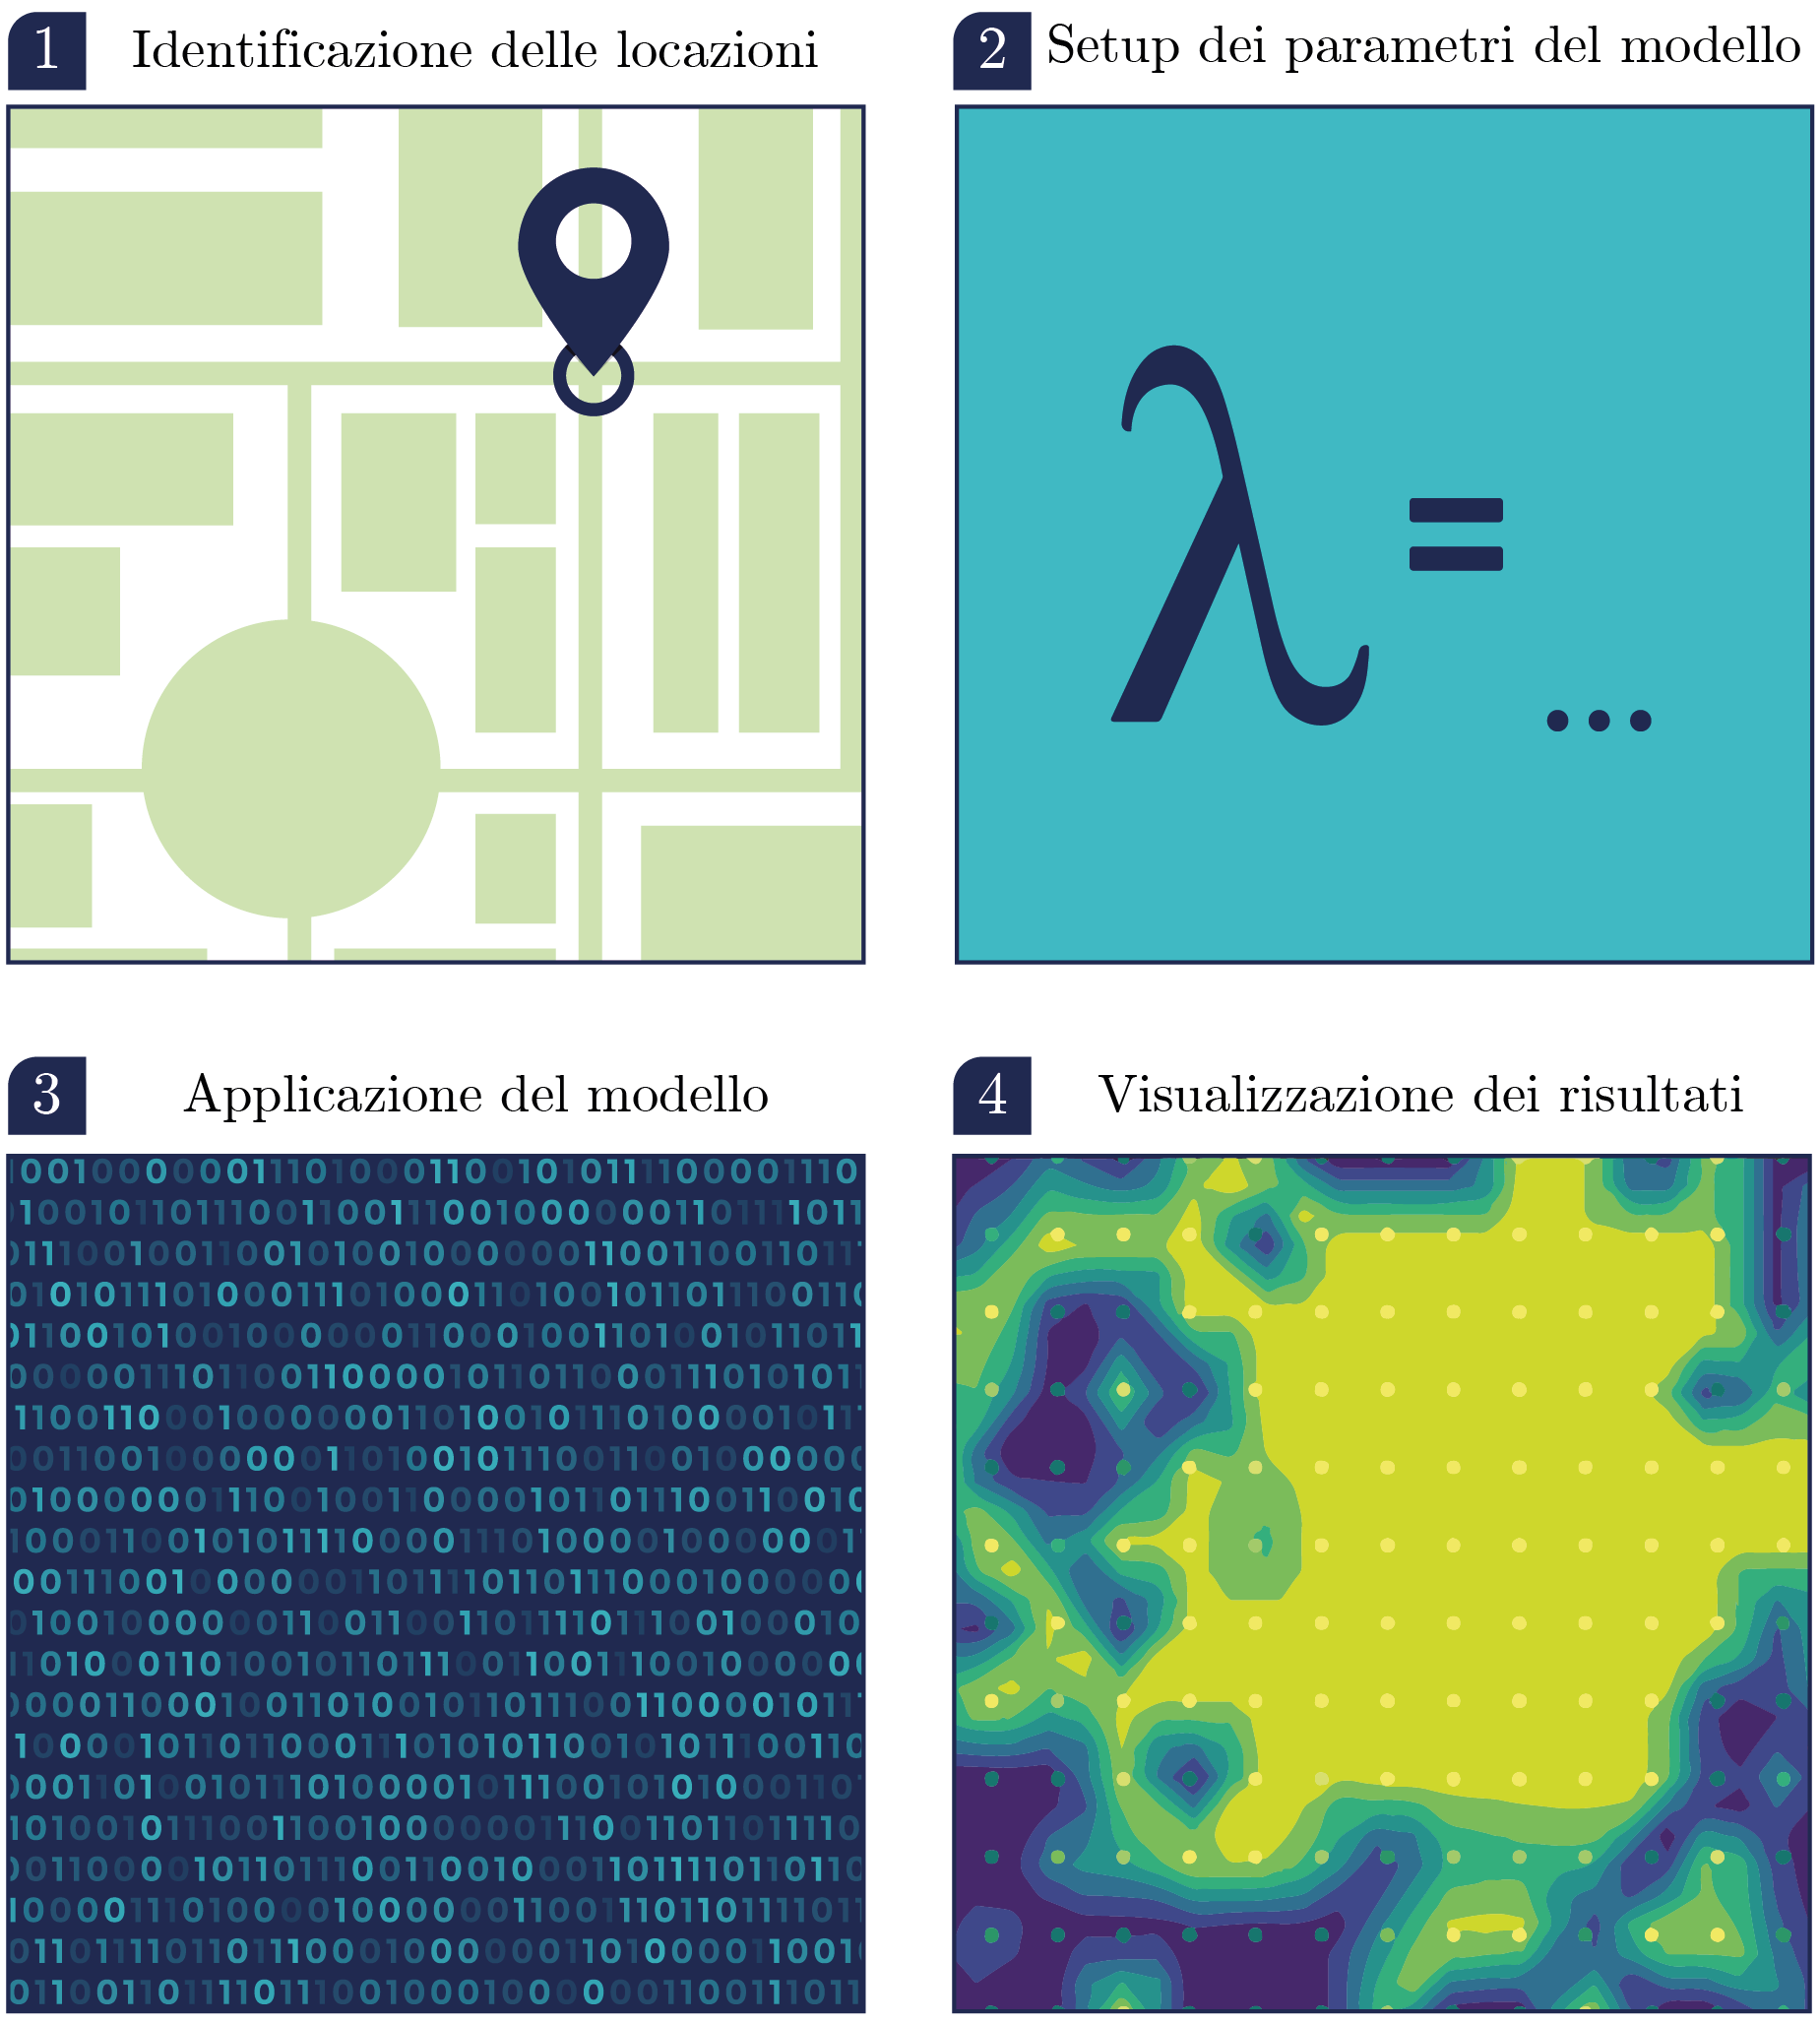
\includegraphics[width=\linewidth]{pipeline.png}
	\caption[Pipeline di sperimentazione]{L'immagine mostra la pipeline di sperimentazione utilizzata}
	\label{fig:pipeline}
\end{figure}


\section{Monitoraggio ambientale}
Lo scenario applicativo di monitoraggio ambientale si riferisce alla raccolta di dati utili al monitoraggio di parametri ambientali, come ad esempio: la temperatura, l'inquinamento acustico, la copertura e la qualità dei segnali wireless e molti altri. 

Per questa tipologia di MCS abbiamo preso in esame locazioni disposte a griglia ed equispaziate l'una dall'altra. Per fare ciò abbiamo opportunamente generato una griglia rettangolare più grande possibile che ricadesse all'interno dei confini geografici della macroarea di Pechino. L'idea è che i dati di tipo ambientale varino in modo molto meno netto rispetto a dati di altro tipo come possono essere quelli del traffico, per questa ragione la distanza tra le locazioni è nell'ordine dei chilometri, così da poter captare variazioni significative nei dati che devono essere raccolti. 

\subsection{Generazione della griglia}
Per la generazione della griglia ci siamo avvalsi di \textit{Shapely} \cite{shapely} e \textit{PiProj} \cite{pyproj}.
Dopo aver scelto gli estremi dell'area su cui generare la griglia, abbiamo impiegato queste librerie per ottenere le locazioni corrette. Grazie alla classe Point di Shapely e alle proiezioni fornite da PyProj, abbiamo iterativamente selezionato i punti della griglia prendendoli a distanza regolare sulla proiezione bidimensionale ottenuta. Successivamente li abbiamo riproiettati  a coordinate GCS sempre grazie a PyProj. 

Una volta ottenuta la griglia abbiamo provveduto a serializzarla per la successiva applicazione del modello.

Grazie a folium \cite{folium}, in Figura \ref{fig:grid}, possiamo visualizzare la griglia ottenuta.
Le locazioni sono identificate dai cerchi blu.
In sovraimpressione sono presenti alcune delle traiettorie di Augmented Geolife.

\begin{figure}[H]
	\centering 
	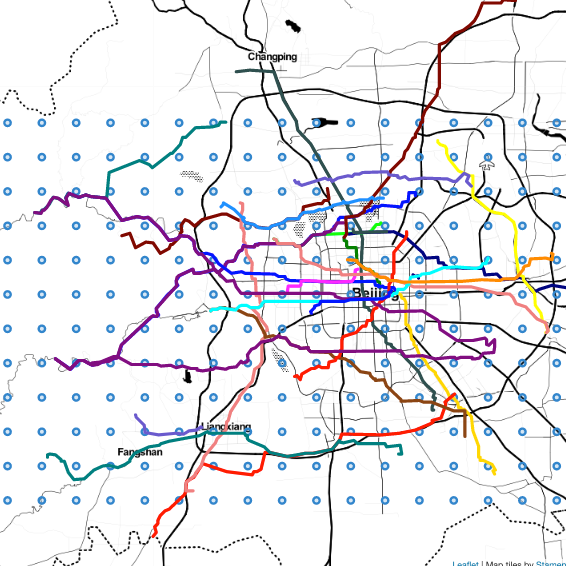
\includegraphics[width=\linewidth]{grid_folium.png}
	\caption[Griglia visualizzata con folium]{La griglia visualizzata per mezzo di folium}
	\label{fig:grid}
\end{figure}

\subsection{Risultati del modello di coverage}
Le Figure \ref{fig:grid_coverage1}, \ref{fig:grid_coverage2}, e \ref{fig:grid_coverage3}, mostrano i risultati ottenuti applicando il modello con differenti valori di lambda sulla griglia ottenuta. 
Dalle mappe di calore e meshgrid ottenute, si può notare come la Data Coverage vari al variare del paramentro $\lambda$, che modella la probabilità che gli utenti siano disposti ad accettare il detour verso le locazioni di raccolta dati.
Al crescere di $\lambda$ la Data Coverage migliora.
Le meshgrid e le mappe di calore sono state ottenute tramite interpolazione lineare sui risultati di Data Coverage ottenuti applicando il modello ad ogni singola locazione.

\begin{figure}[H]
	\centering
	\begin{subfigure}[b]{\linewidth}
		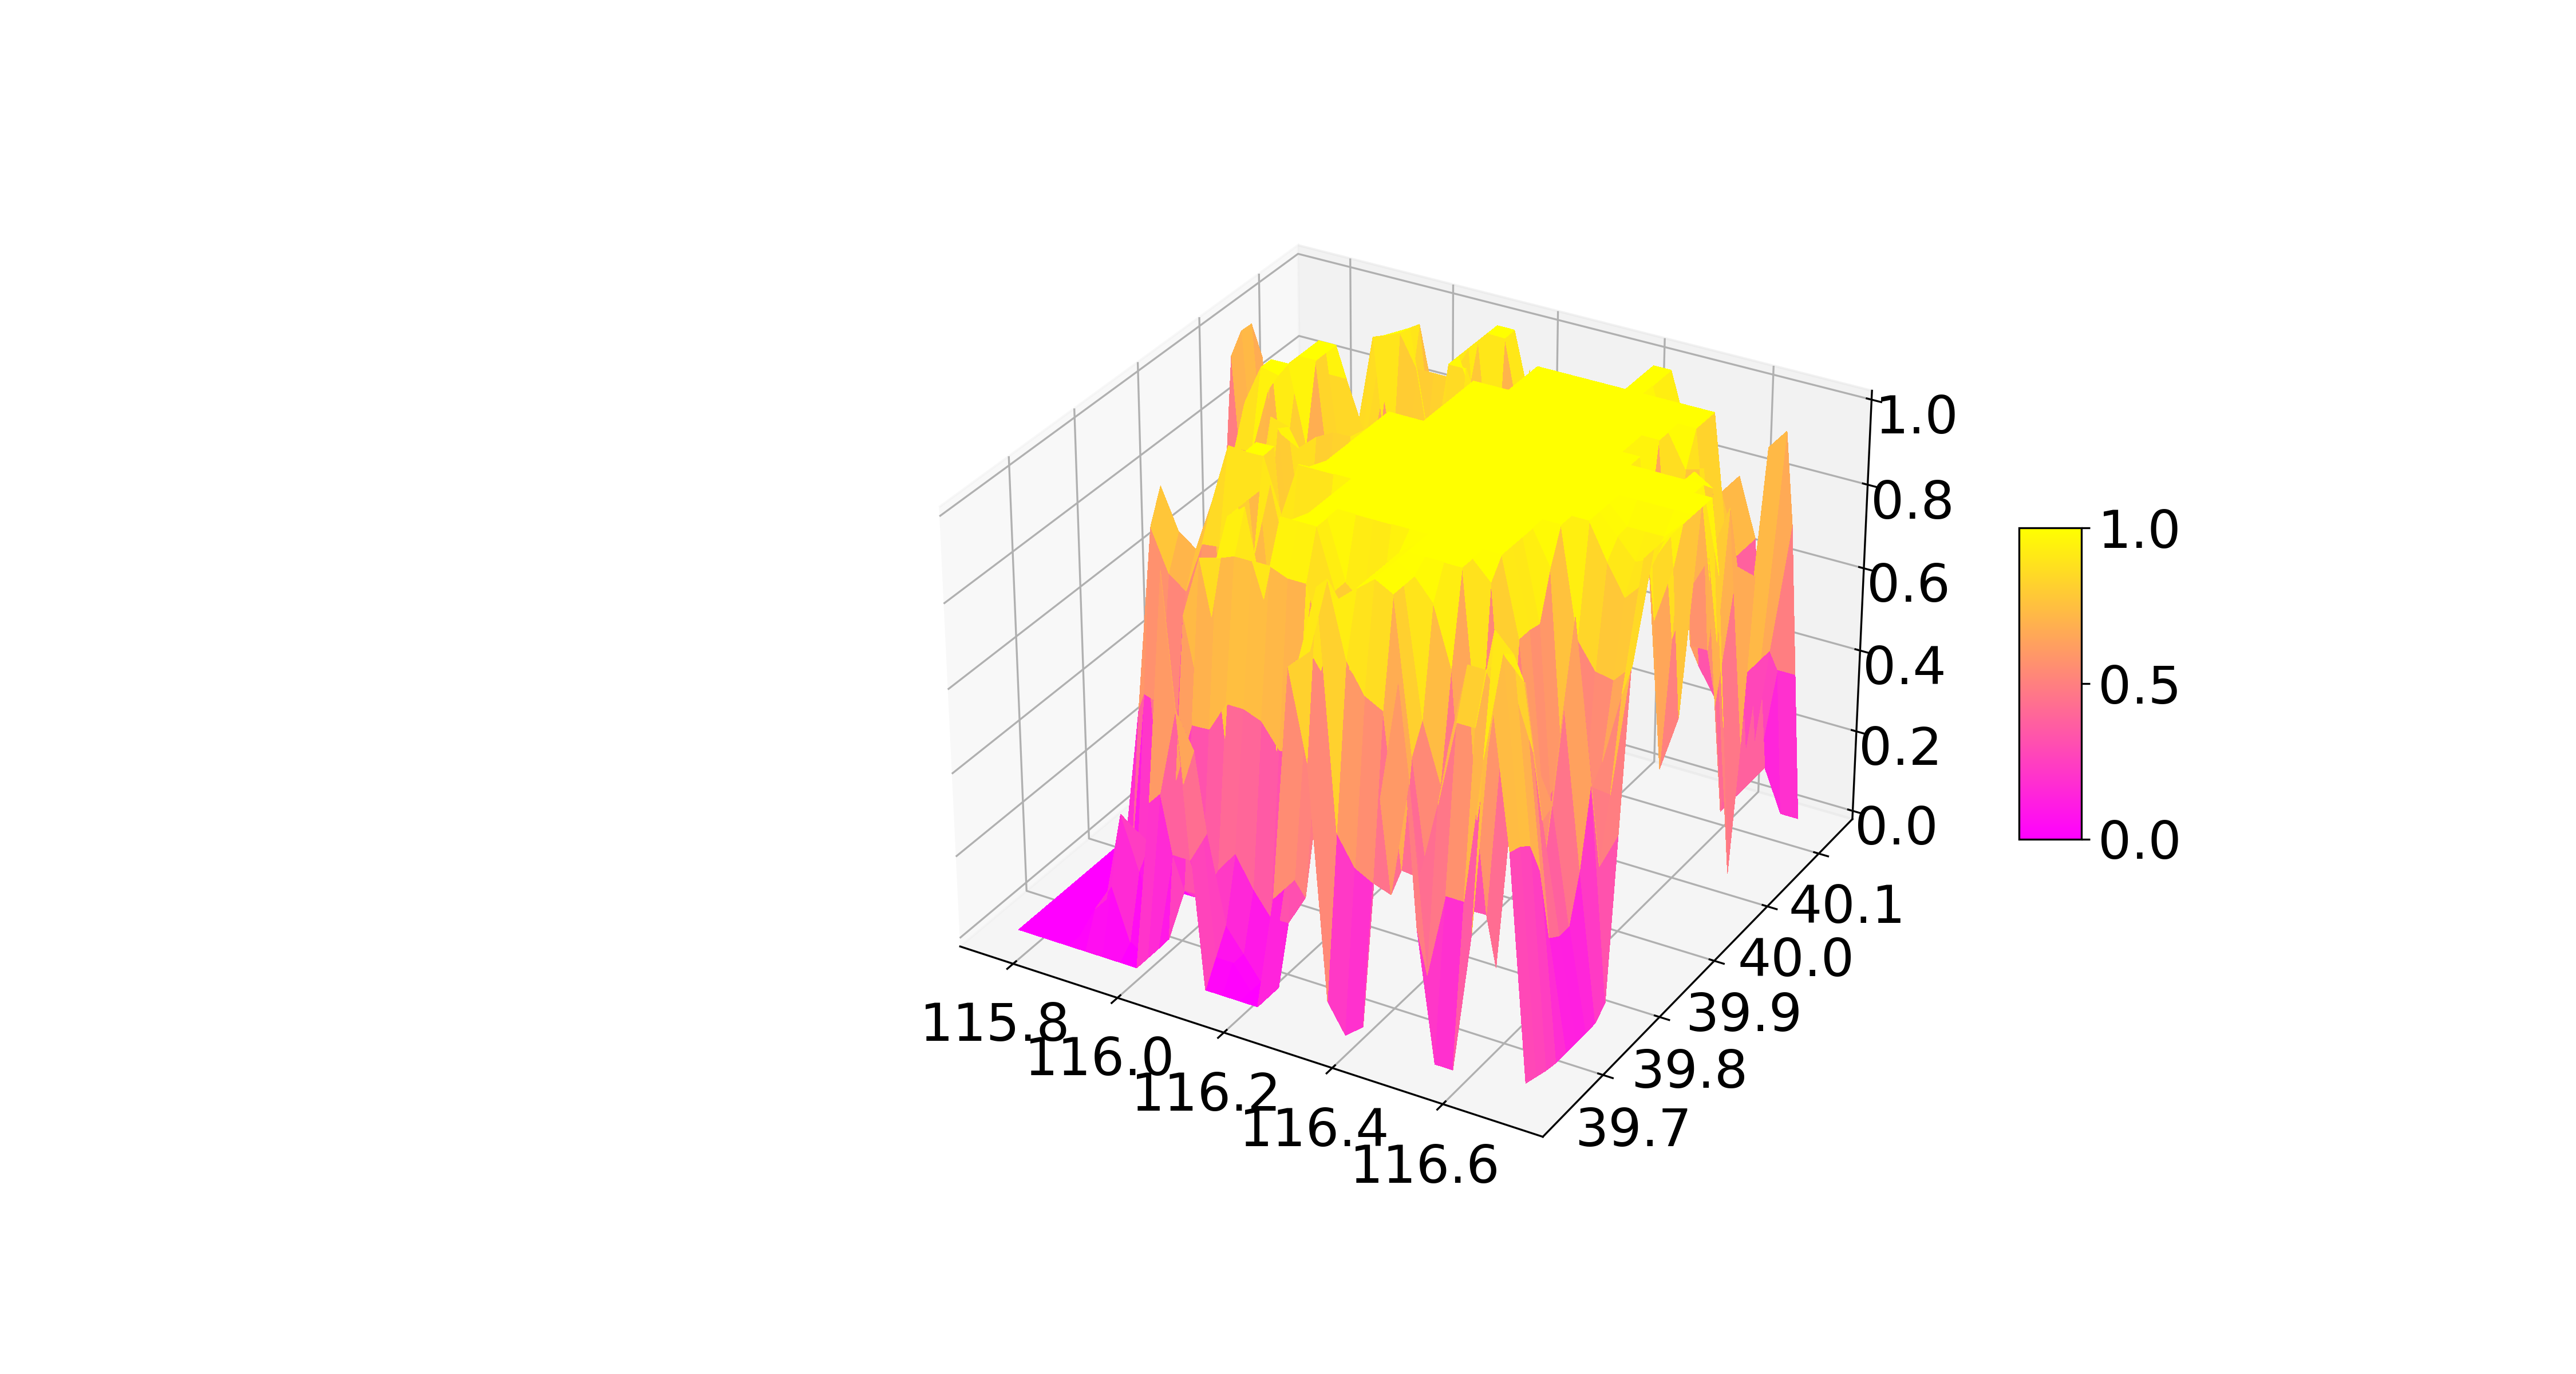
\includegraphics[width=\linewidth]{grid_coverages_0,01_lambda_3D_grid.png}
		\caption{Meshgrid ottenuta per $\lambda = 1/100$}
	\end{subfigure}
	\begin{subfigure}[b]{\linewidth}
		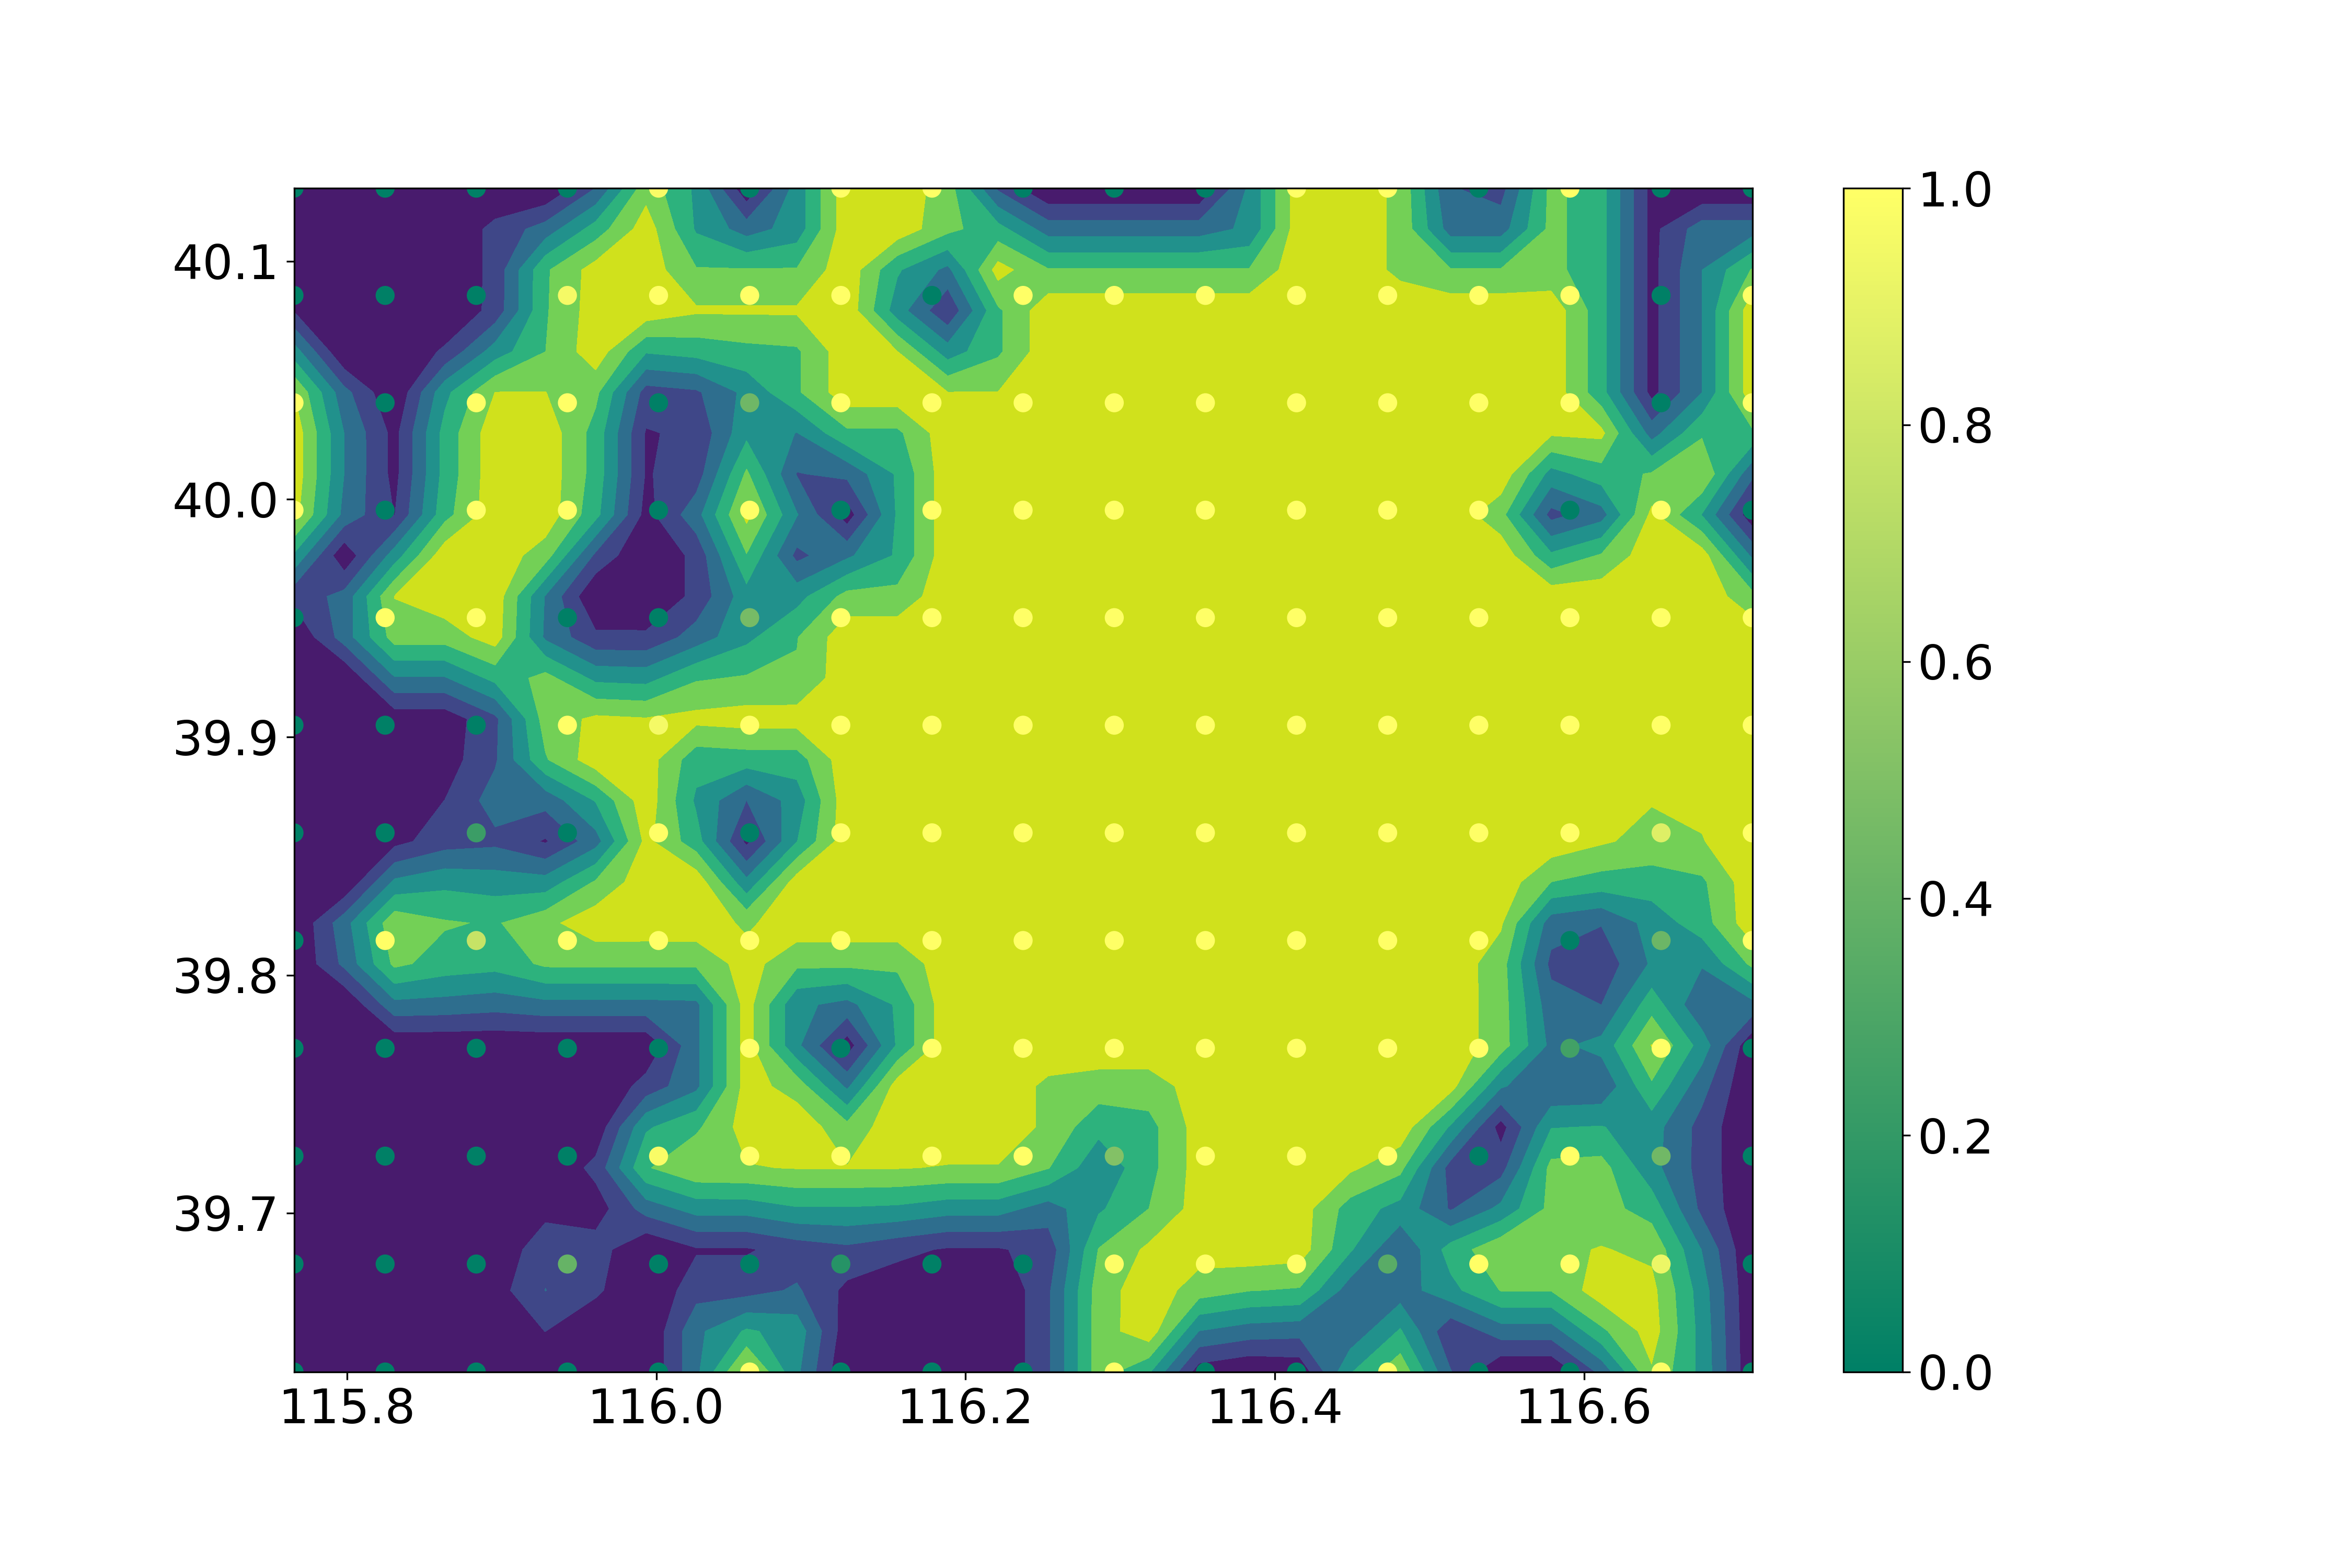
\includegraphics[width=\linewidth]{grid_coverages_0,01_lambda_heatmap.png}
		\caption{Mappa di calore ottenuta per $\lambda = 1/100$}
	\end{subfigure}
	\caption[Risultati griglia, $\lambda = 1/100$]{I risultati ottenuti applicando il modello alla griglia ambientale con $\lambda = 1/100$}
	\label{fig:grid_coverage1}
\end{figure}

\begin{figure}[H]
	\centering
	\begin{subfigure}[b]{\linewidth}
		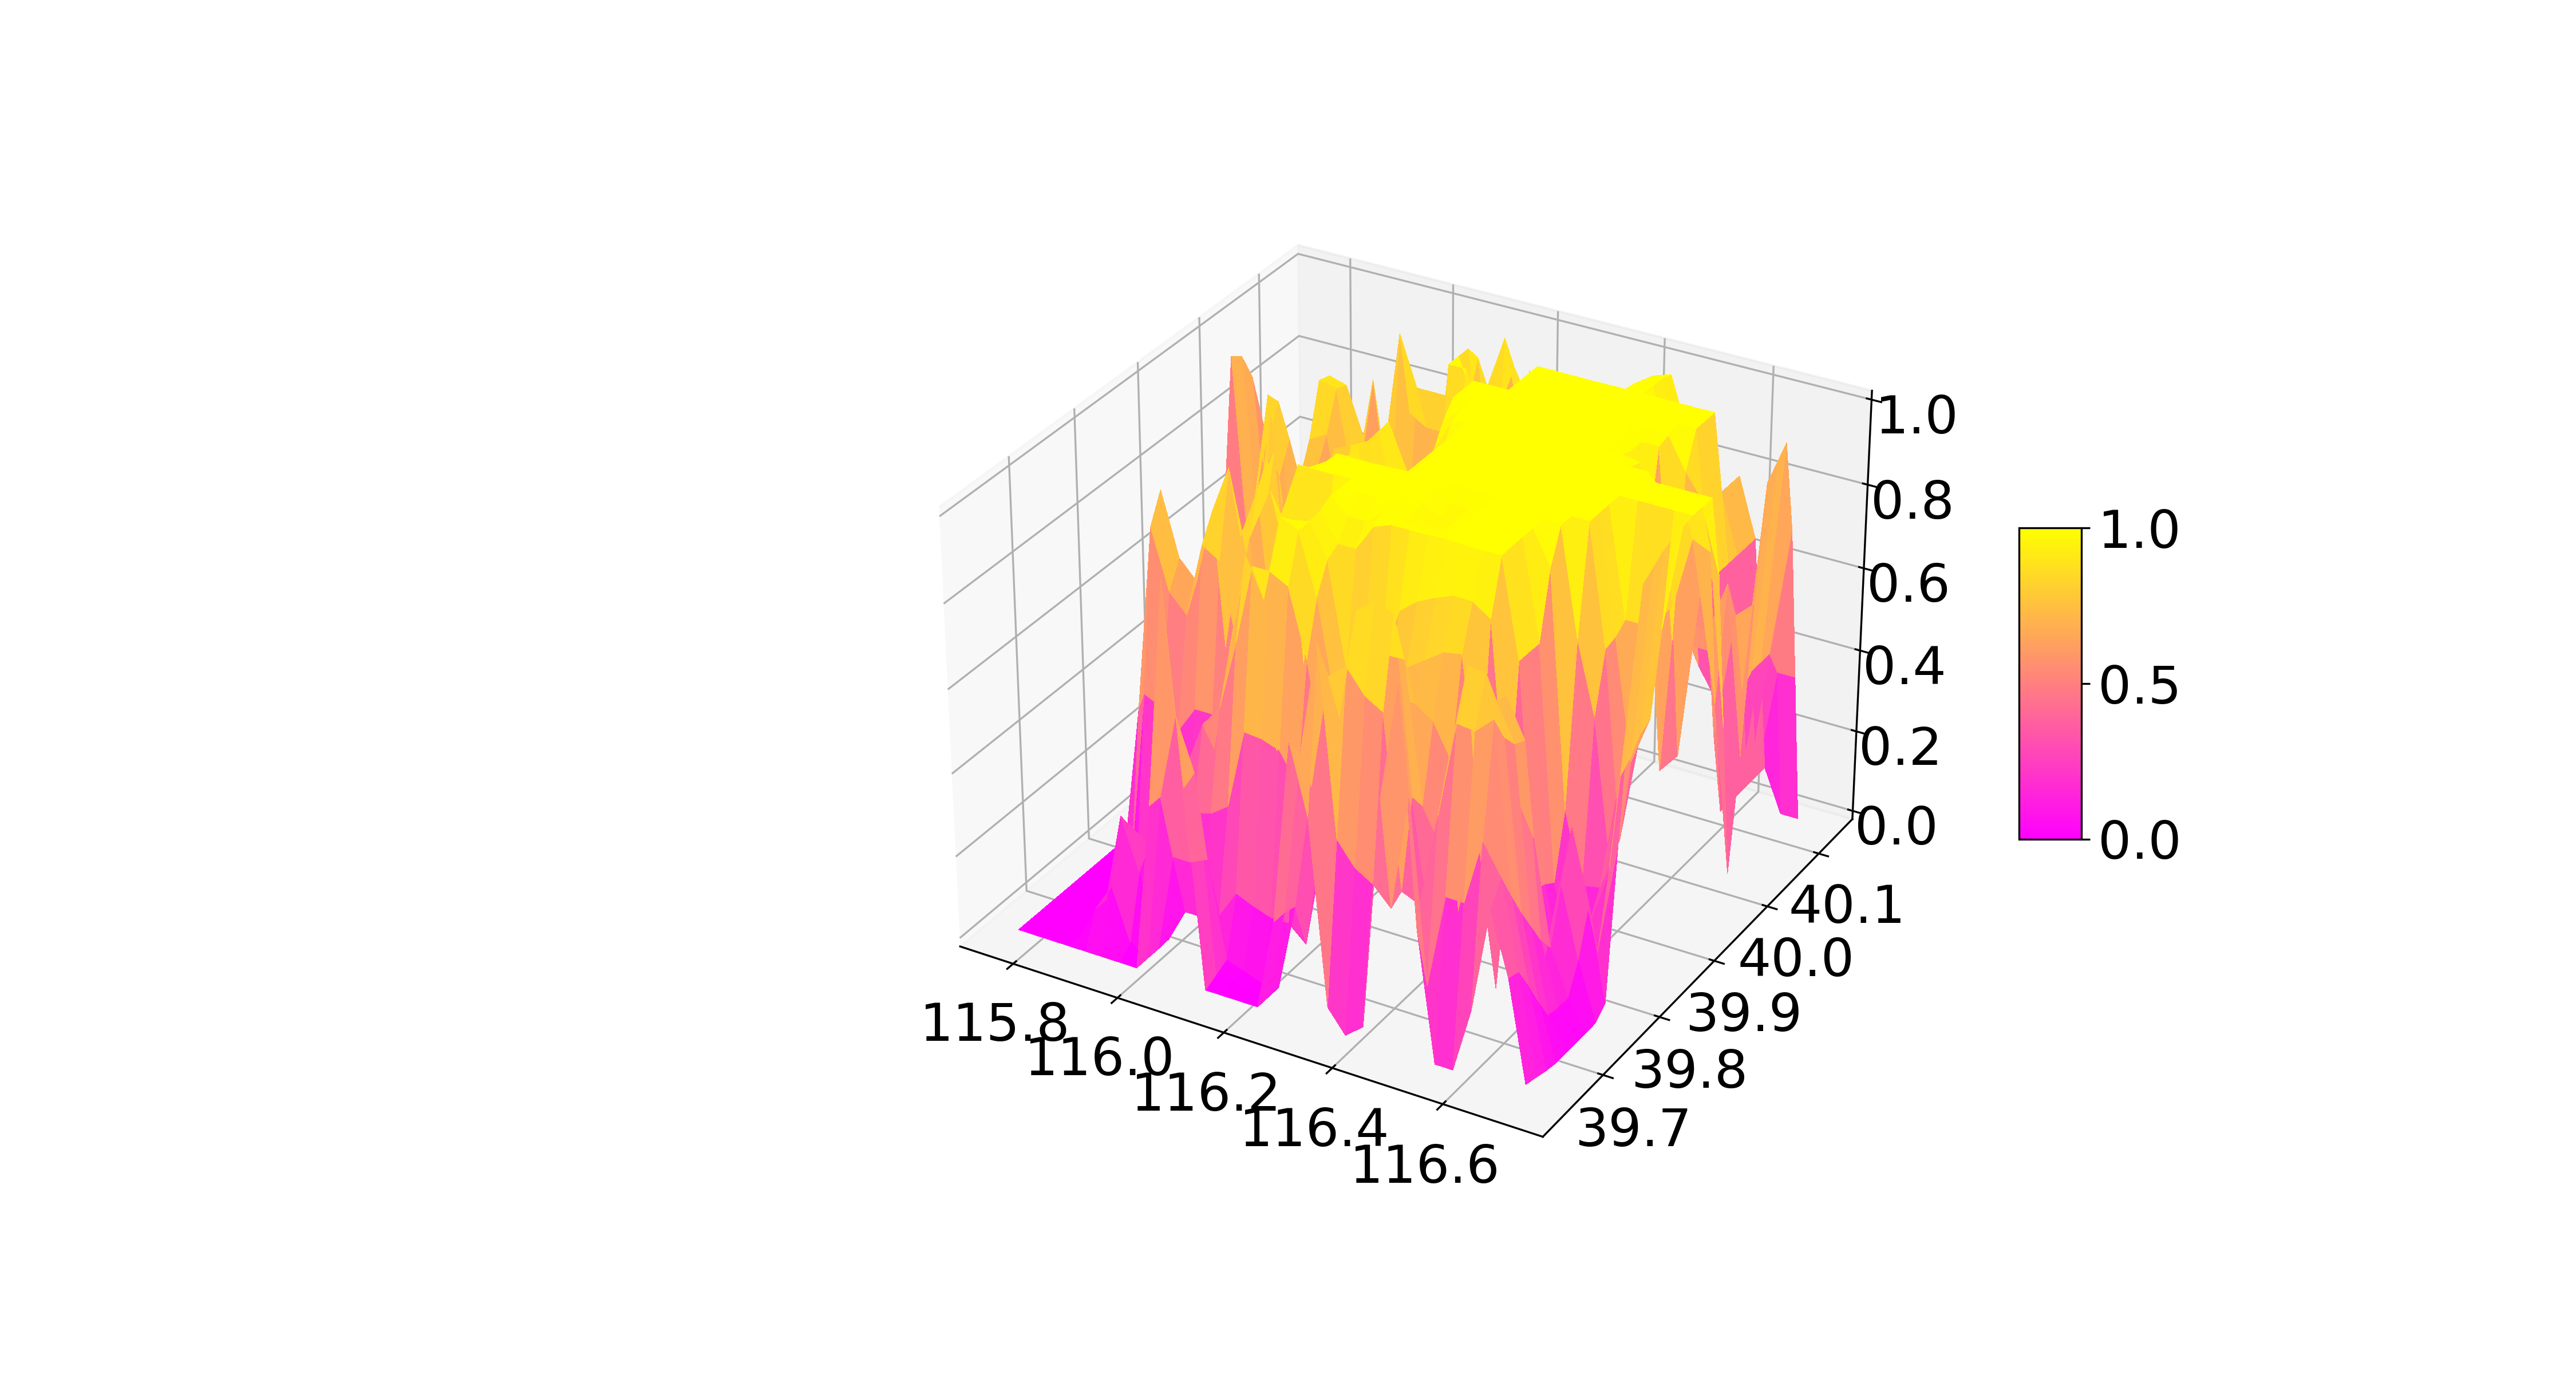
\includegraphics[width=\linewidth]{grid_coverages_0,00333333_lambda_3D_grid.png}
		\caption{Meshgrid ottenuta per $\lambda = 1/300$}
	\end{subfigure}
	\begin{subfigure}[b]{\linewidth}
		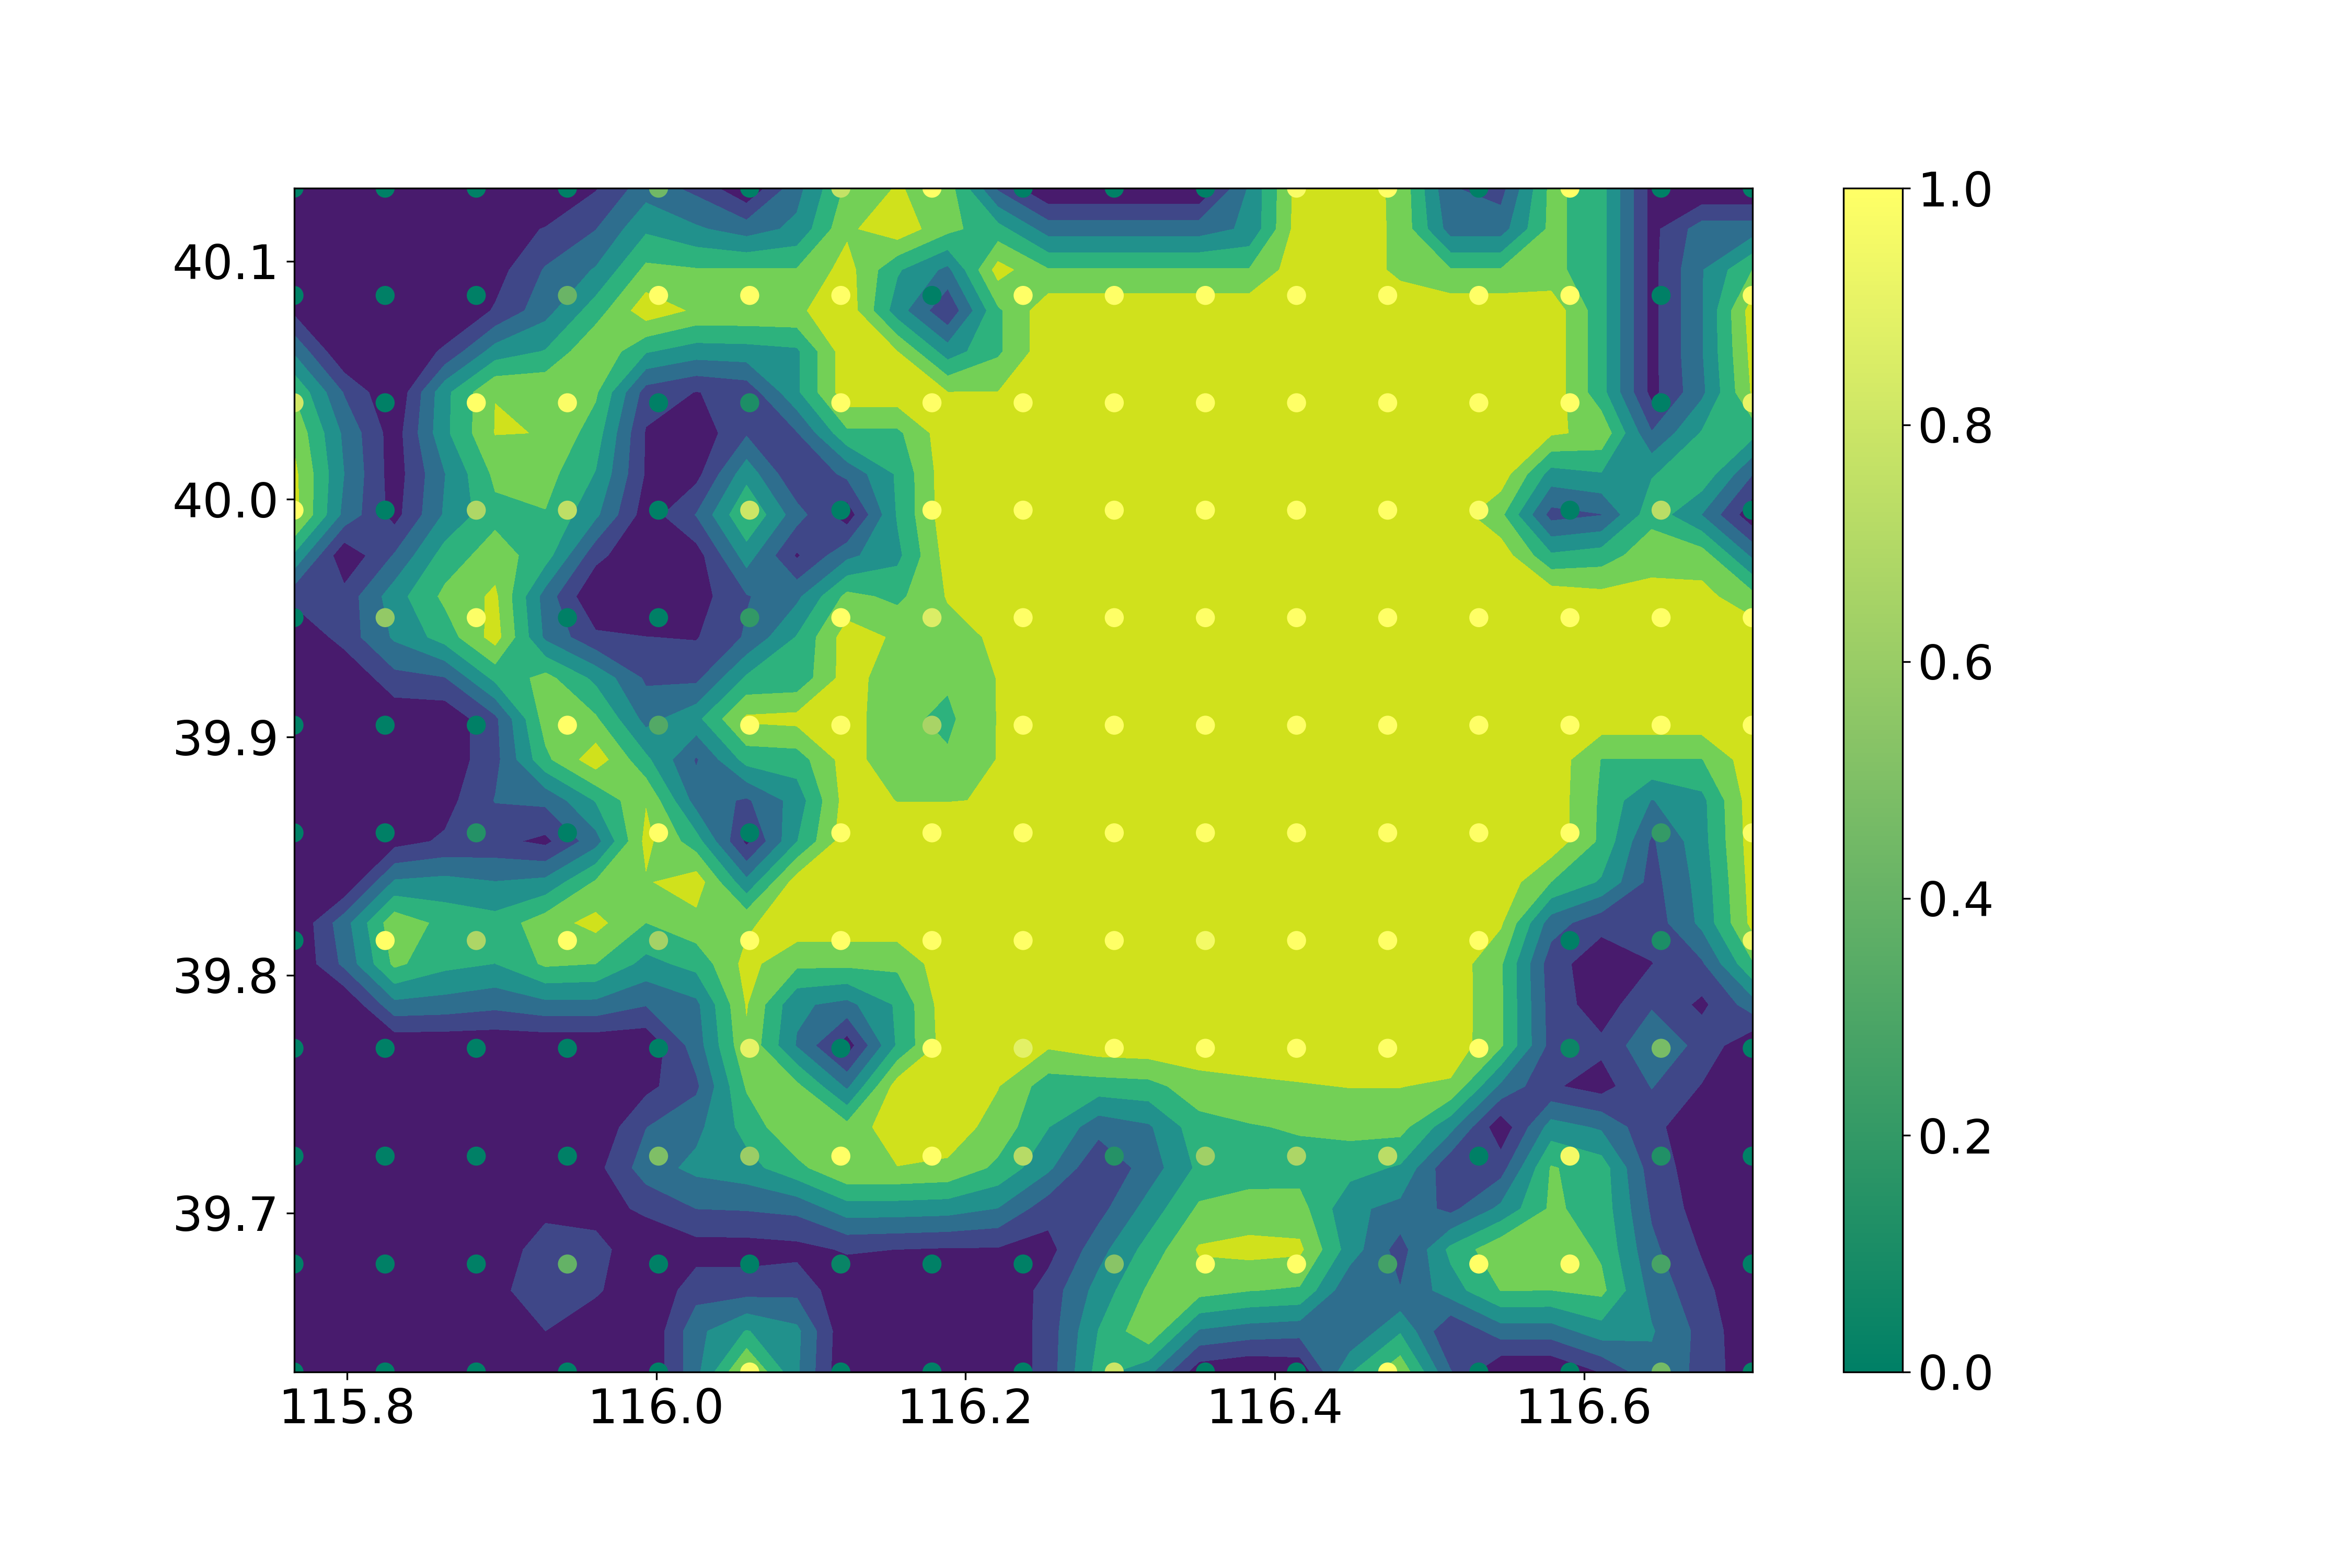
\includegraphics[width=\linewidth]{grid_coverages_0,00333333_lambda_heatmap.png}
		\caption{Mappa di calore ottenuta per $\lambda = 1/300$}
	\end{subfigure}
	\caption[Risultati griglia, $\lambda = 1/300$]{I risultati ottenuti applicando il modello alla griglia ambientale con $\lambda = 1/300$}
	\label{fig:grid_coverage2}
\end{figure}

\begin{figure}[H]
	\centering
	\begin{subfigure}[b]{\linewidth}
		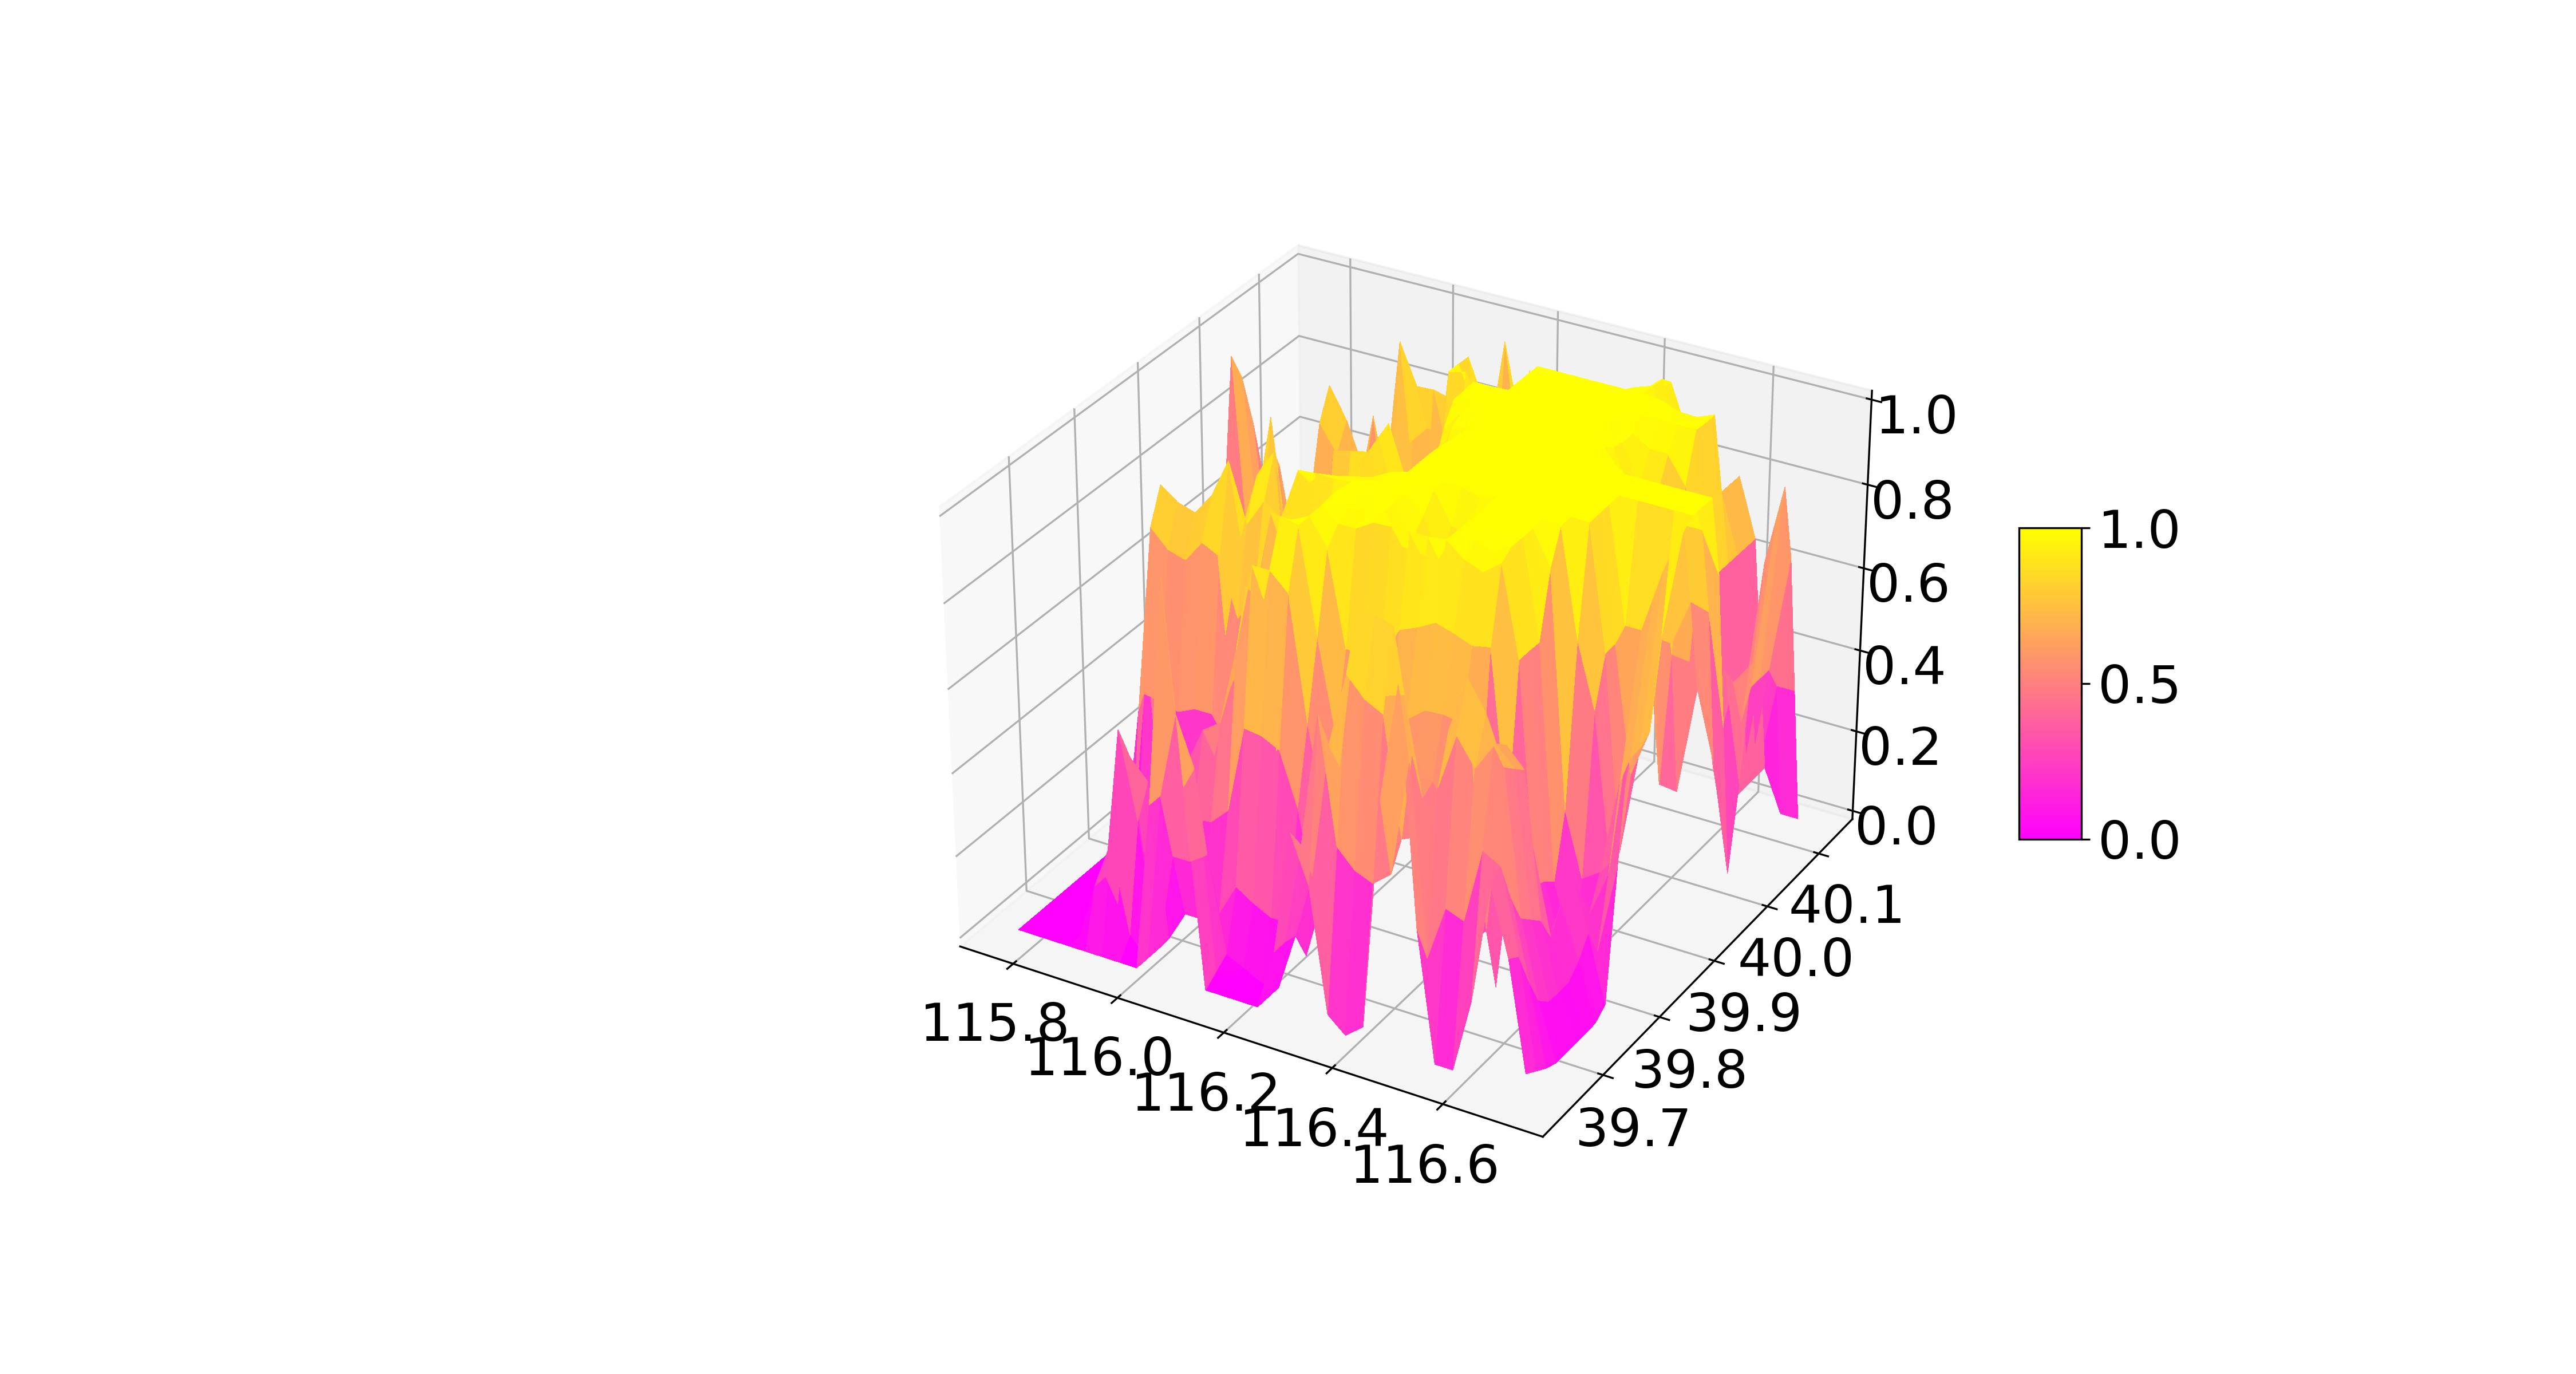
\includegraphics[width=\linewidth]{grid_coverages_0,00142857_lambda_3D_grid.png}
		\caption{Meshgrid ottenuta per $\lambda = 1/700$}
	\end{subfigure}
	\begin{subfigure}[b]{\linewidth}
		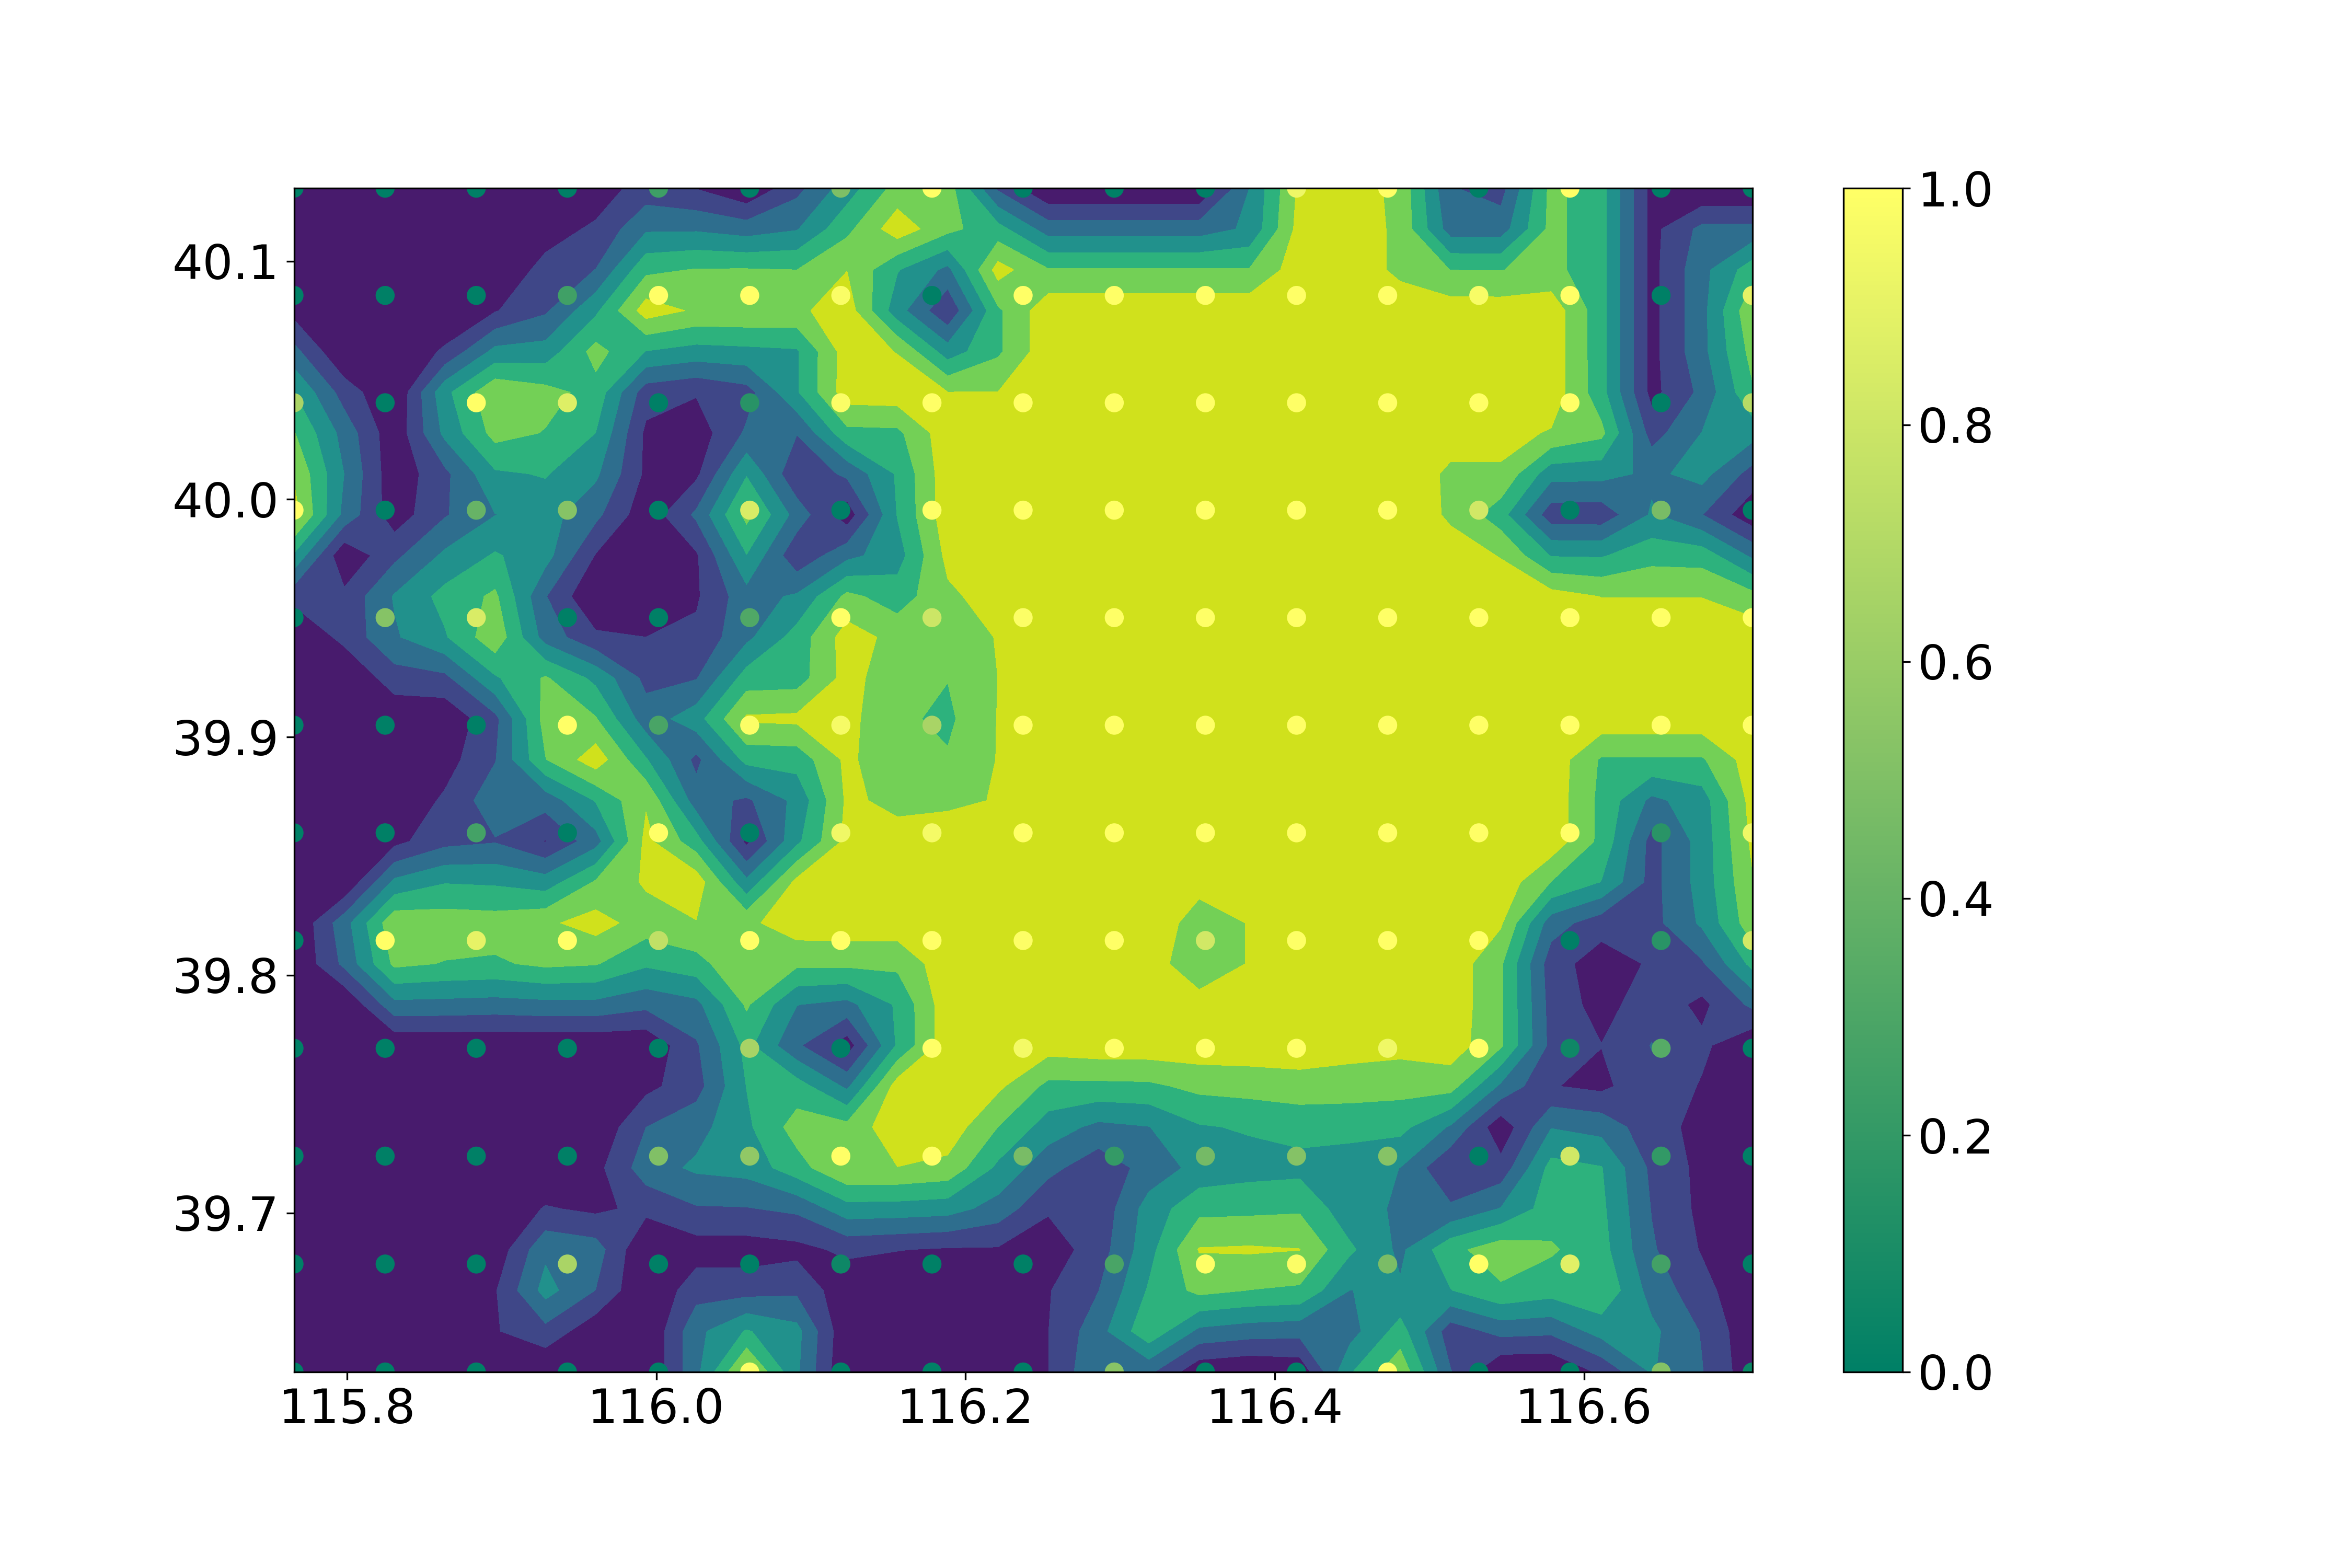
\includegraphics[width=\linewidth]{grid_coverages_0,00142857_lambda_heatmap.png}
		\caption{Mappa di calore ottenuta per $\lambda = 1/700$}
	\end{subfigure}
	\caption[Risultati griglia, $\lambda = 1/700$]{I risultati ottenuti applicando il modello alla griglia ambientale con $\lambda = 1/700$}
	\label{fig:grid_coverage3}
\end{figure}

\section{Flussi di traffico}
Con flusso di traffico si intende l'interazione tra viaggiatori, siano essi a piedi o su un qualsiasi altro mezzo di trasporto, e l'infrastruttura su cui essi si muovono.
I flussi di traffico vengono studiati per migliorare e rendere più efficienti le reti stradali, minimizzando congestioni e massimizzando il throughput della infrastruttura in termini di capacità effettiva di spostamento.

Riguardo al monitoraggio di tali flussi, ci siamo avvalsi di un data set con le coordinate geografiche di tutte le stazioni della metropolitana di Pechino estratto per mezzo di OSMnx \cite{osmnx}. Ipotizziamo che tali snodi principali siamo molto trafficati e siano visitati da una moltitudine di persone. Questo specifico scenario ci permette di valutare quale sia la portata del traffico umano attraverso questi luoghi. 

Il monitoraggio tramite MCS dei flussi di traffico, permette di raccogliere dati reali dalle infrastrutture di una Smart City permettendo a chi la gestisce di applicare nuove e migliori politiche urbanistiche e di gestione delle infrastrutture.

\subsection{OSMnx e metropolitane di Pechino}
Grazie alla funzione \textit{pois\_from\_point()} appartenente a OSMnx \cite{osmnx}, abbiamo estratto dal database di OpenStreetMap le coordinate GPS delle stazioni della metropolitana in un raggio di 50Km dal centro di Pechino.
Dopo aver ripulito il dataset estratto, abbiamo ottenuto un totale di 331 punti che abbiamo poi serializzato per il successivo calcolo della Data Coverage.

\subsection{Visualizzazione delle stazioni della metropolitana}
La Figura \ref{fig:subway} mostra le stazioni della metropolitana considerate, stampate grazie a folium \cite{folium}.
Analogamente alla griglia, la mappa ha in sovraimpressione alcune delle traiettorie del dataset. I cerchi blu rappresentano le singole stazioni della metropolitana.

\begin{figure}[H]
	\centering 
	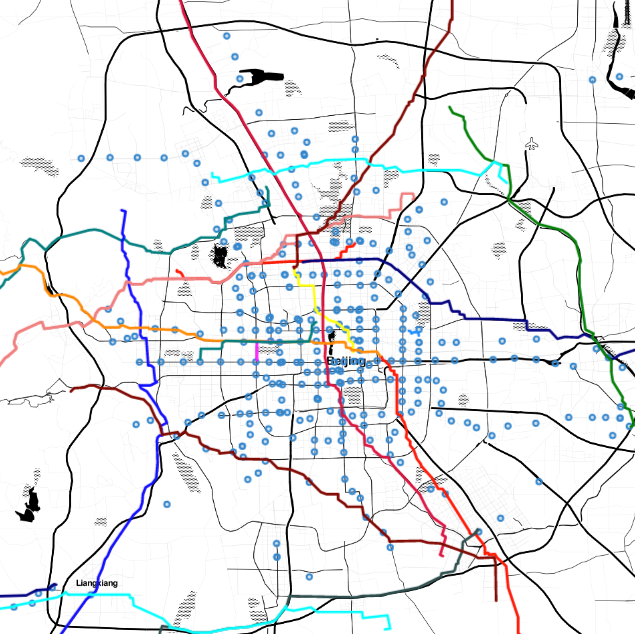
\includegraphics[width=\linewidth]{subway_folium.png}
	\caption[Mappa delle stazioni della metropolitana]{Le stazioni della metropolitana stampate grazie a folium}
	\label{fig:subway}
\end{figure}

\subsection{Risultati del modello di coverage}
Le Figure \ref{fig:subway_coverage1}, \ref{fig:subway_coverage2}, e \ref{fig:subway_coverage3}, mostrano i risultati ottenuti applicando il modello con differenti valori di lambda sulle uscite della metropolitana estratte per mezzo di OSMnx \cite{osmnx}. 

\begin{figure}[H]
	\centering
	\begin{subfigure}[b]{\linewidth}
		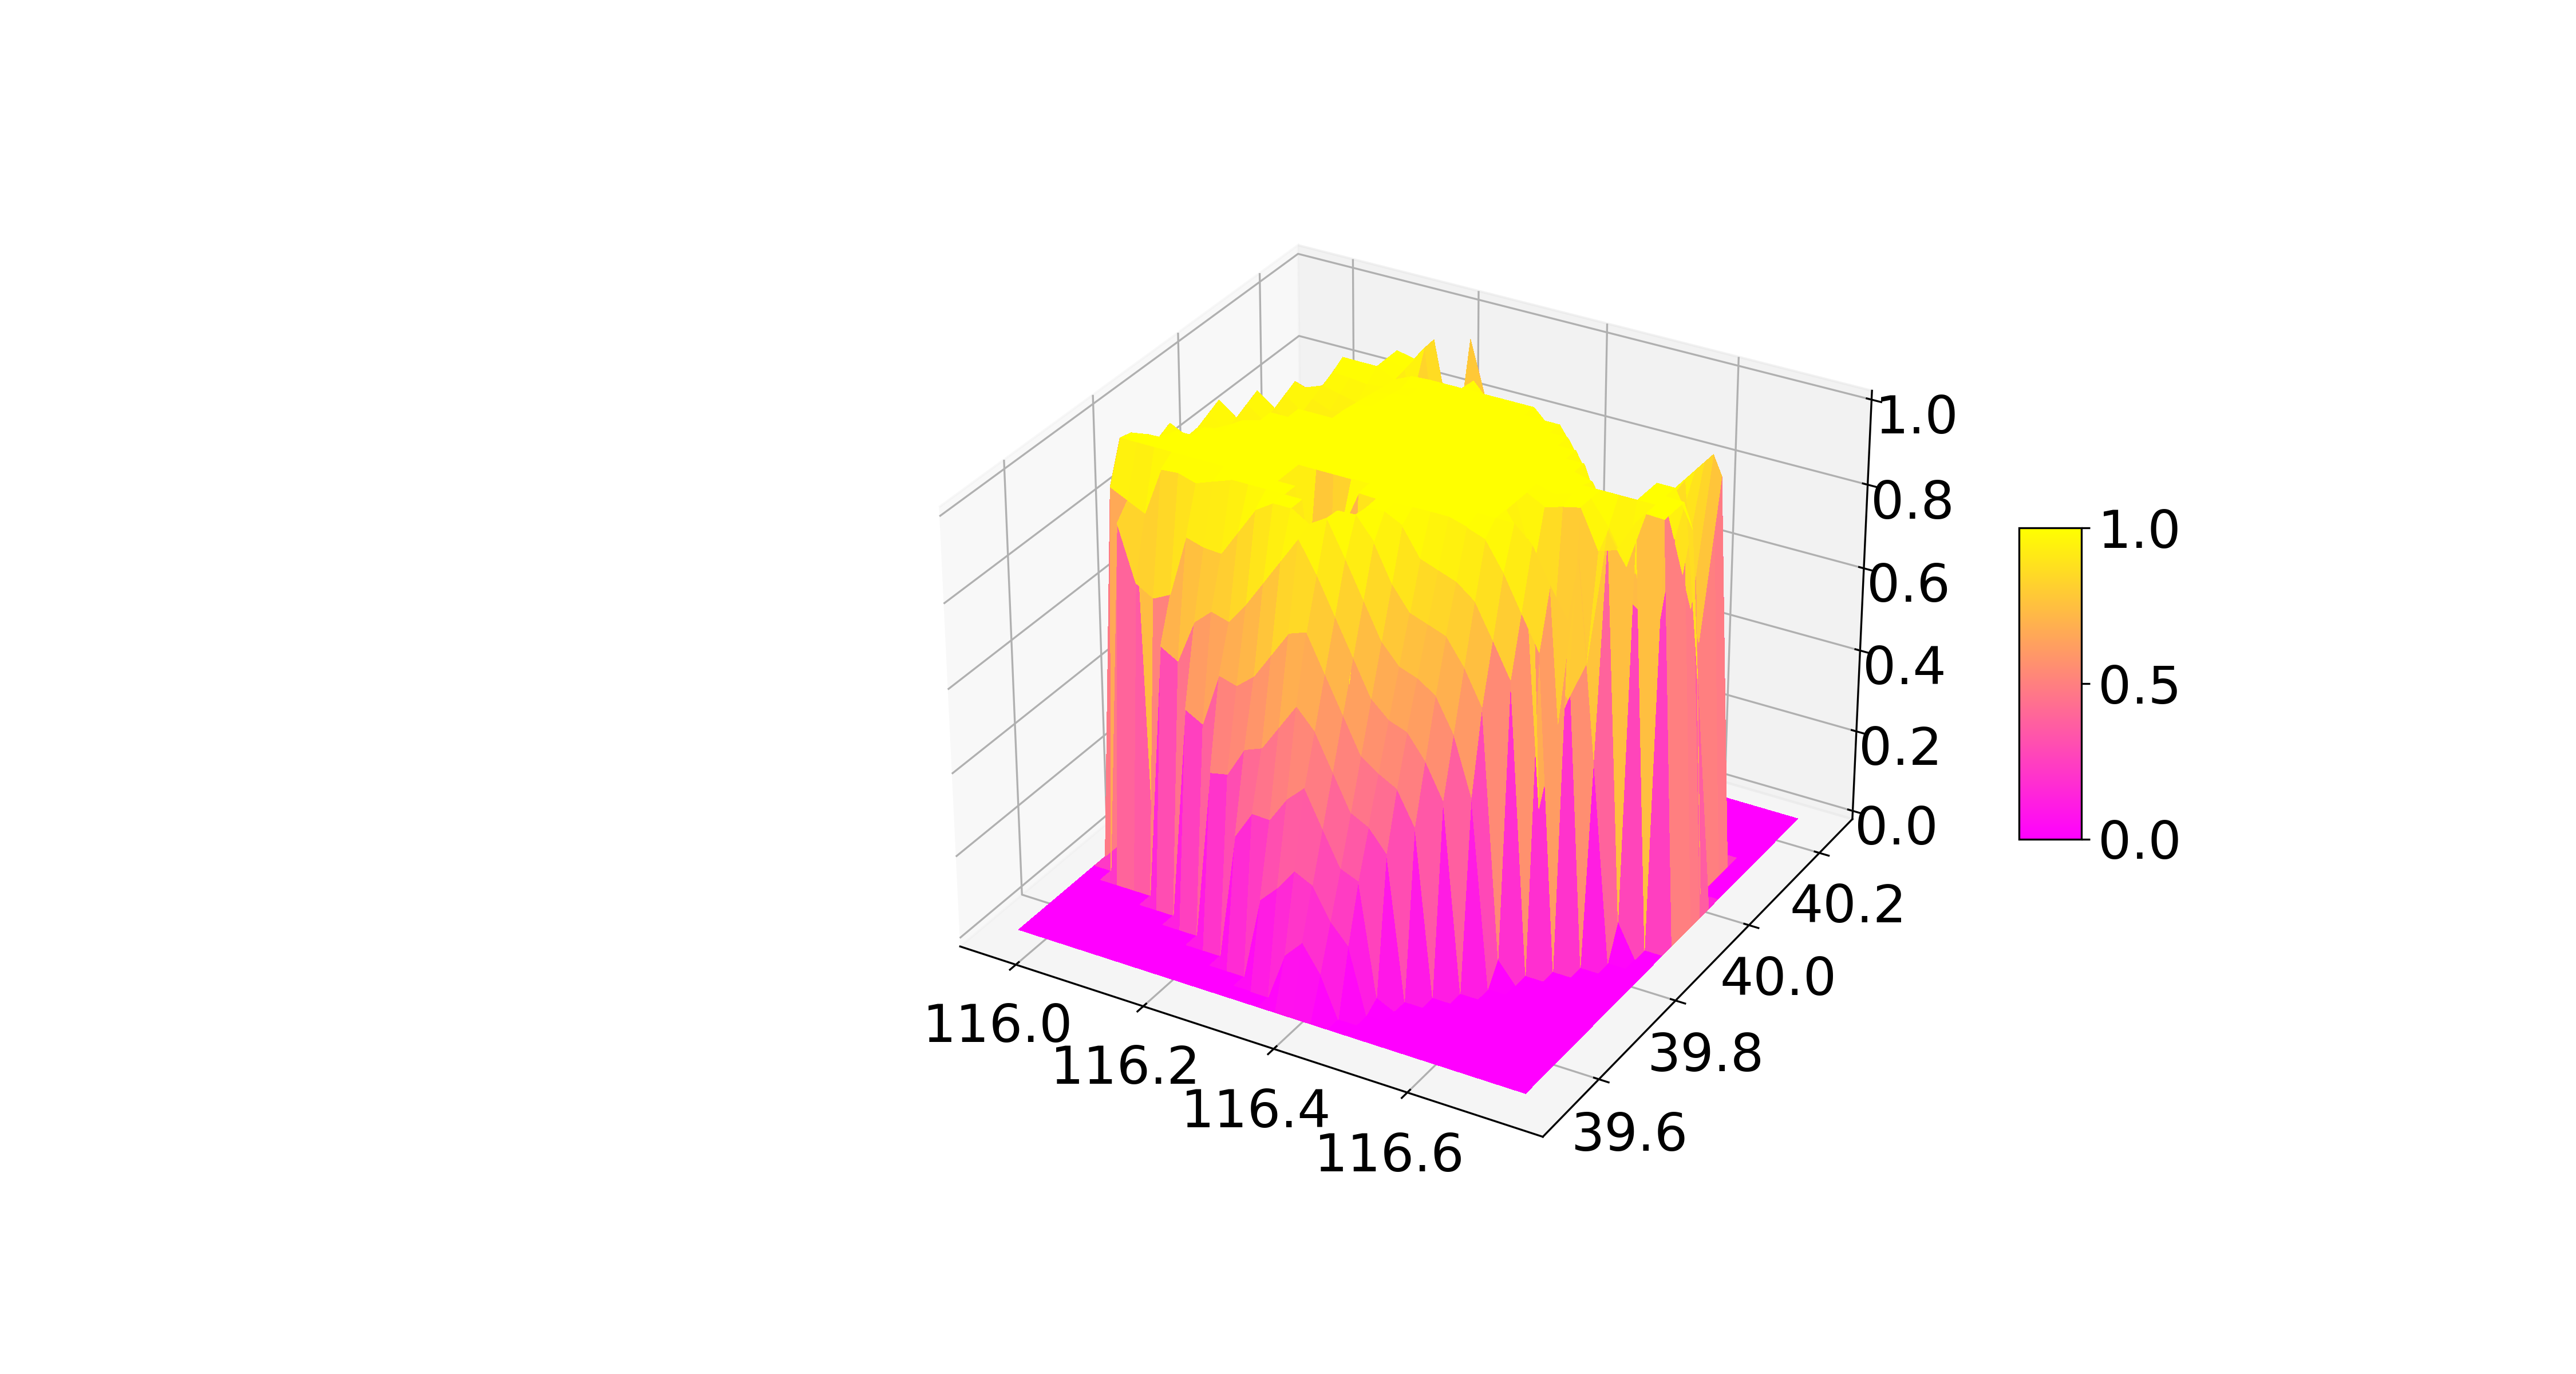
\includegraphics[width=\linewidth]{subway_coverages_0,01_lambda_3D_grid.png}
		\caption{Meshgrid ottenuta per $\lambda = 1/100$}
	\end{subfigure}
	\begin{subfigure}[b]{\linewidth}
		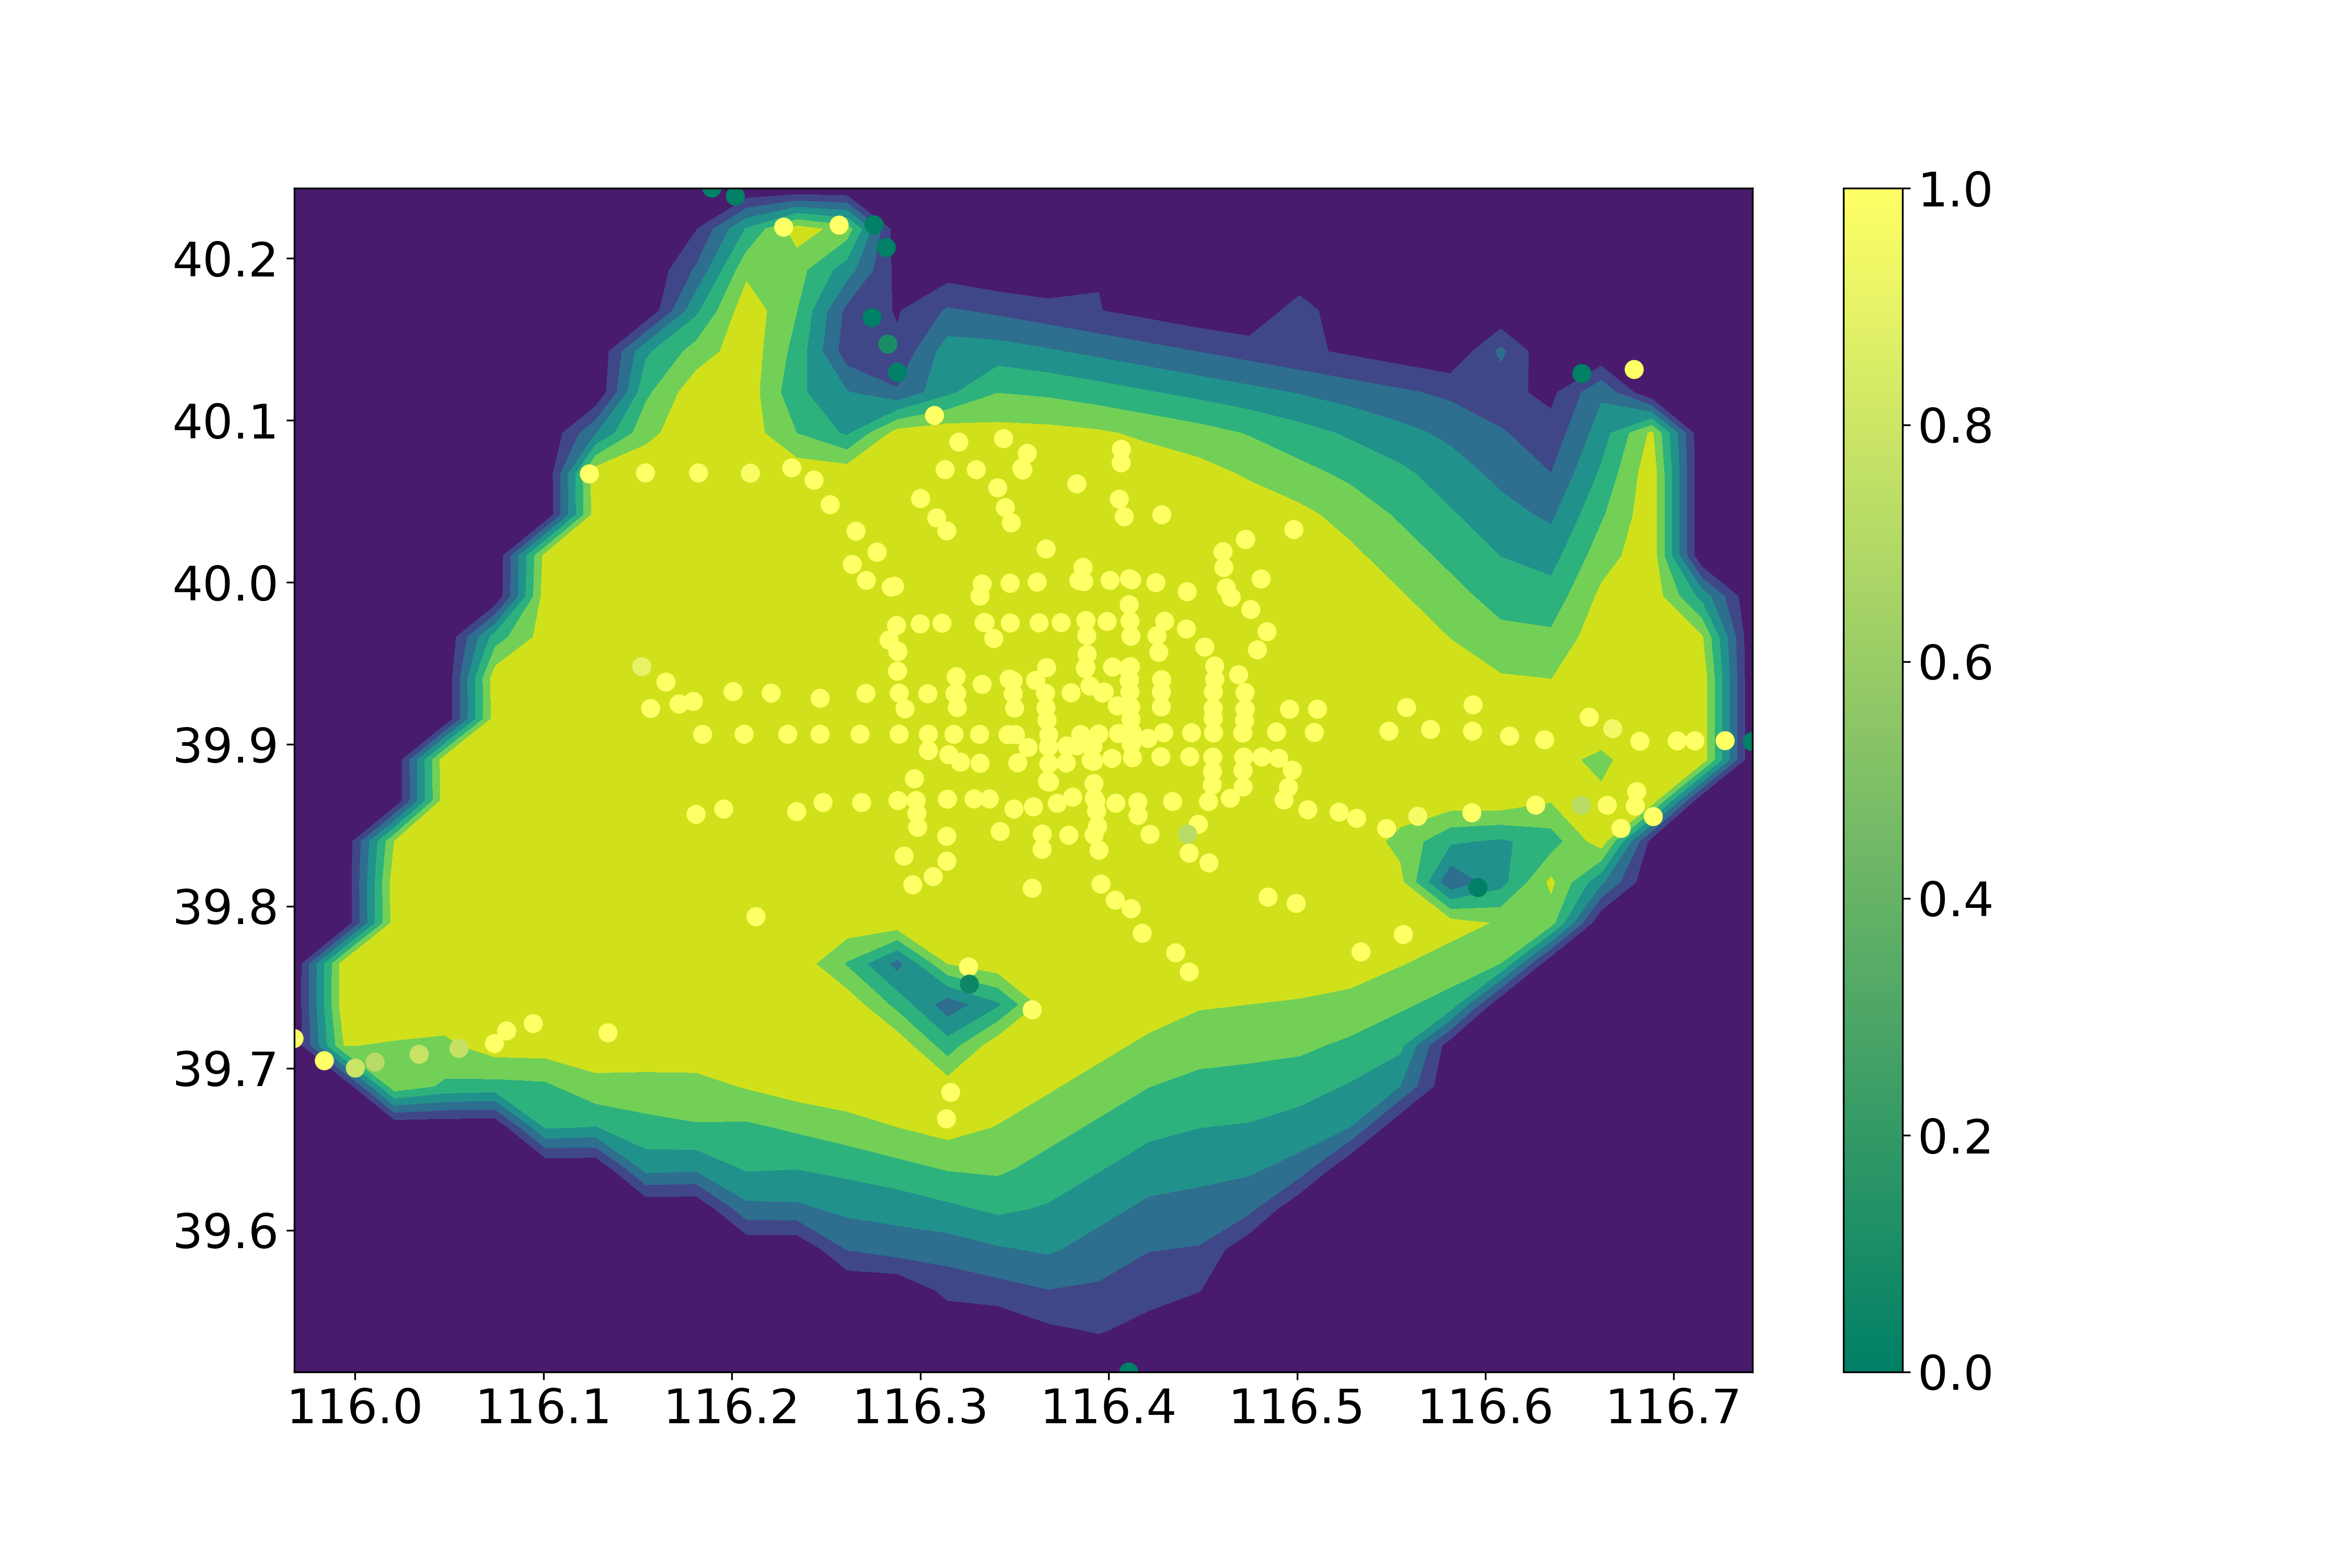
\includegraphics[width=\linewidth]{subway_coverages_0,01_lambda_heatmap.png}
		\caption{Mappa di calore ottenuta per $\lambda = 1/100$}
	\end{subfigure}
	\caption[Risultati metropolitana, $\lambda = 1/100$]{I risultati ottenuti applicando il modello alle uscite della metropolitana con $\lambda = 1/100$}
	\label{fig:subway_coverage1}
\end{figure}

\begin{figure}[H]
	\centering
	\begin{subfigure}[b]{\linewidth}
		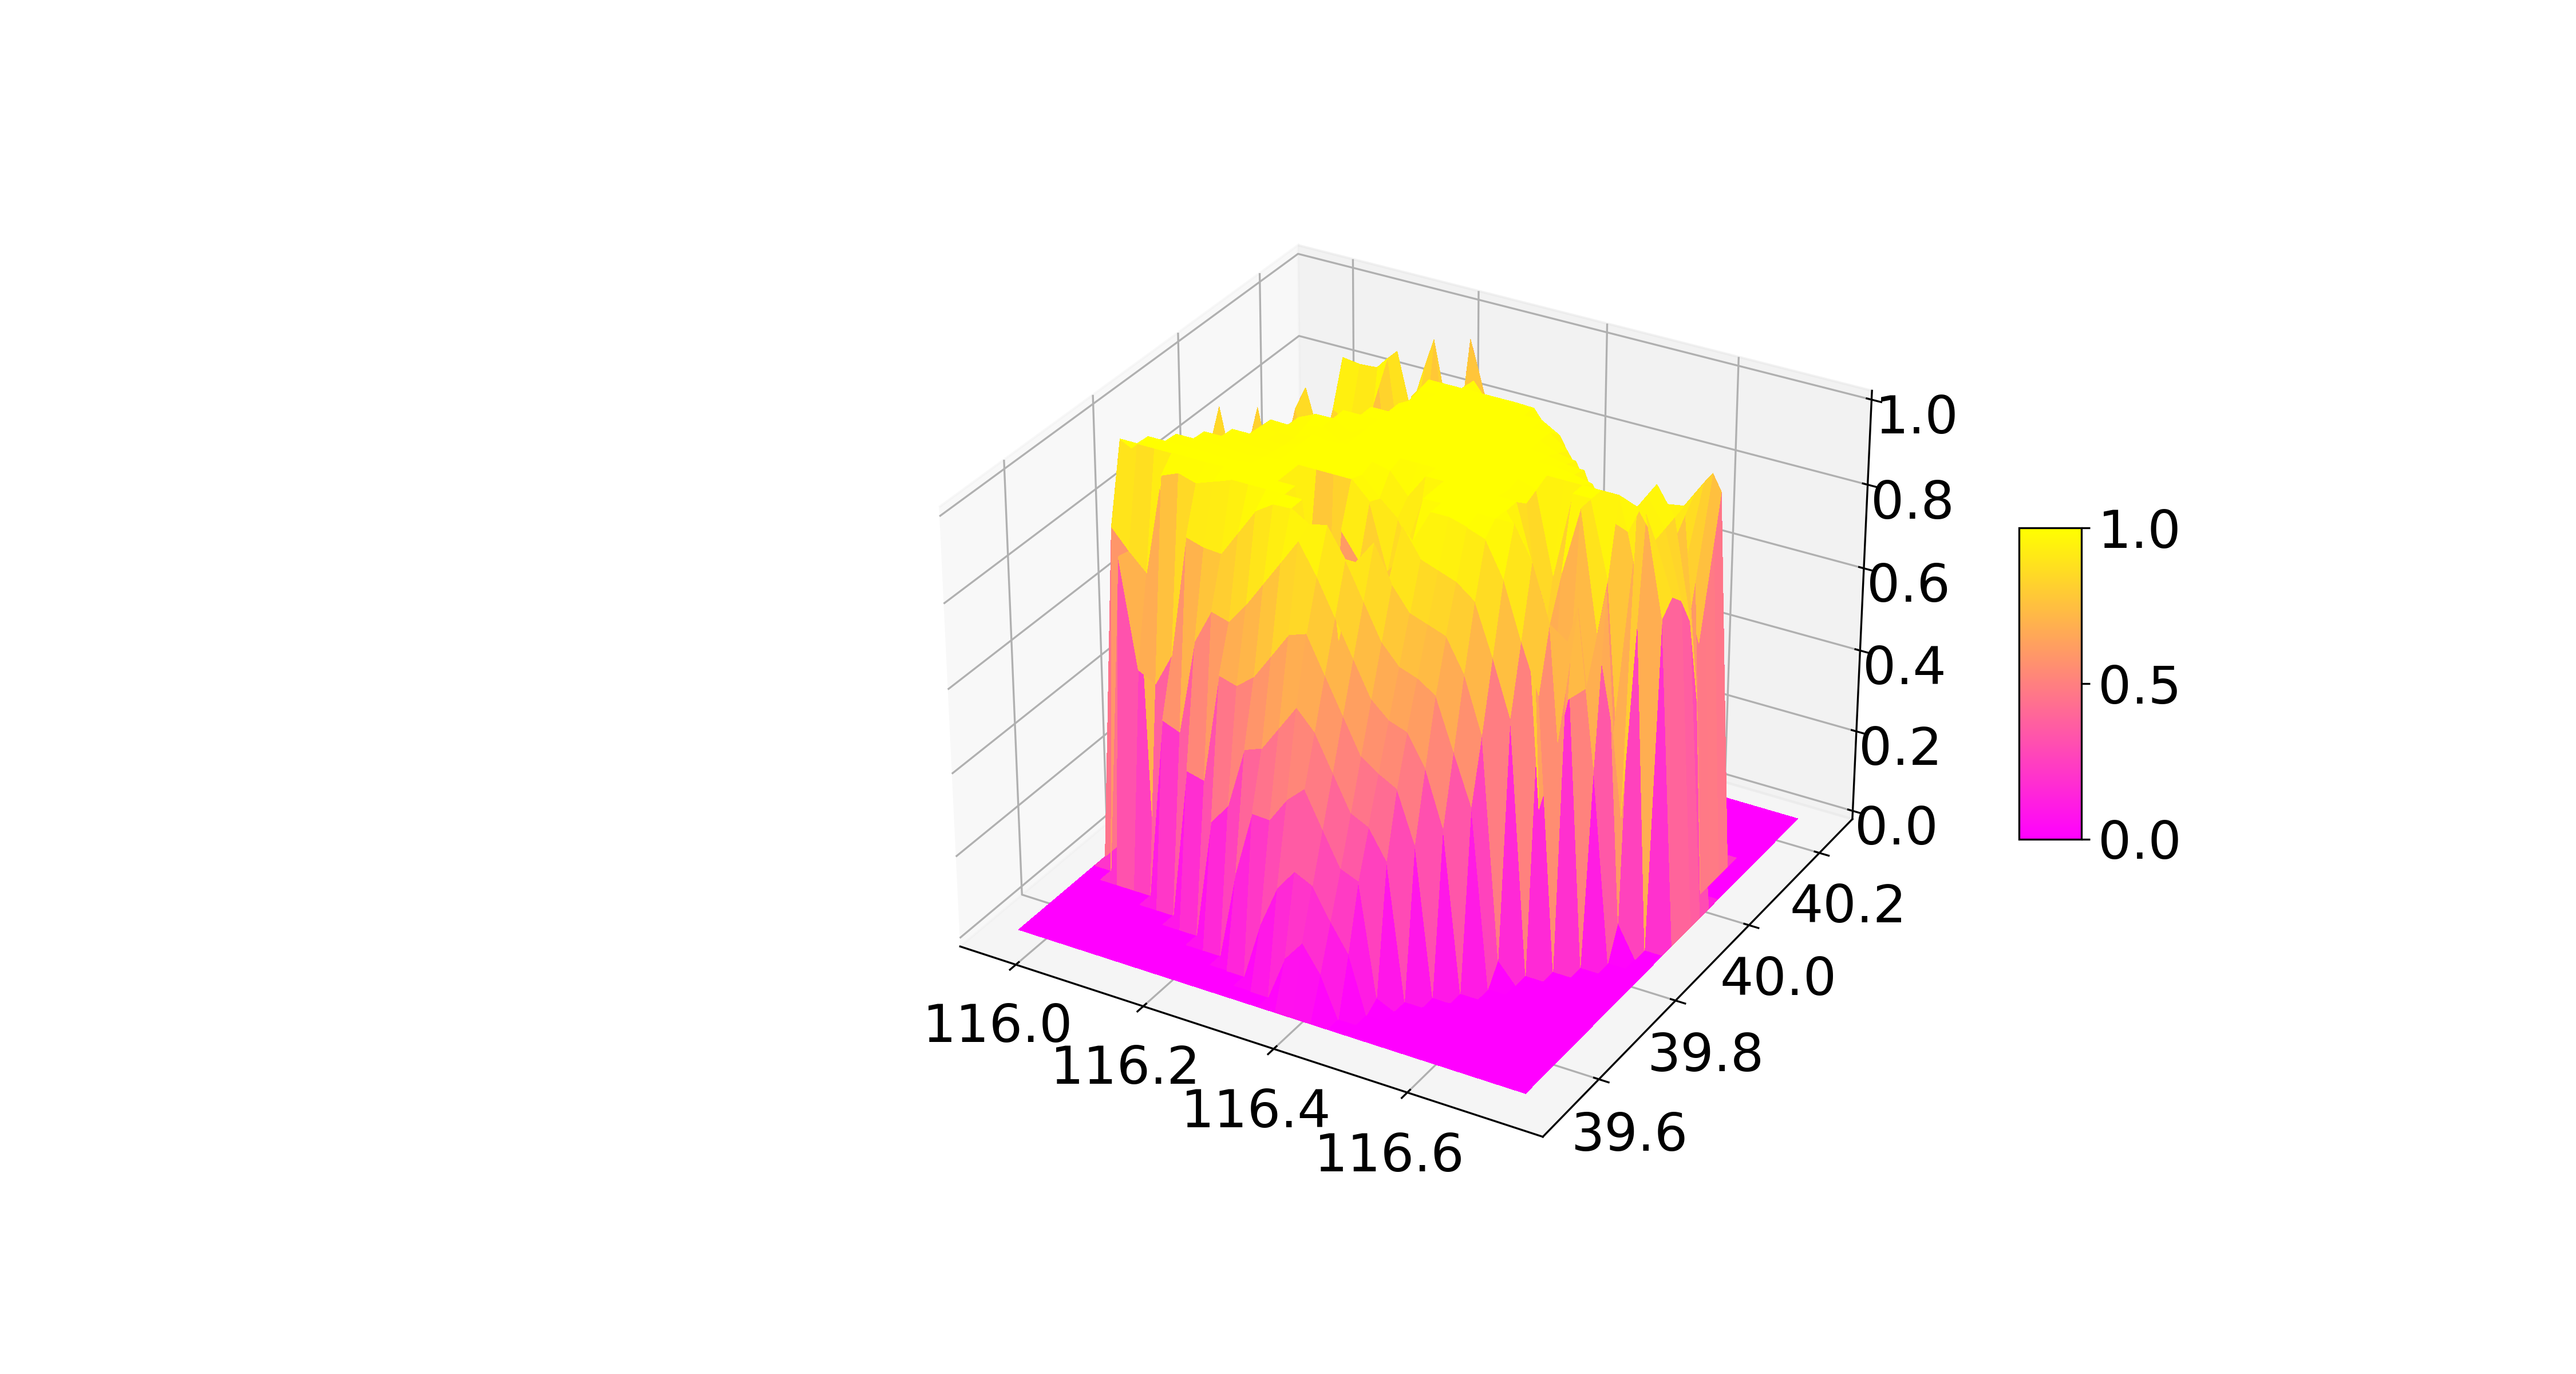
\includegraphics[width=\linewidth]{subway_coverages_0,00333333_lambda_3D_grid.png}
		\caption{Meshgrid ottenuta per $\lambda = 1/300$}
	\end{subfigure}
	\begin{subfigure}[b]{\linewidth}
		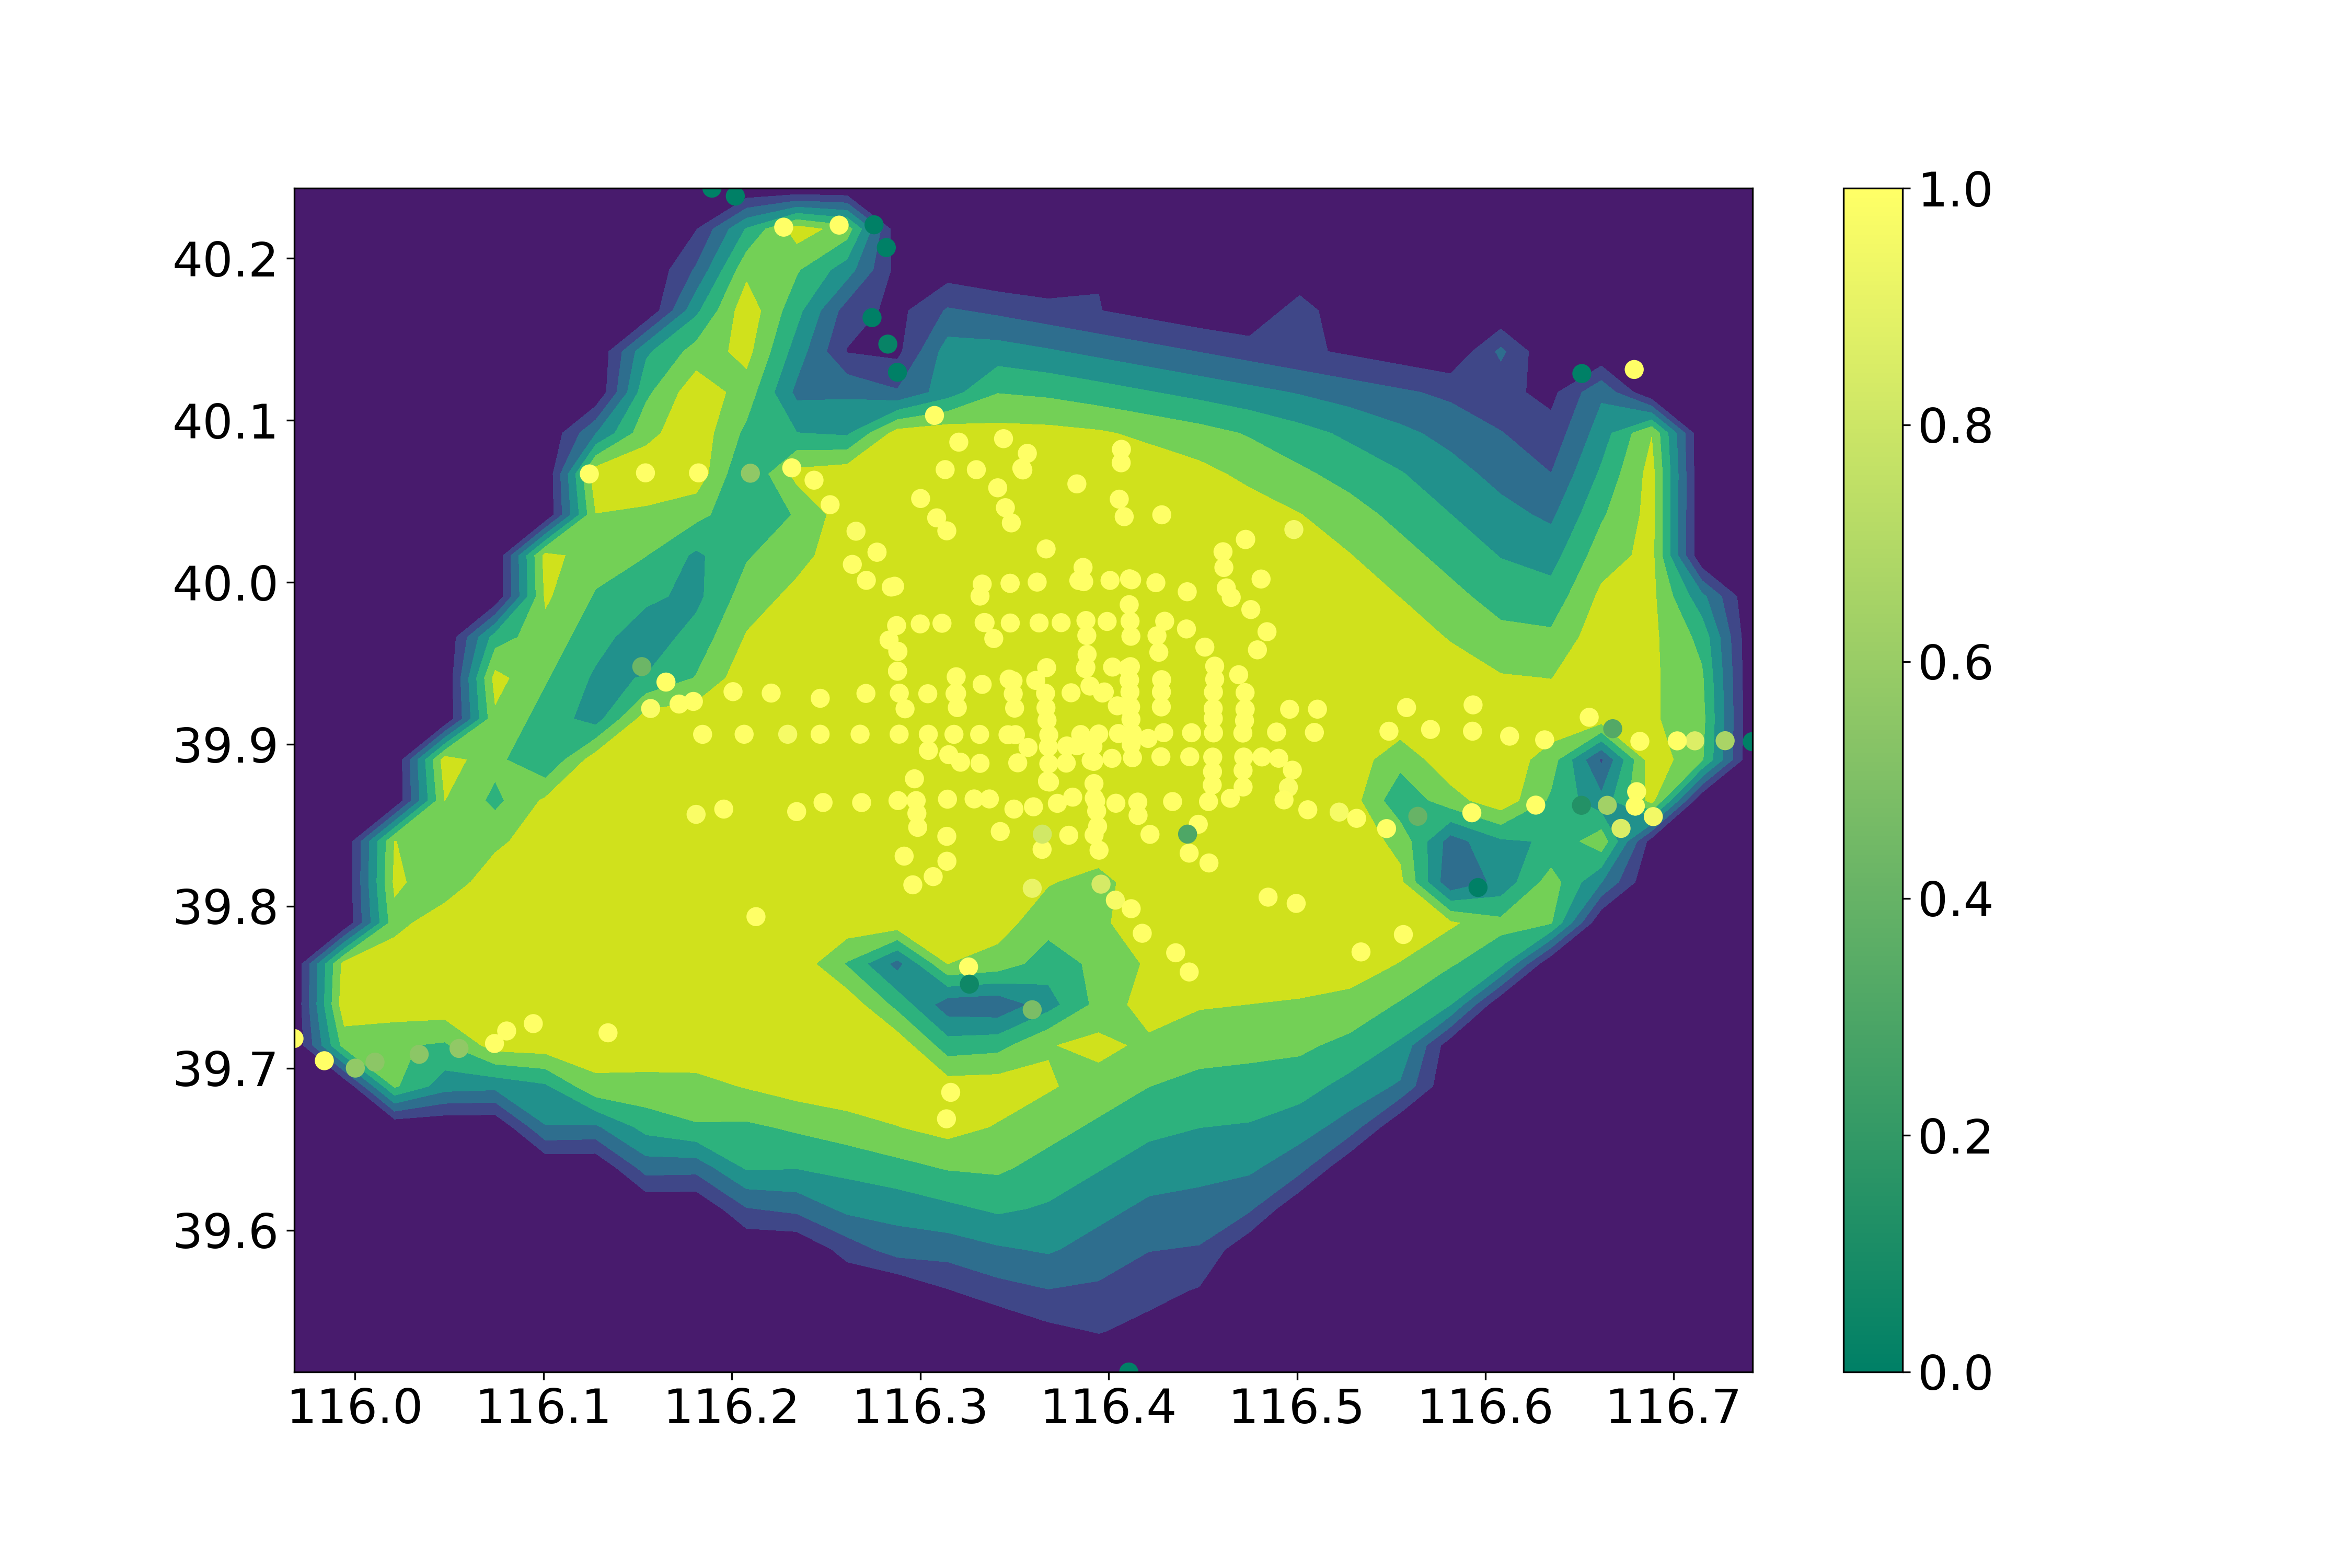
\includegraphics[width=\linewidth]{subway_coverages_0,00333333_lambda_heatmap.png}
		\caption{Mappa di calore ottenuta per $\lambda = 1/300$}
	\end{subfigure}
	\caption[Risultati metropolitana, $\lambda = 1/300$]{I risultati ottenuti applicando il modello alle uscite della metropolitana con $\lambda = 1/300$}
	\label{fig:subway_coverage2}
\end{figure}

\begin{figure}[H]
	\centering
	\begin{subfigure}[b]{\linewidth}
		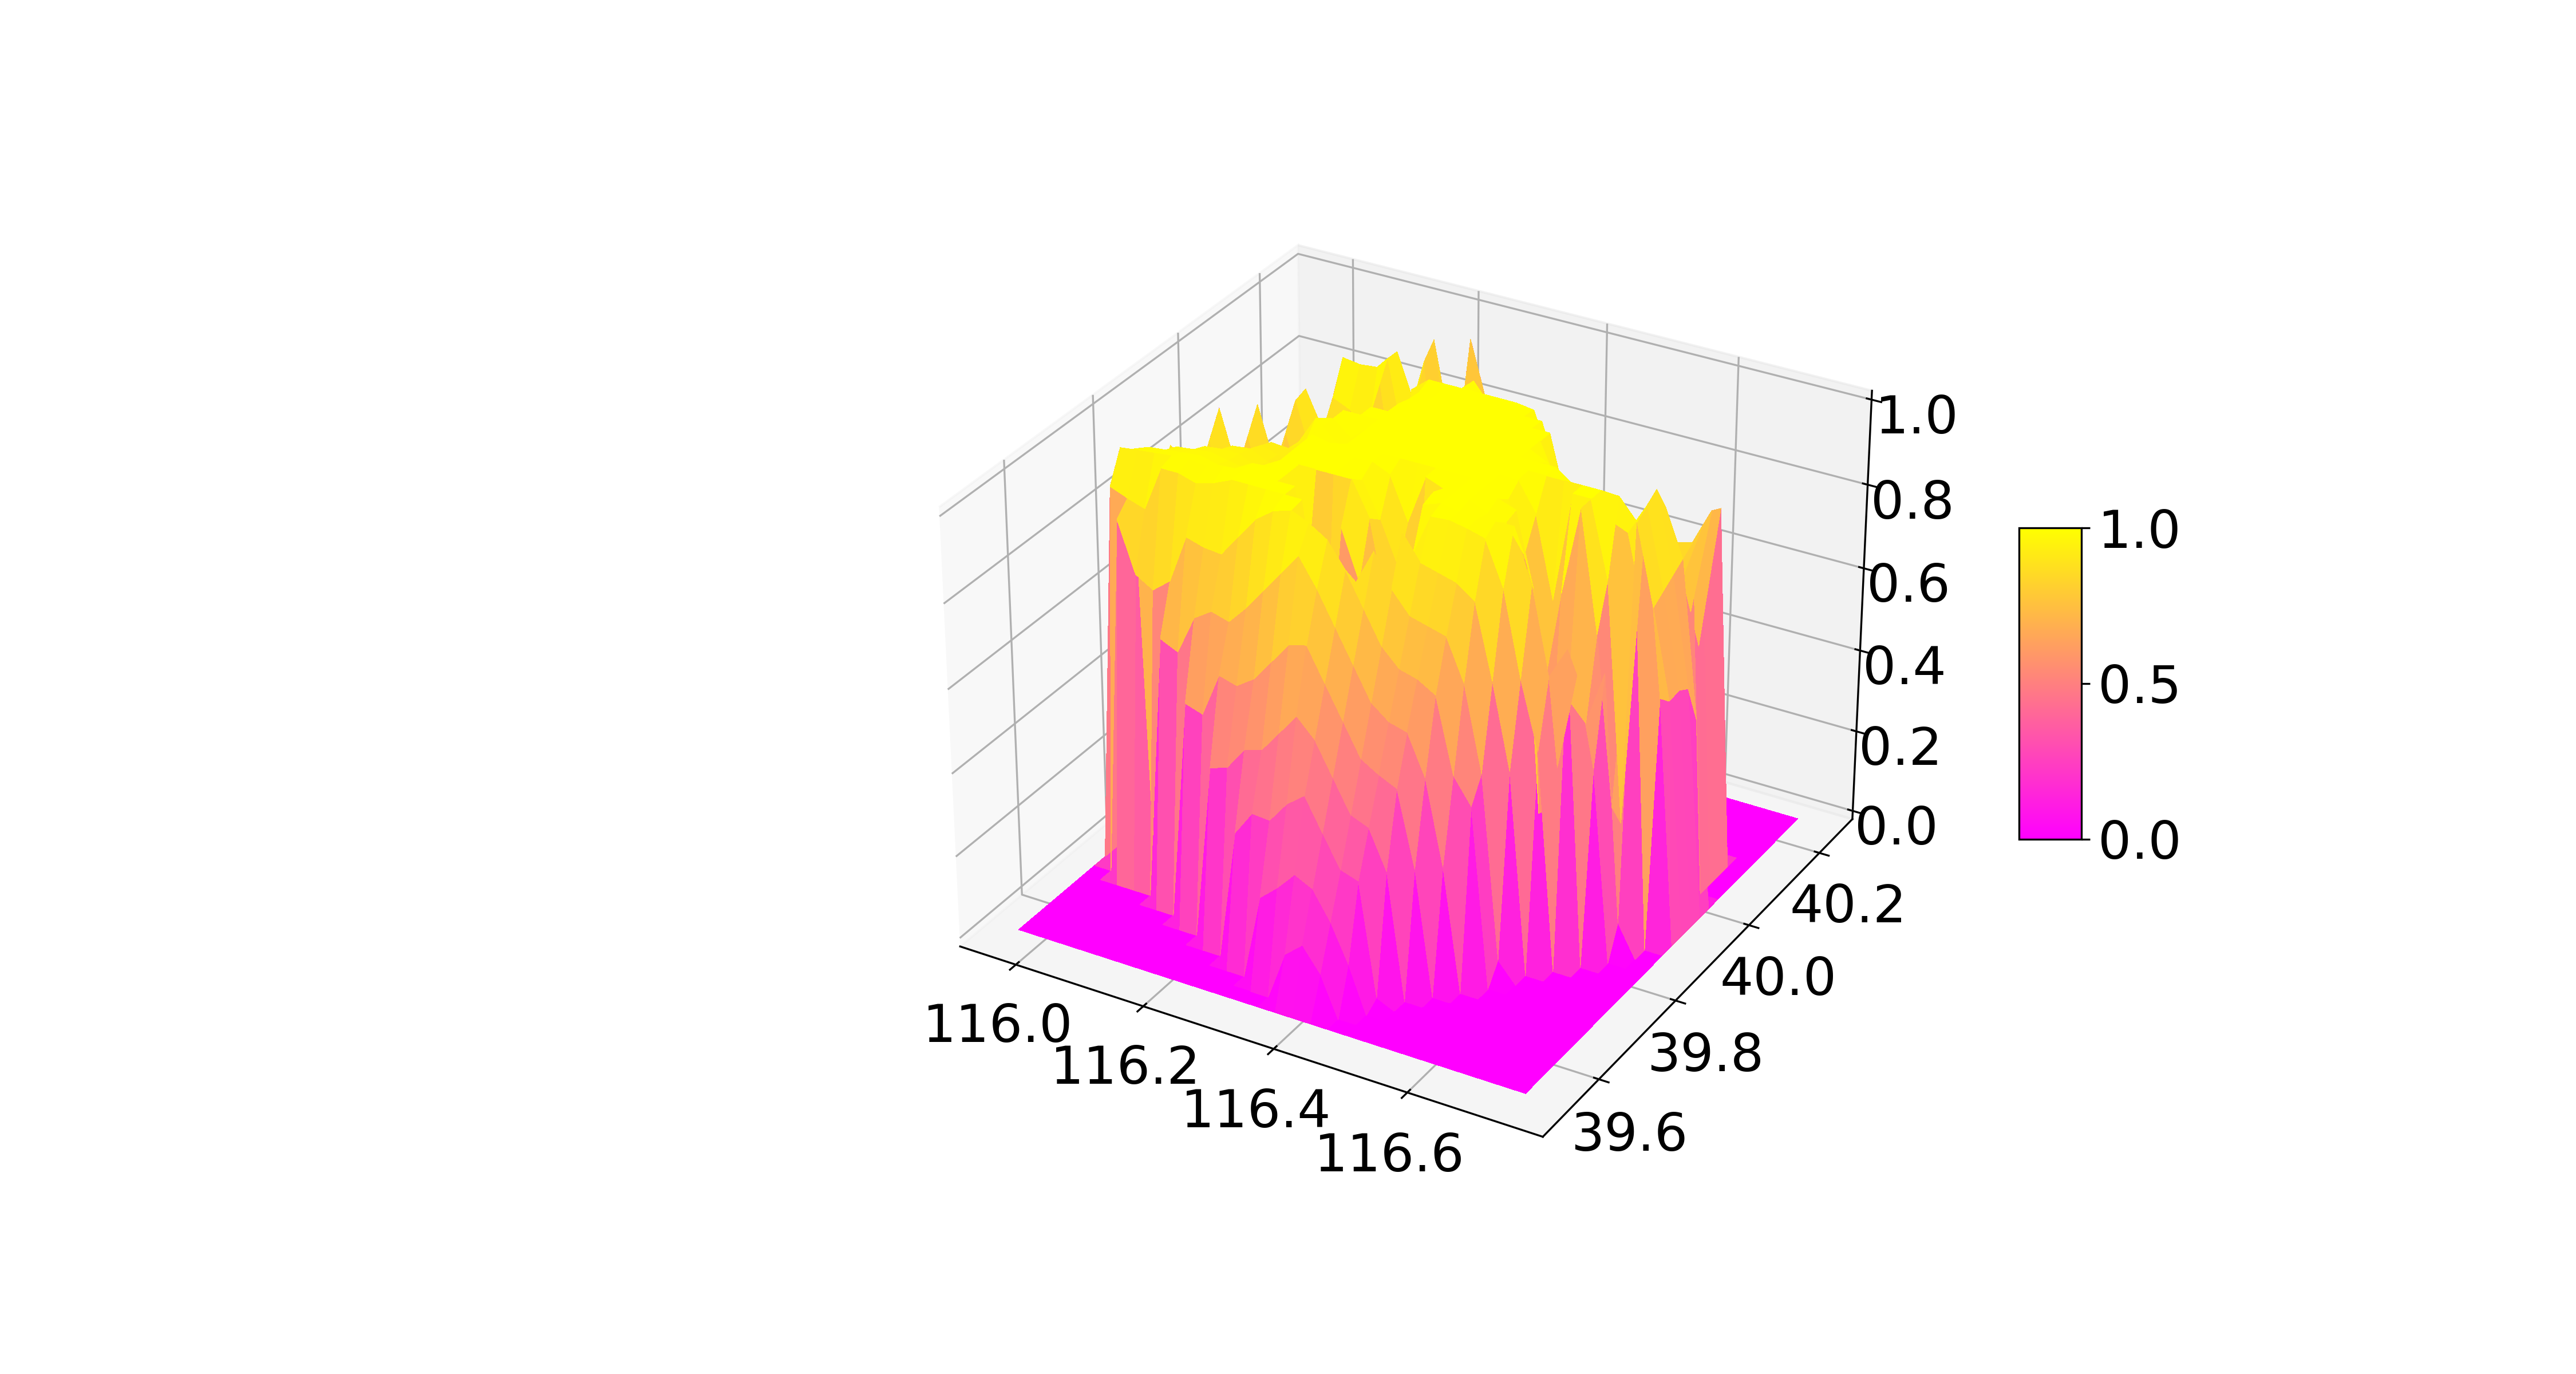
\includegraphics[width=\linewidth]{subway_coverages_0,00142857_lambda_3D_grid.png}
		\caption{Meshgrid ottenuta per $\lambda = 1/700$}
	\end{subfigure}
	\begin{subfigure}[b]{\linewidth}
		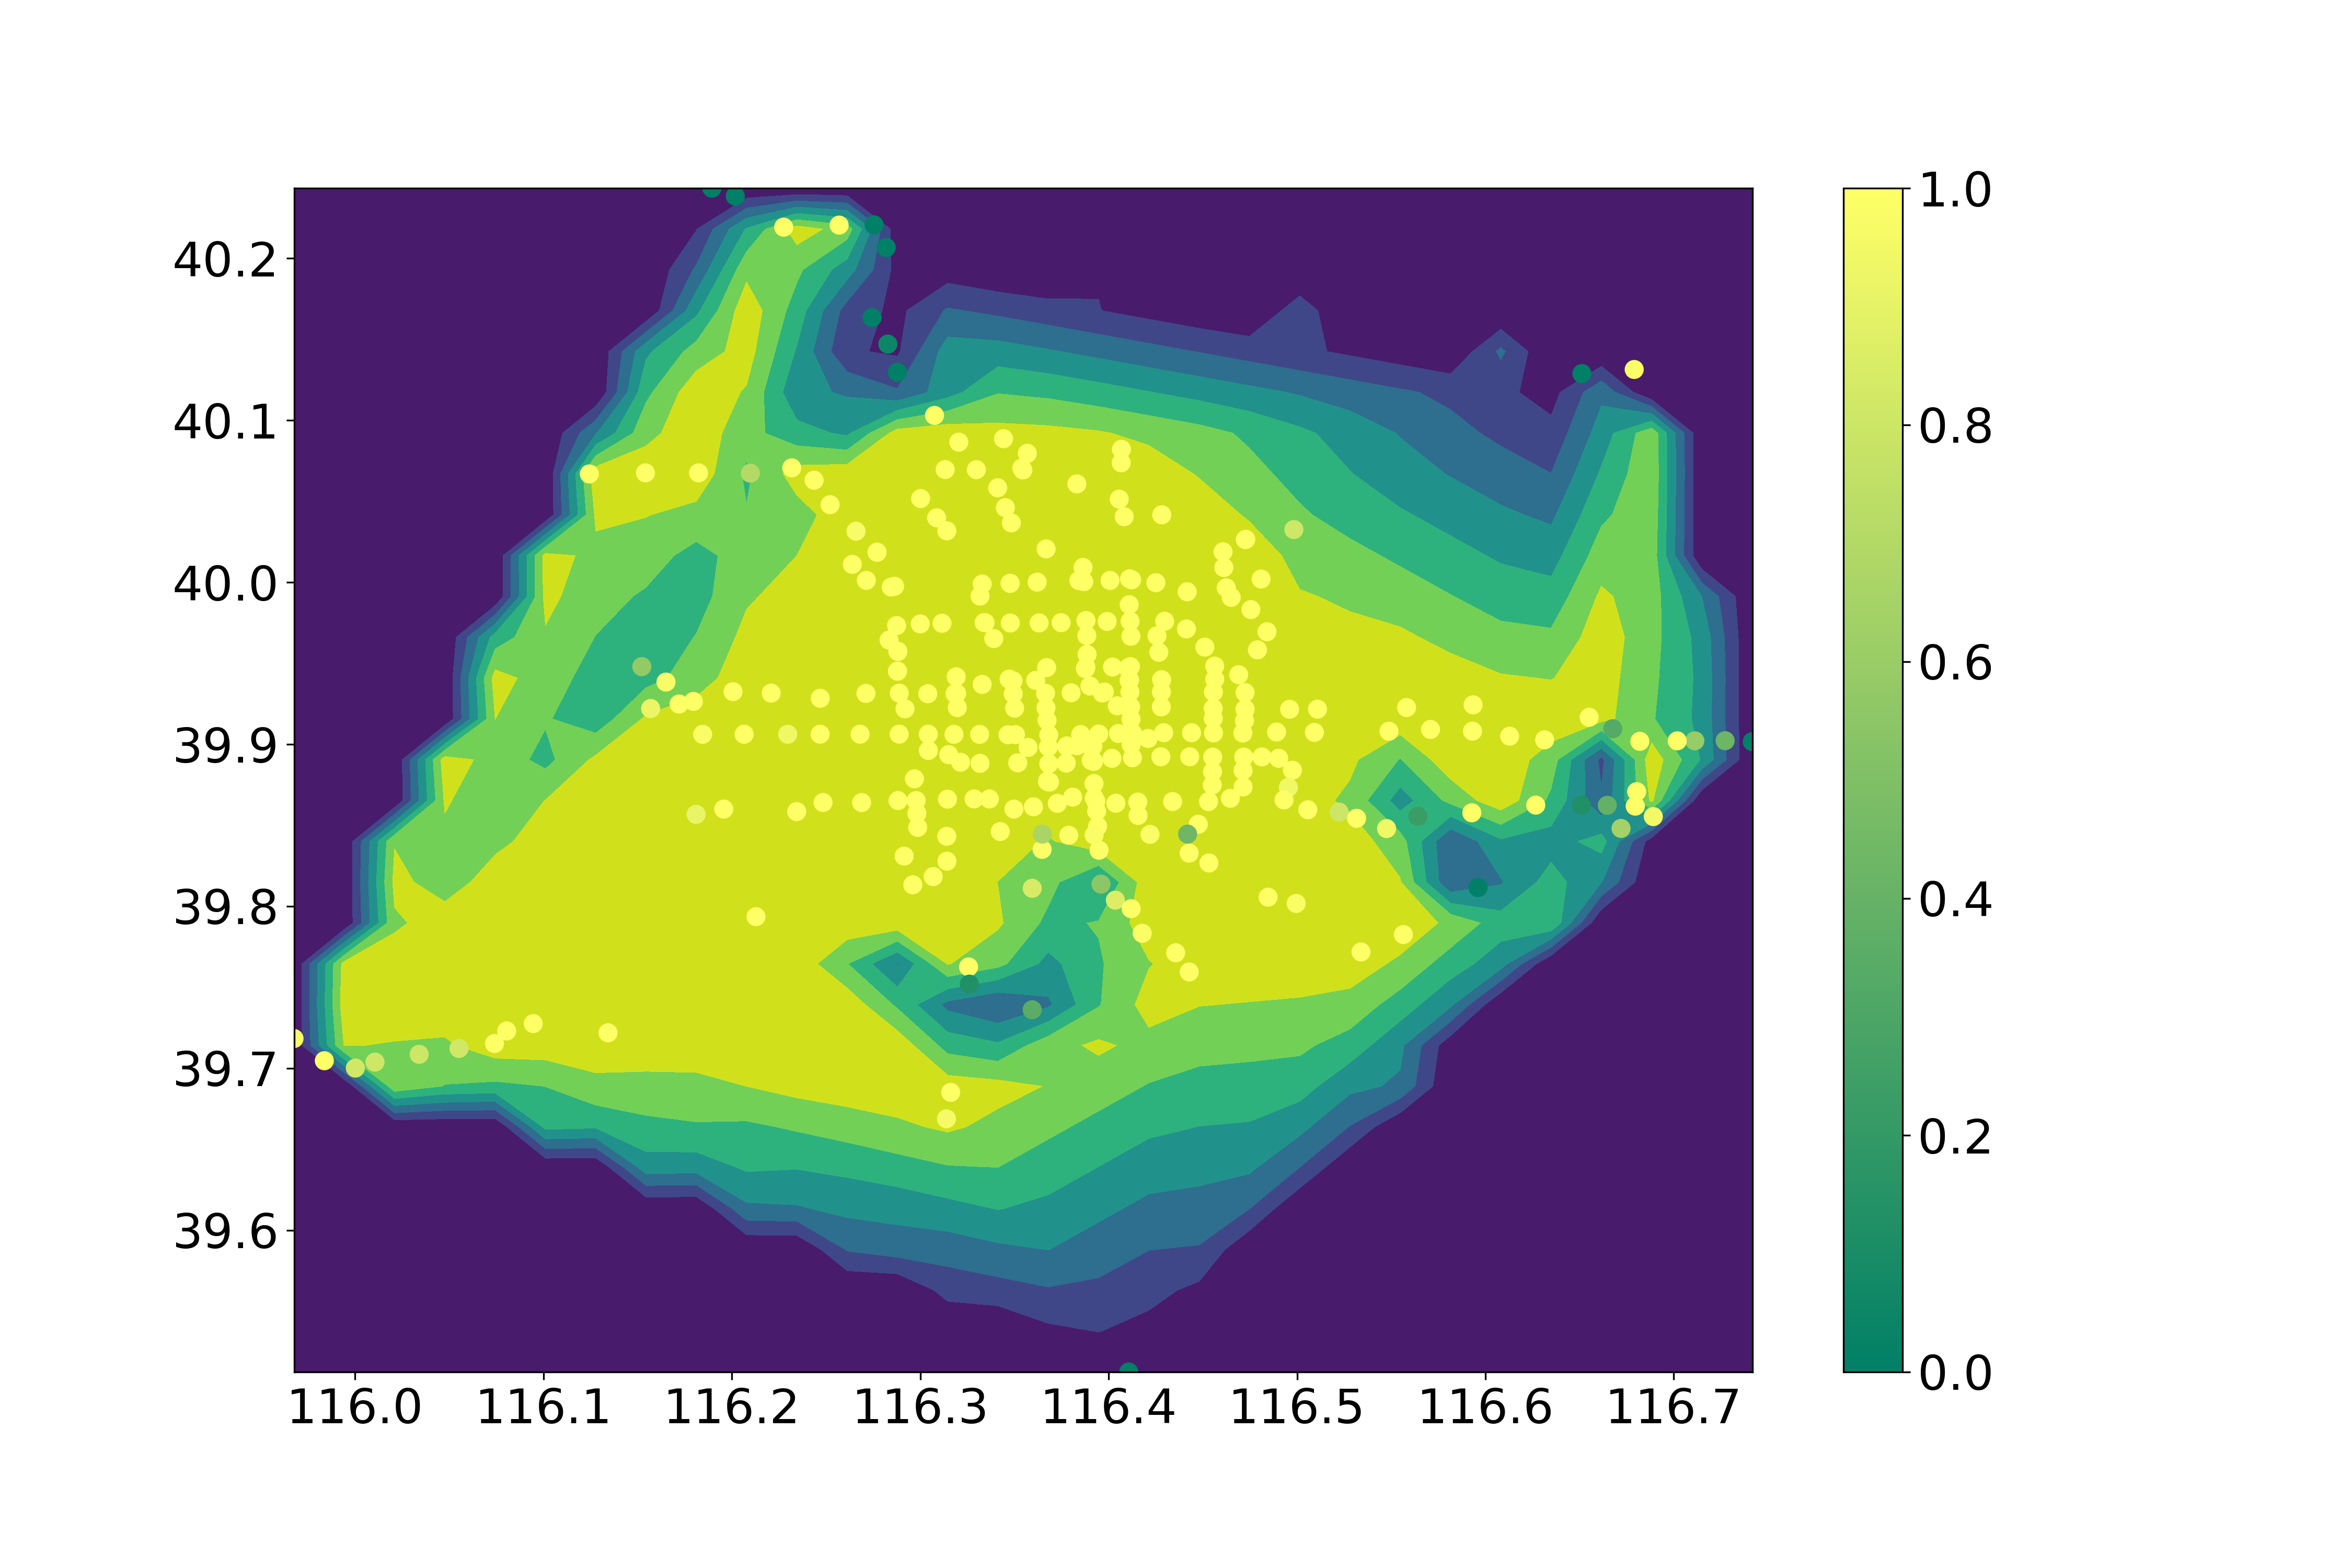
\includegraphics[width=\linewidth]{subway_coverages_0,00142857_lambda_heatmap.png}
		\caption{Mappa di calore ottenuta per $\lambda = 1/700$}
	\end{subfigure}
	\caption[Risultati metropolitana, $\lambda = 1/700$]{I risultati ottenuti applicando il modello alle uscite della metropolitana con $\lambda = 1/700$}
	\label{fig:subway_coverage3}
\end{figure}

\section{Punti di interesse}
I punti di interesse dislocati in tutta la città di Pechino ci permettono di verificare quanto e dove le persone siano più interessate ad andare.
Il data set dei punti di interesse è stato estratto utlizzando OSMnx analogamente a quello delle metropolitane.

Questo tipo di MCS ha un'utilità nel verificare quali siano i luoghi più popolari, e potrebbe essere interessante per studi di tipo turistico e culturale.
\subsection{Punti di interesse considerati
}I punti che sono stati scelti sono tutti monumenti, piazze, edifici storici o luoghi di aggregazione sociale come ad esempio centri commerciali. 
Analogamente a quanto fatto con le uscite della metropolitana, abbiamo estratto le posizioni grazie a OSMnx \cite{osmnx} che permette un filtraggio a grana fine basato su tags per trovare determinate tipologie di punti di interesse.

Dopo la pulizia abbiamo serializzato il dataset, contentente un totale di 956 punti di interesse sparsi in tutta la città.

La Figura \ref{fig:POI} mostra i punti di interesse presi in considerazione, stampati per mezzo di folium \cite{folium}.
Anche in questo caso i cerchi blu rappresentano le singole locazioni e in sovraimpressione sono presenti alcune delle traiettorie di Augmented Geolife.

\begin{figure}[H]
	\centering 
	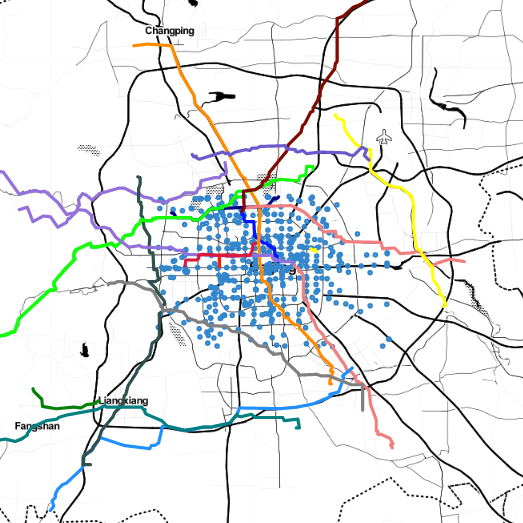
\includegraphics[width=\linewidth]{POI_folium.png}
	\caption[Mappa dei punti di interesse]{I punti di interesse estratti visualizzati grazie a folium}
	\label{fig:POI}
\end{figure}


\subsection{Risultati del modello di coverage}
Le Figure \ref{fig:POIs_coverage1}, \ref{fig:POIs_coverage2}, e \ref{fig:POIs_coverage3}, mostrano i risultati ottenuti applicando il modello con differenti valori di lambda sui punti di interesse estratti per mezzo di OSMnx \cite{osmnx}. 

\newpage

\begin{figure}[H]
	\centering
	\begin{subfigure}[b]{\linewidth}
		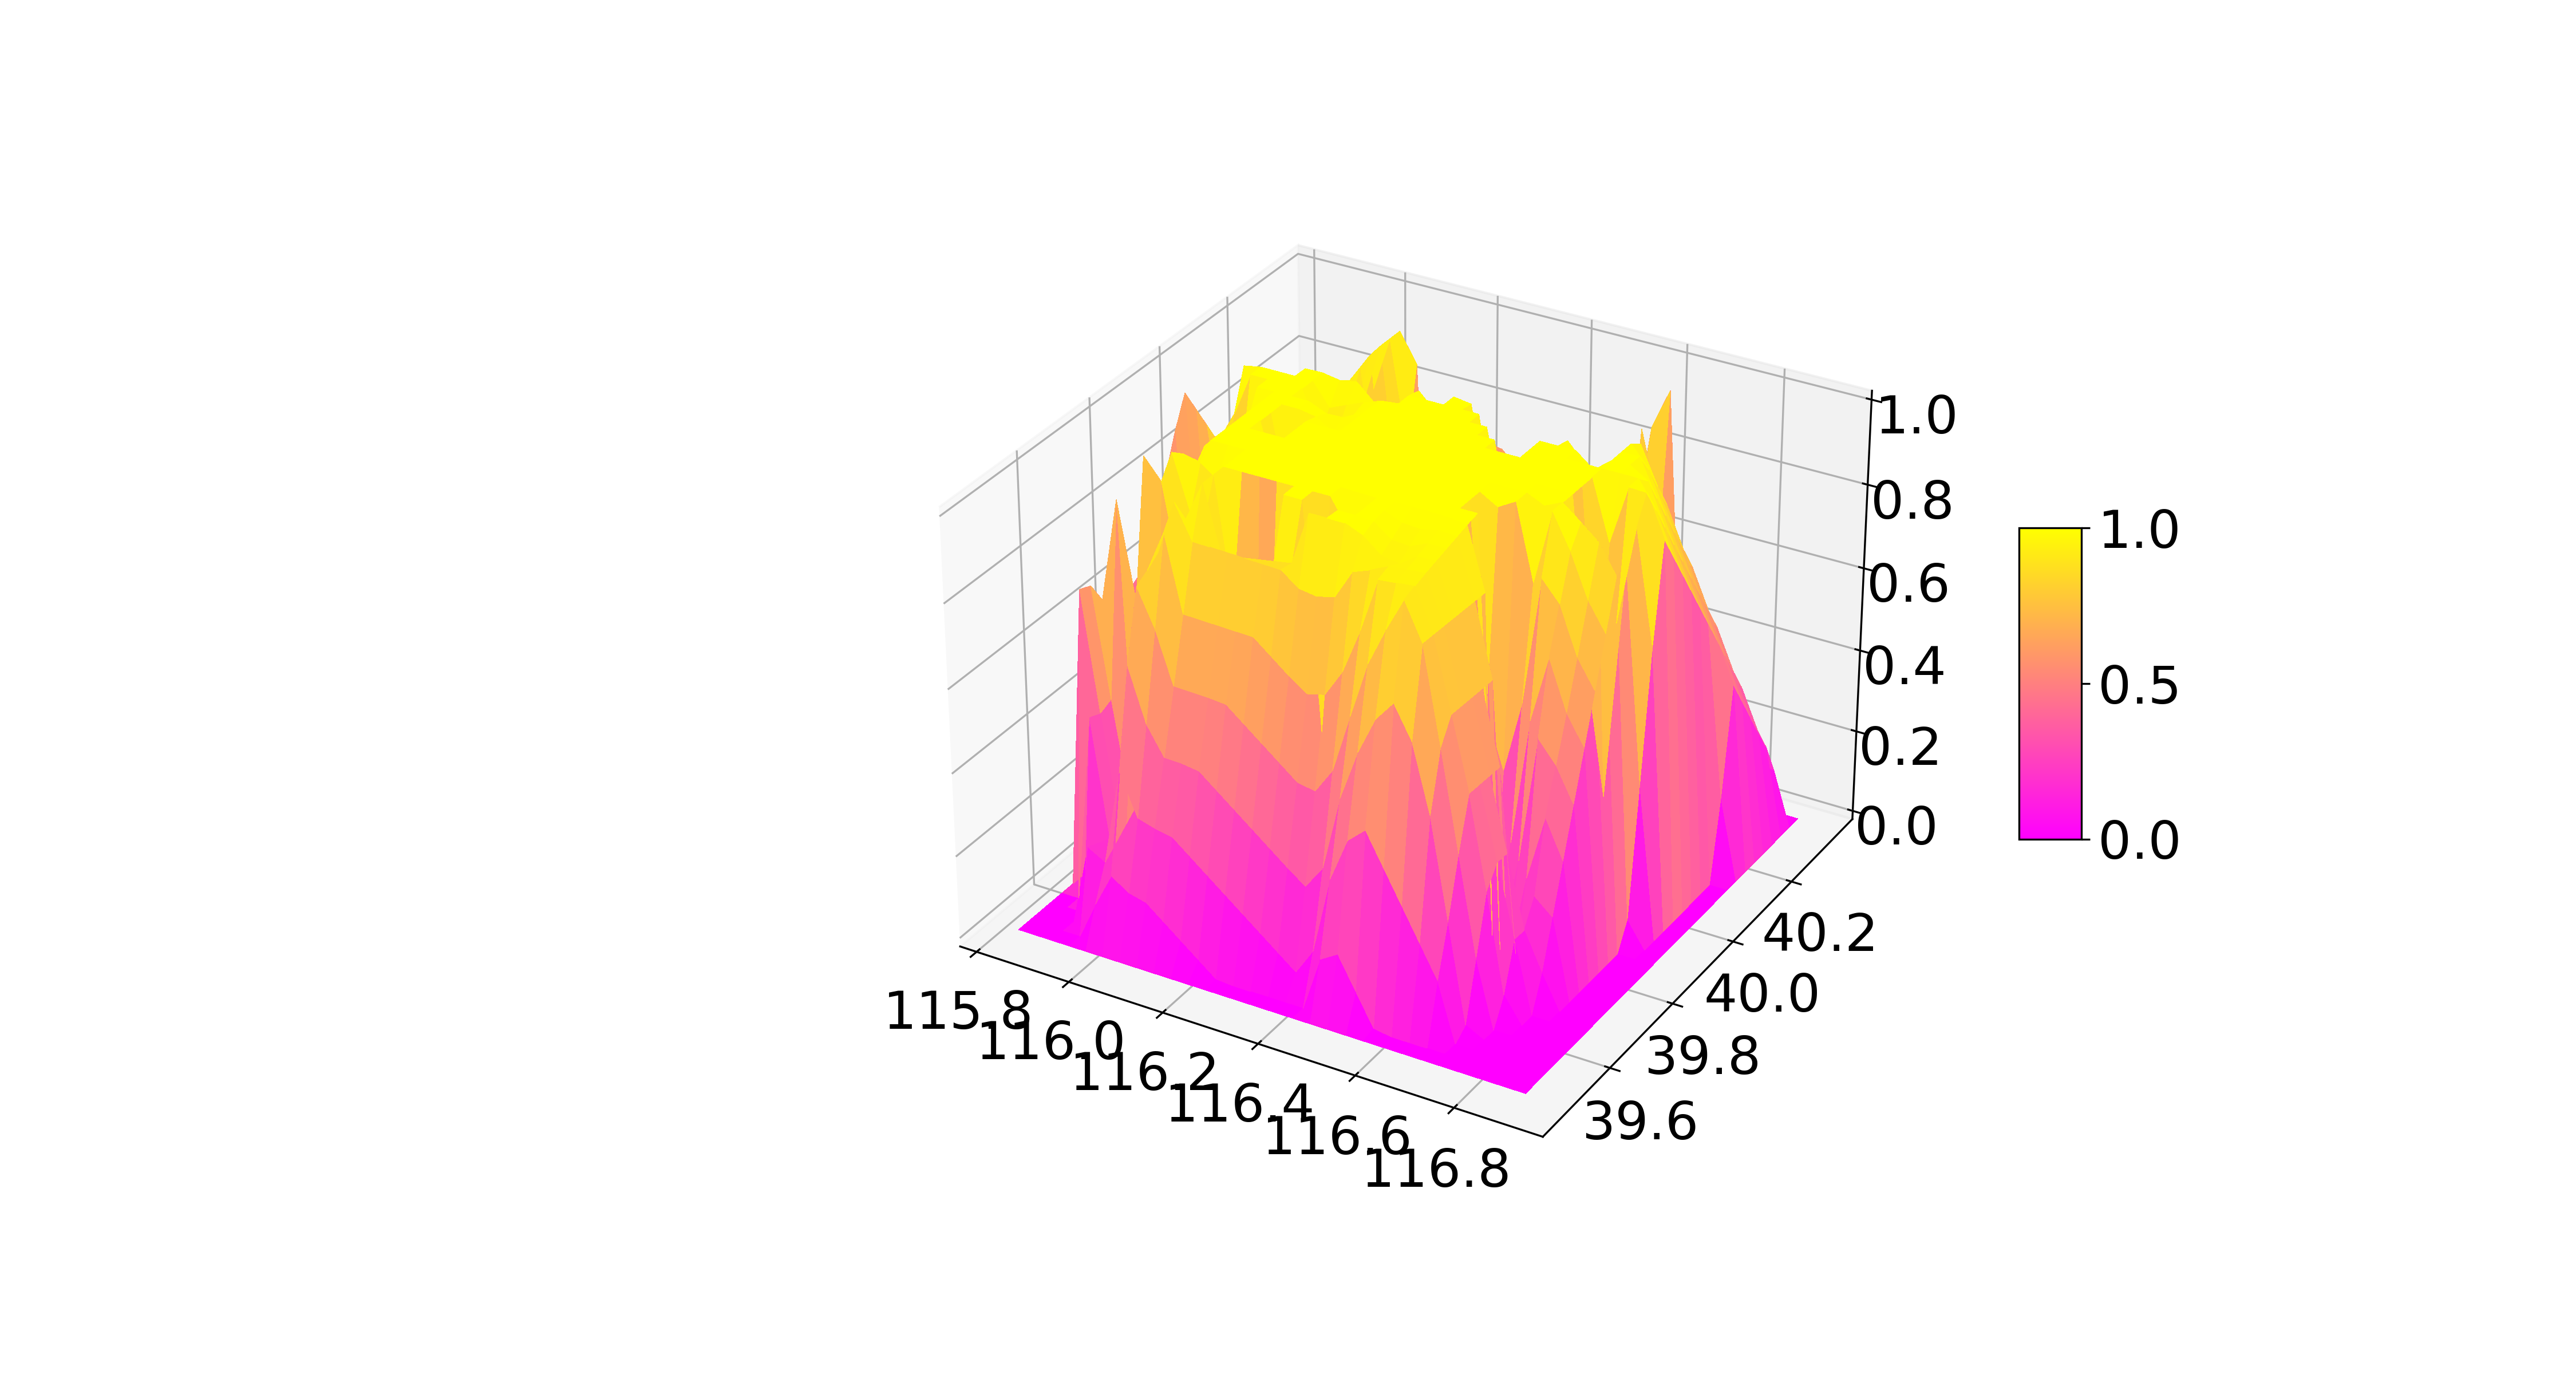
\includegraphics[width=\linewidth]{POIs_coverages_0,01_lambda_3D_grid.png}
		\caption{Meshgrid ottenuta per $\lambda = 1/100$}
	\end{subfigure}
	\begin{subfigure}[b]{\linewidth}
		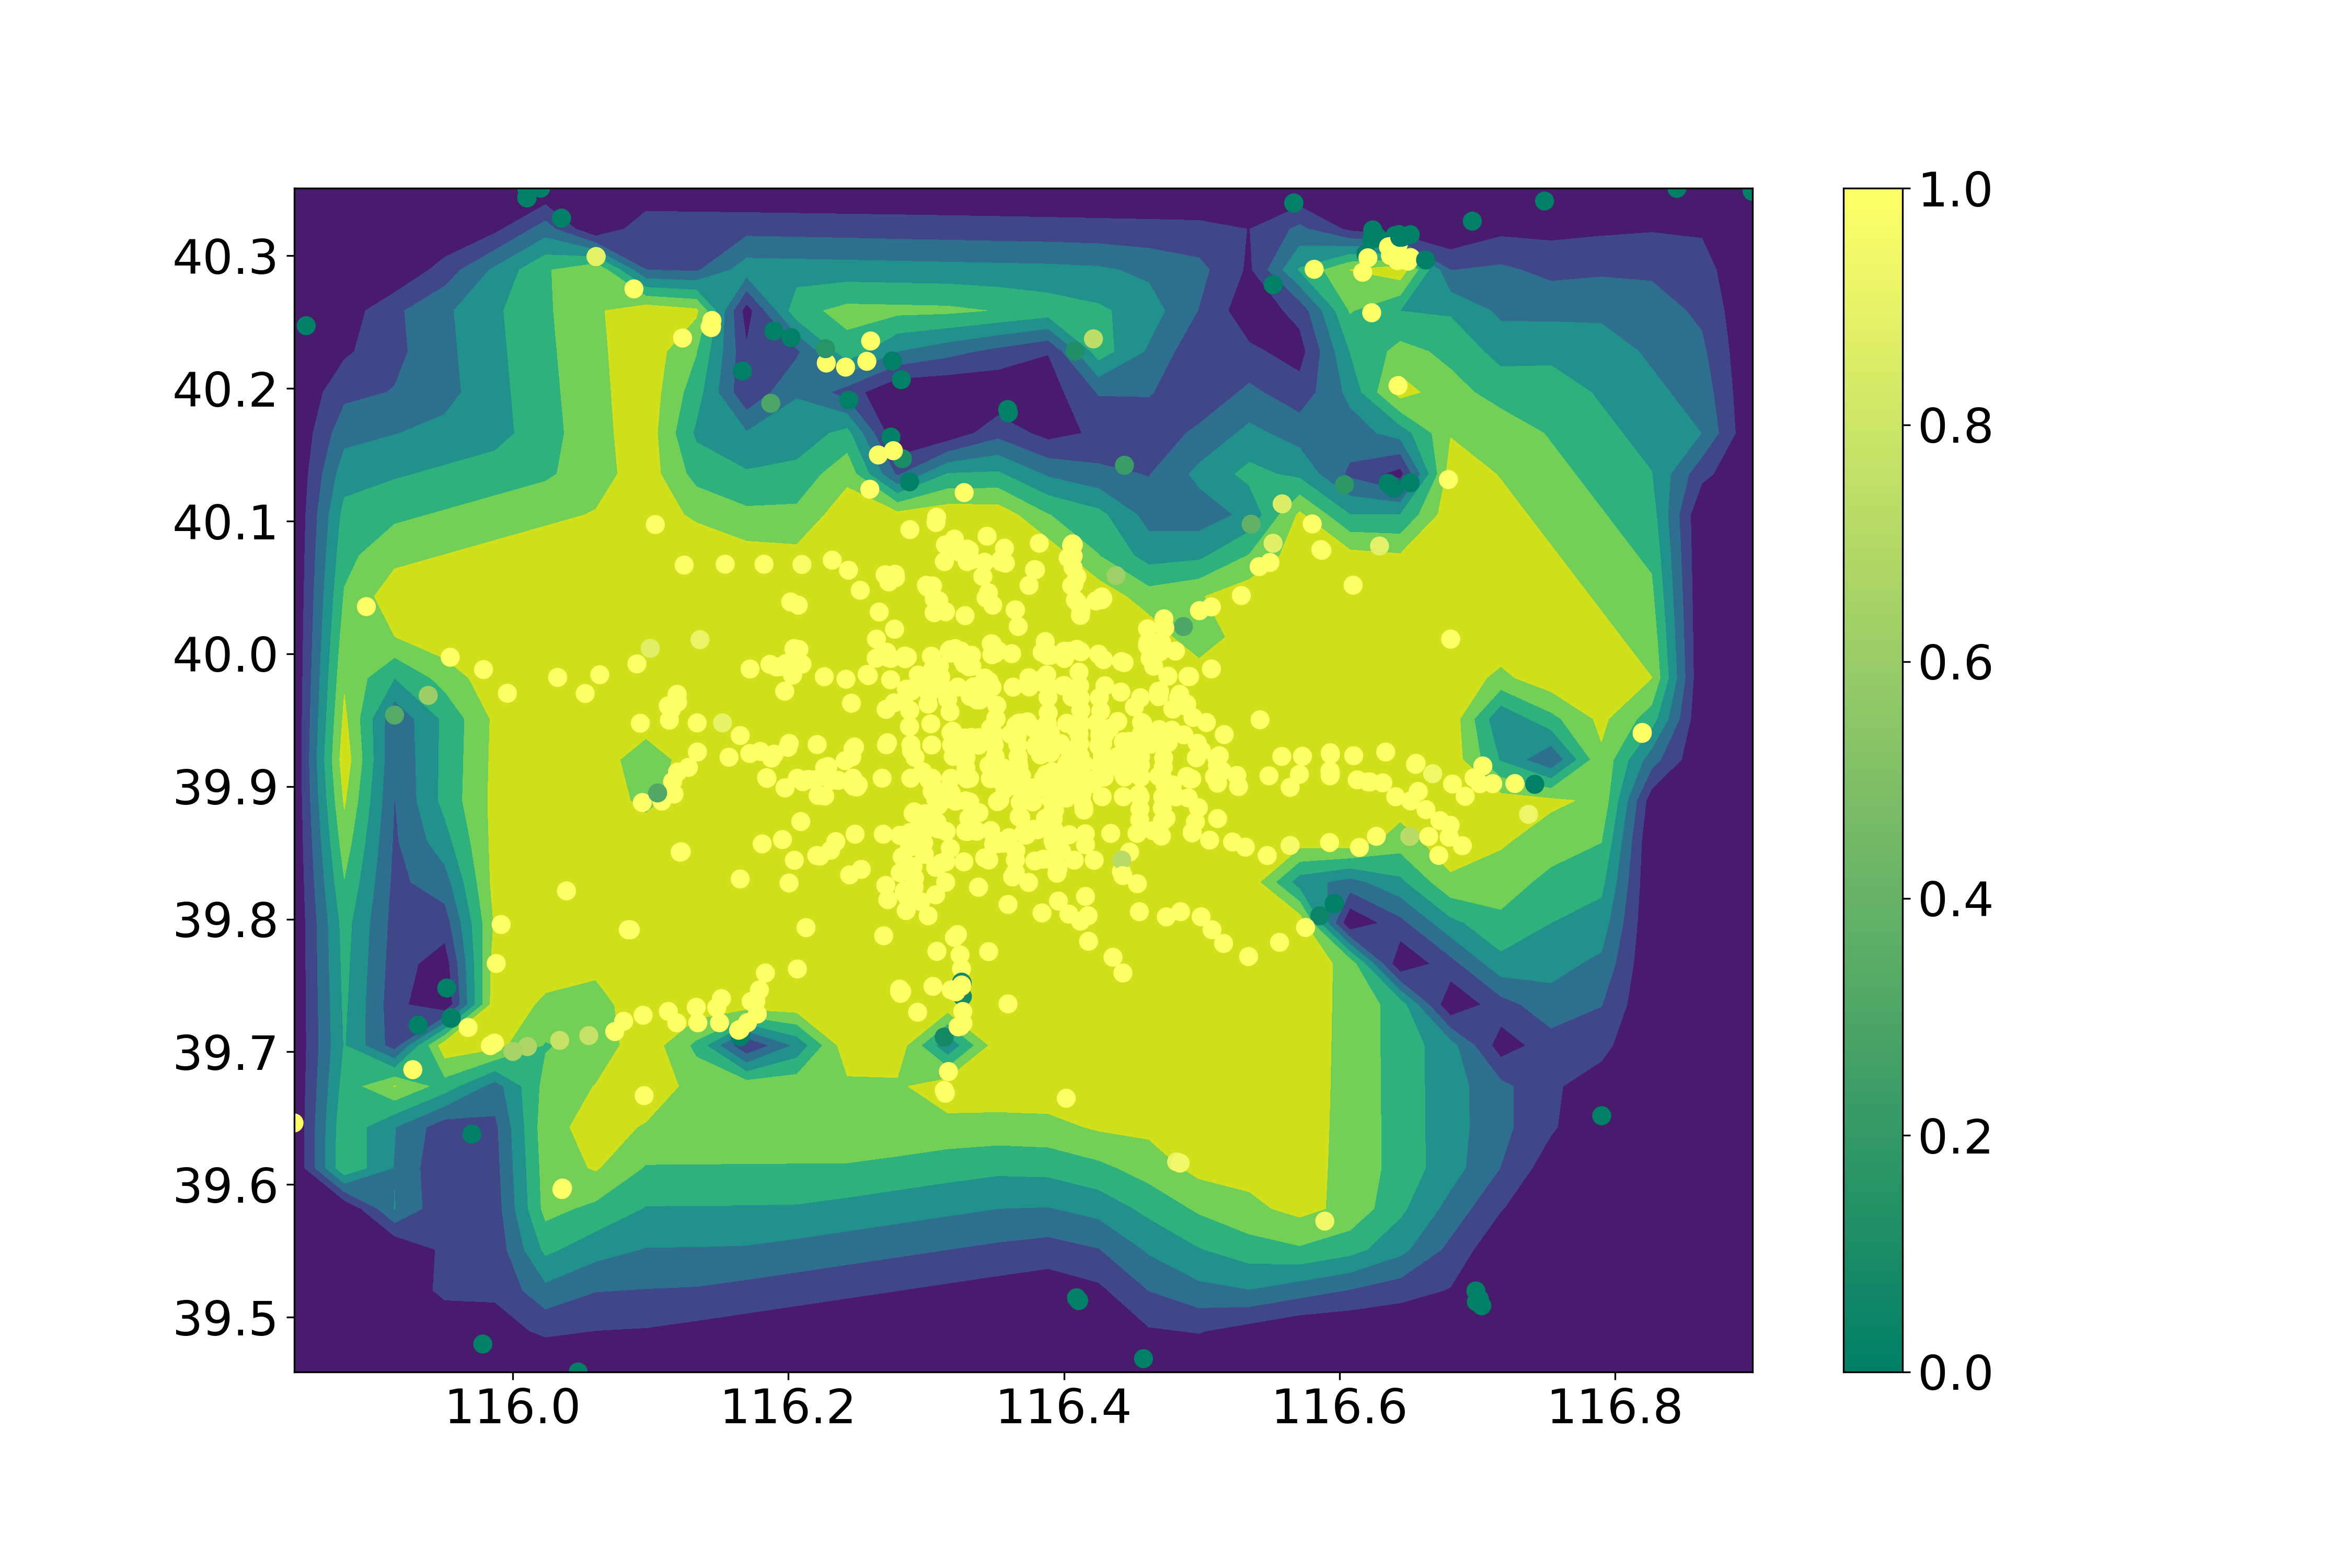
\includegraphics[width=\linewidth]{POIs_coverages_0,01_lambda_heatmap.png}
		\caption{Mappa di calore ottenuta per $\lambda = 1/100$}
	\end{subfigure}
	\caption[Risultati POIs, $\lambda = 1/100$]{I risultati ottenuti applicando il modello ai punti di interesse con $\lambda = 1/100$}
	\label{fig:POIs_coverage1}
\end{figure}

\begin{figure}[H]
	\centering
	\begin{subfigure}[b]{\linewidth}
		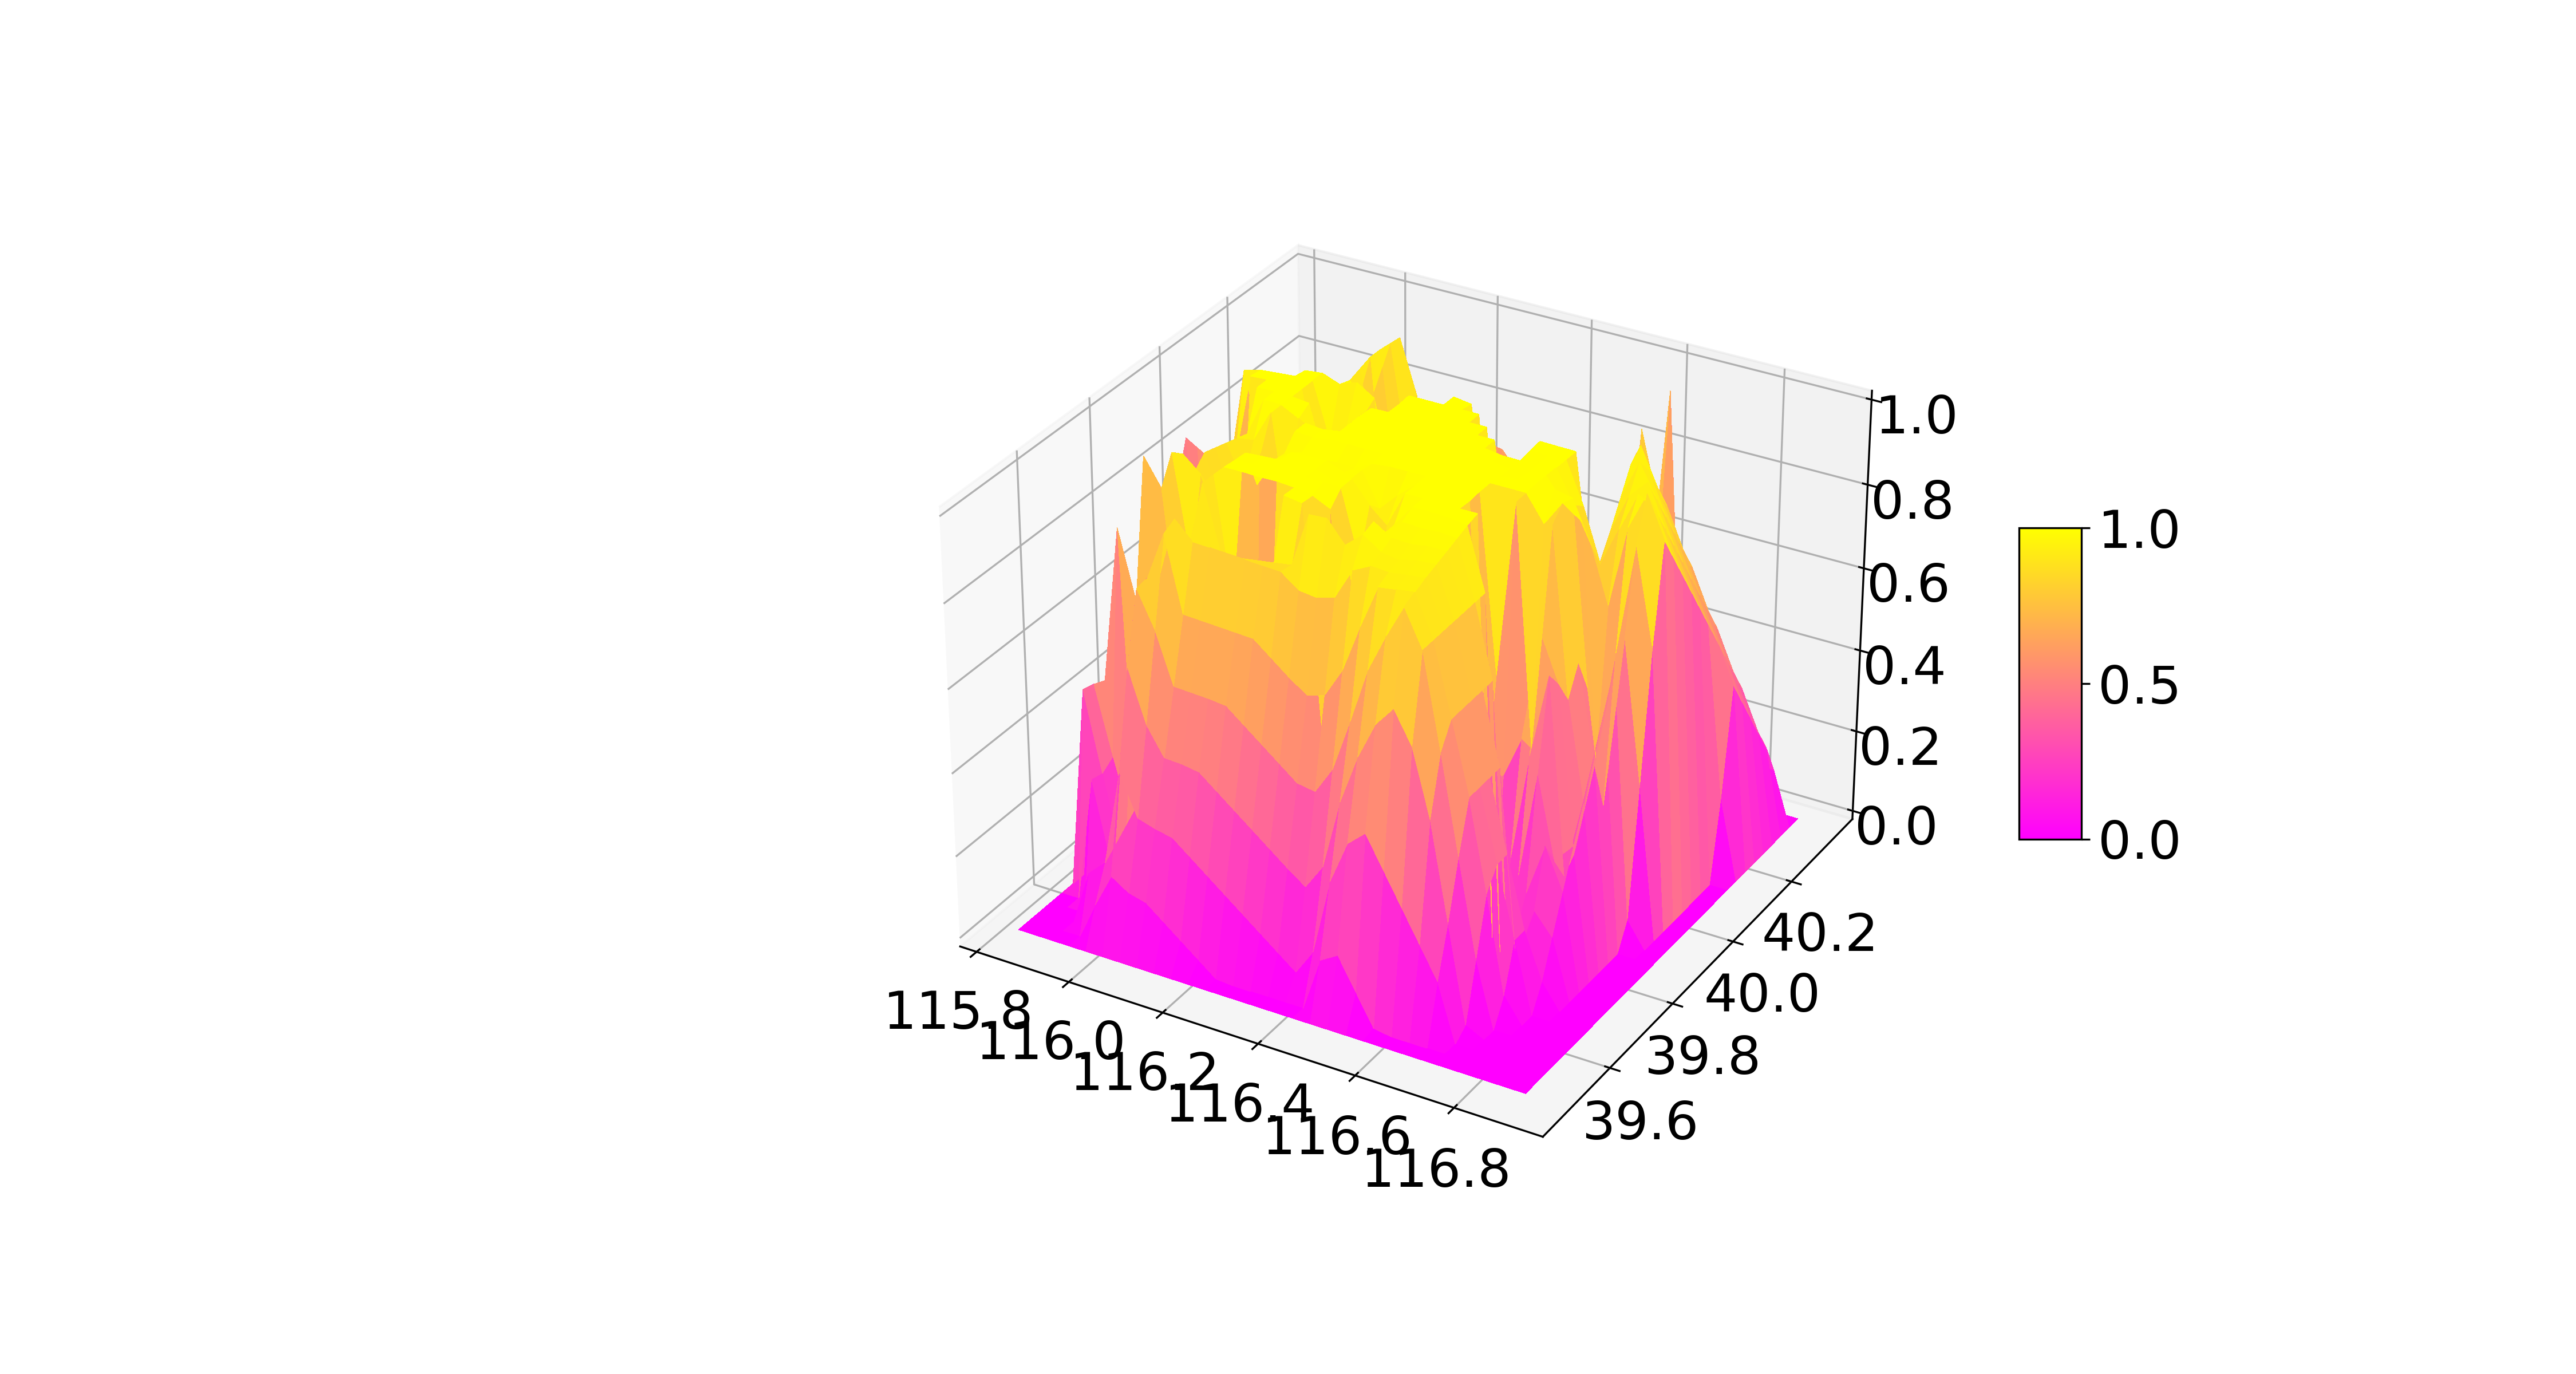
\includegraphics[width=\linewidth]{POIs_coverages_0,00333333_lambda_3D_grid.png}
		\caption{Meshgrid ottenuta per $\lambda = 1/300$}
	\end{subfigure}
	\begin{subfigure}[b]{\linewidth}
		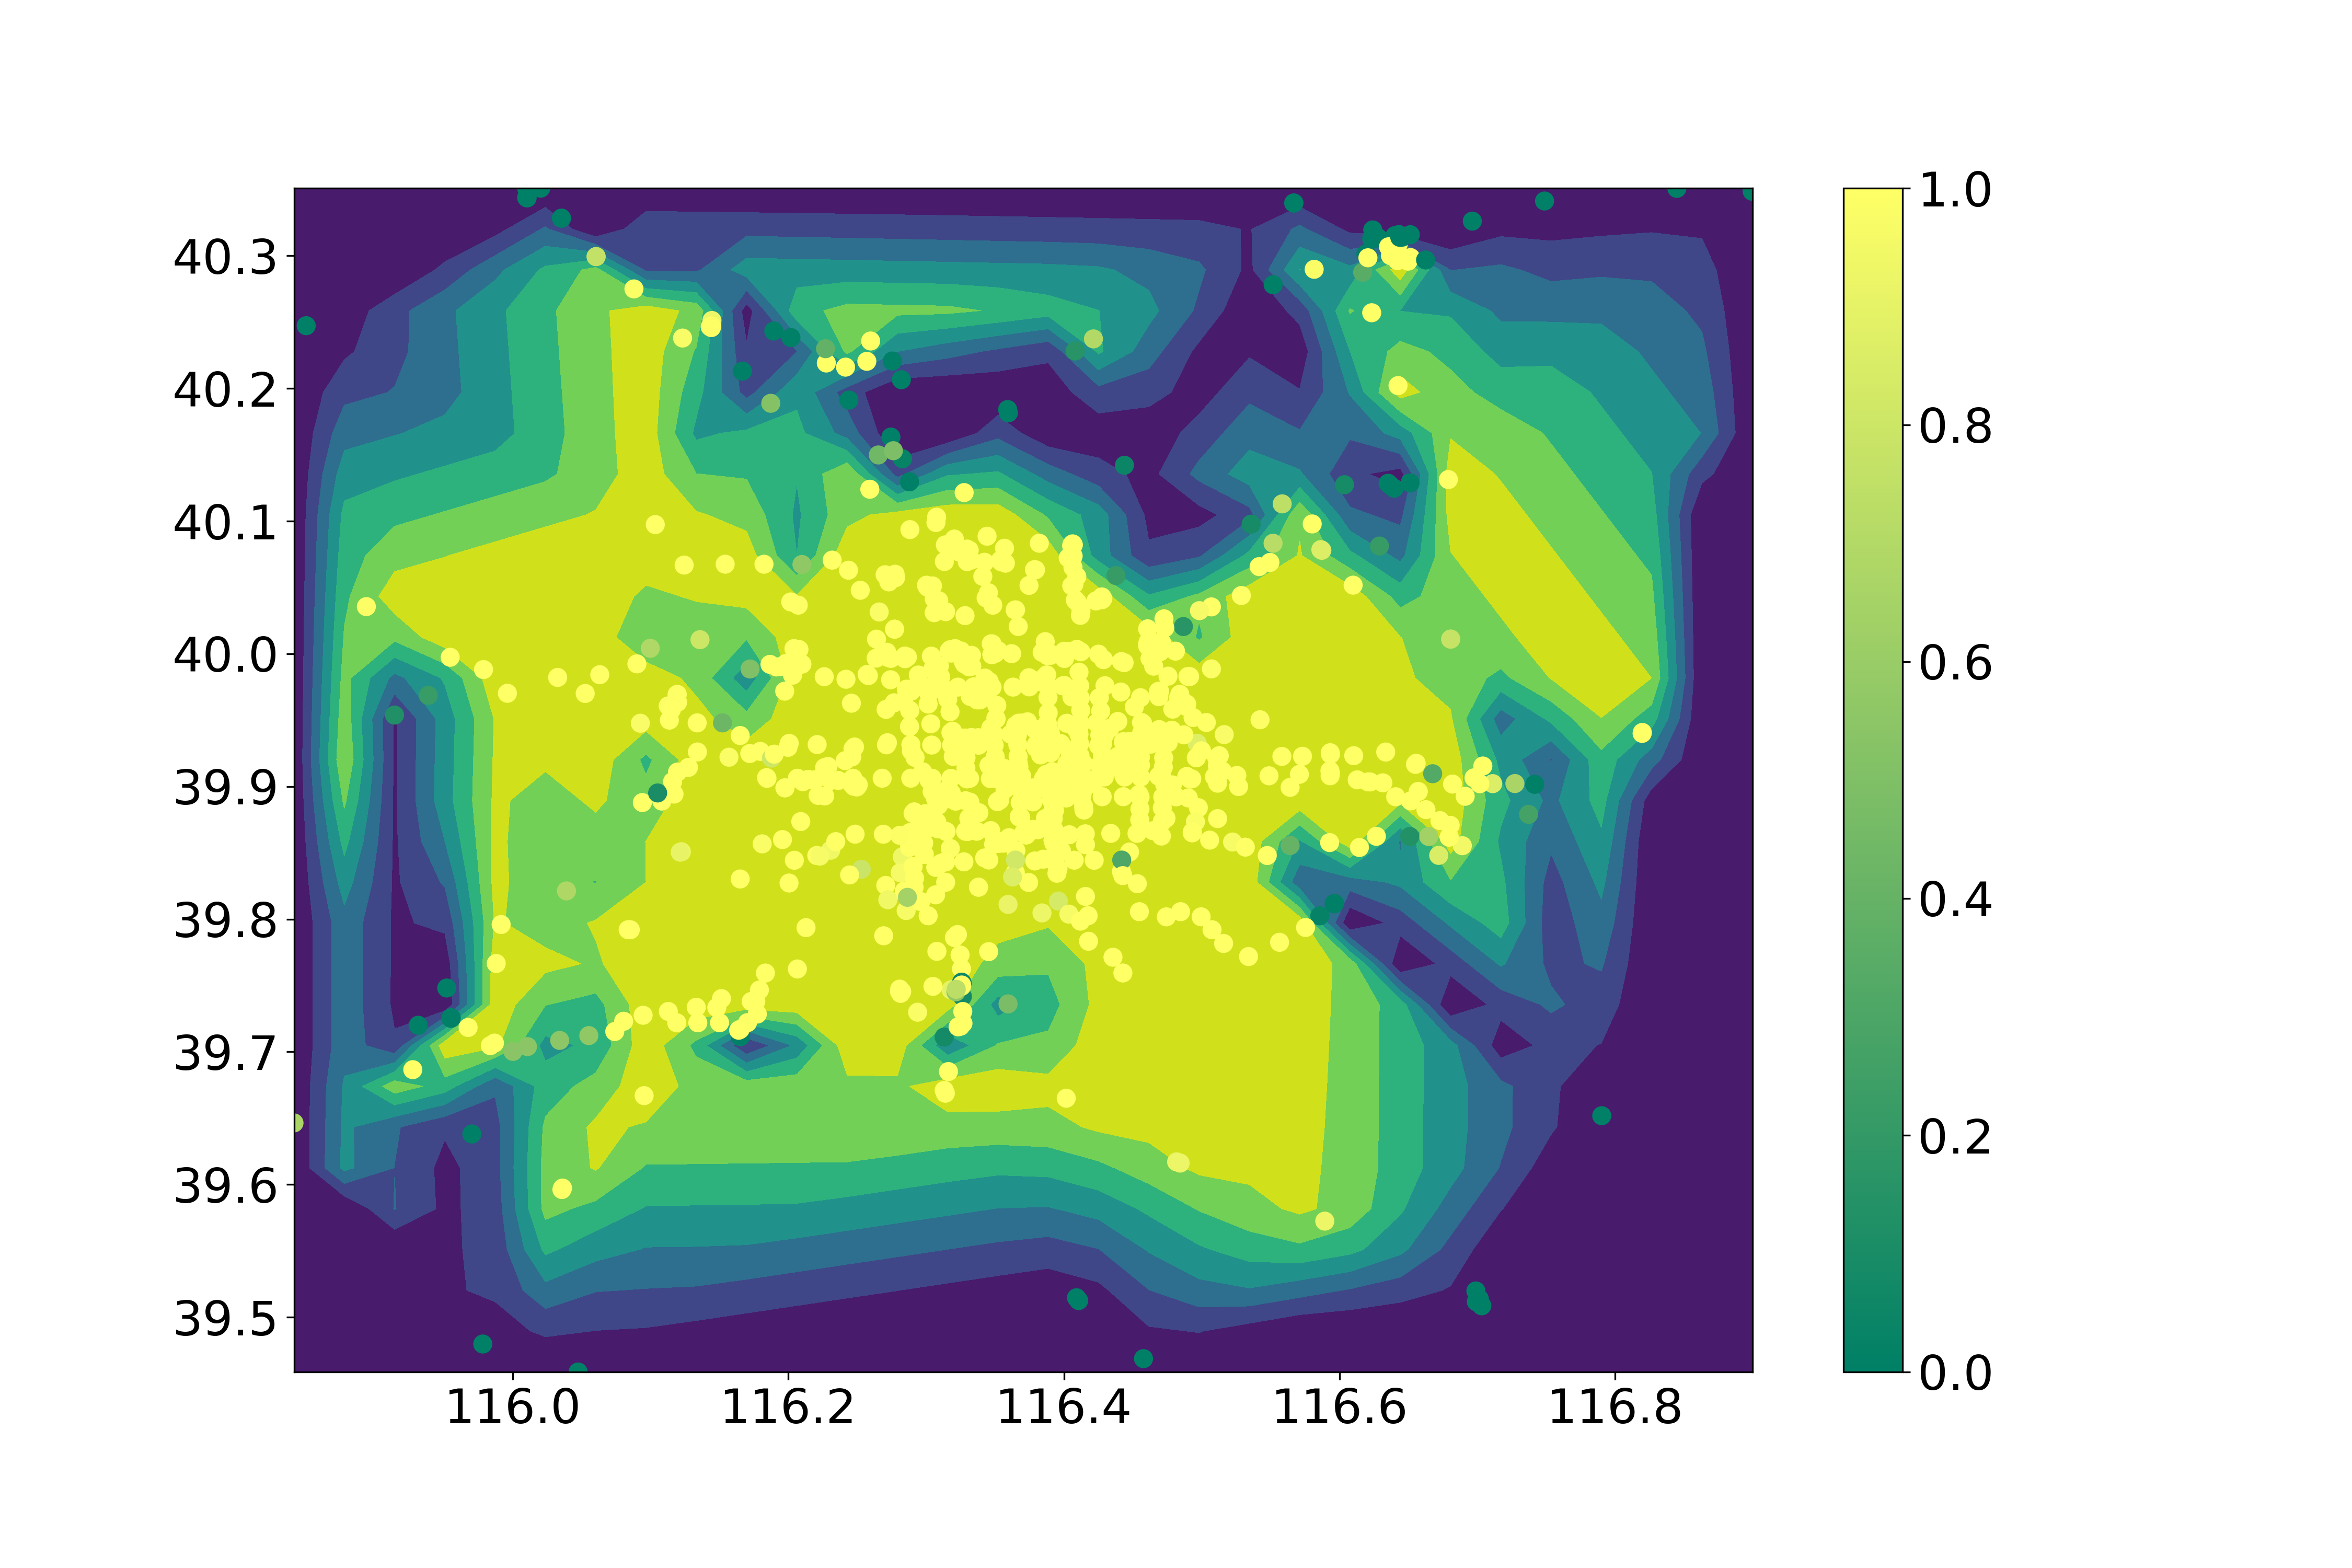
\includegraphics[width=\linewidth]{POIs_coverages_0,00333333_lambda_heatmap.png}
		\caption{Mappa di calore ottenuta per $\lambda = 1/300$}
	\end{subfigure}
	\caption[Risultati POIs, $\lambda = 1/300$]{I risultati ottenuti applicando il modello ai punti di interesse con $\lambda = 1/300$}
	\label{fig:POIs_coverage2}
\end{figure}

\begin{figure}[H]
	\centering
	\begin{subfigure}[b]{\linewidth}
		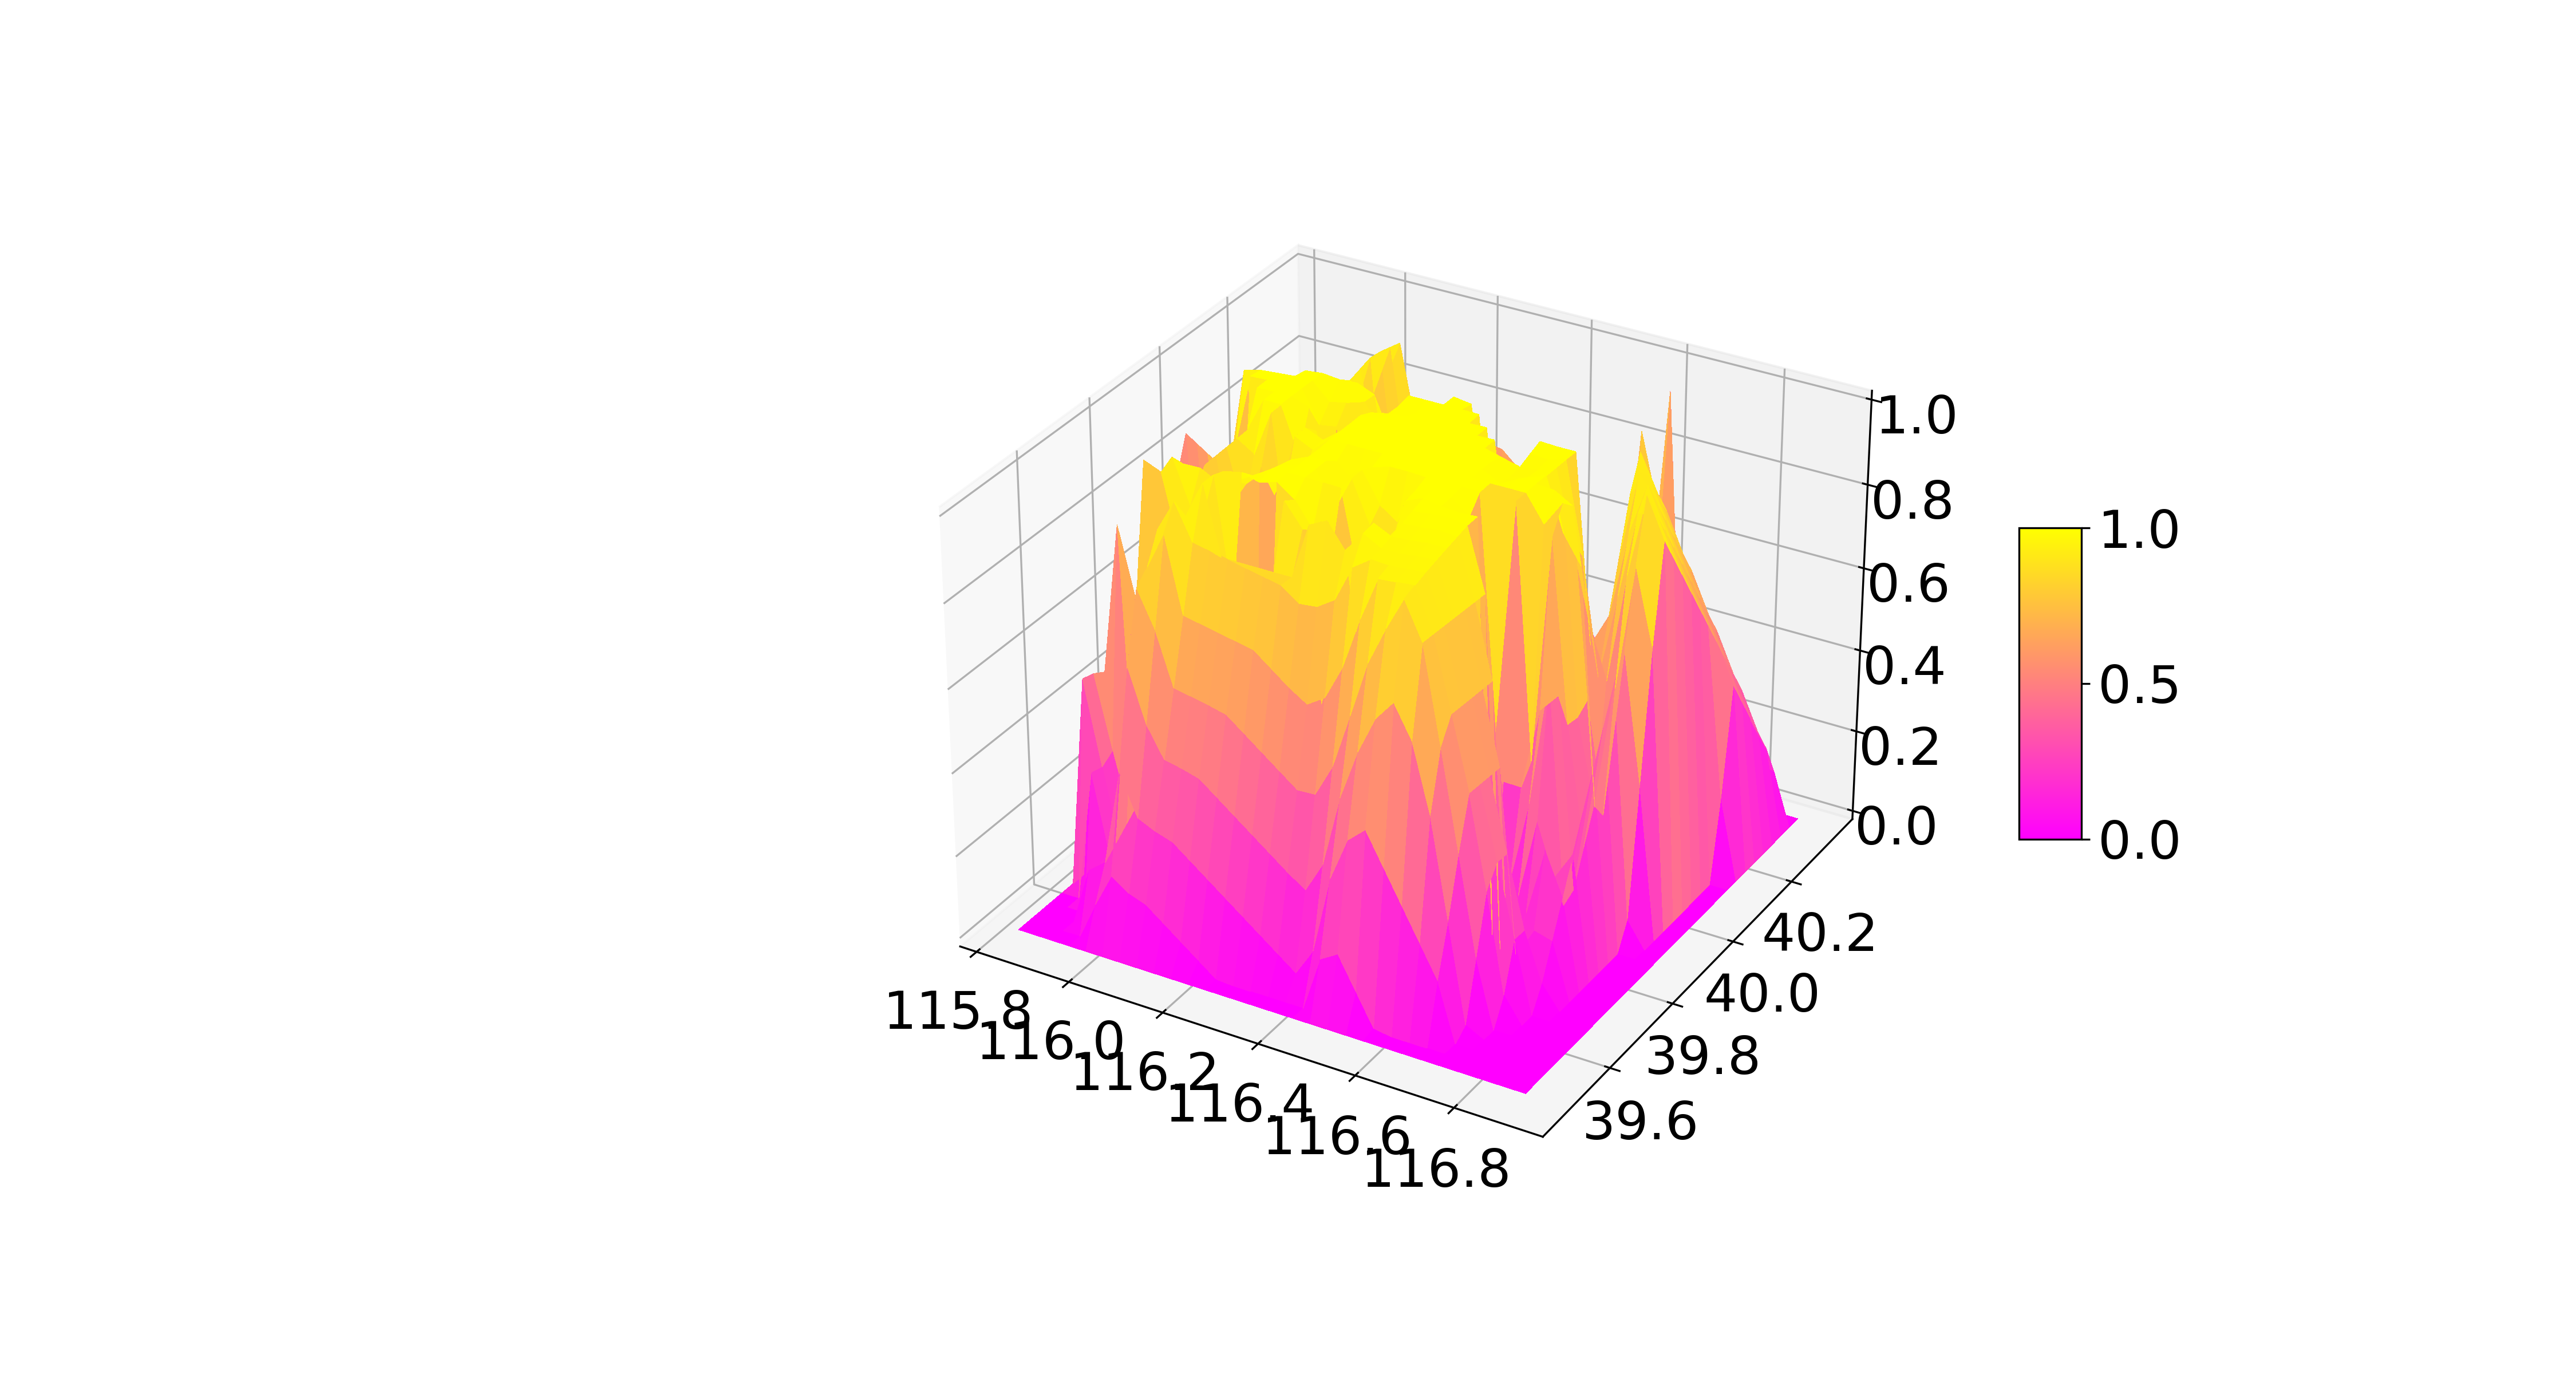
\includegraphics[width=\linewidth]{POIs_coverages_0,00142857_lambda_3D_grid.png}
		\caption{Meshgrid ottenuta per $\lambda = 1/700$}
	\end{subfigure}
	\begin{subfigure}[b]{\linewidth}
		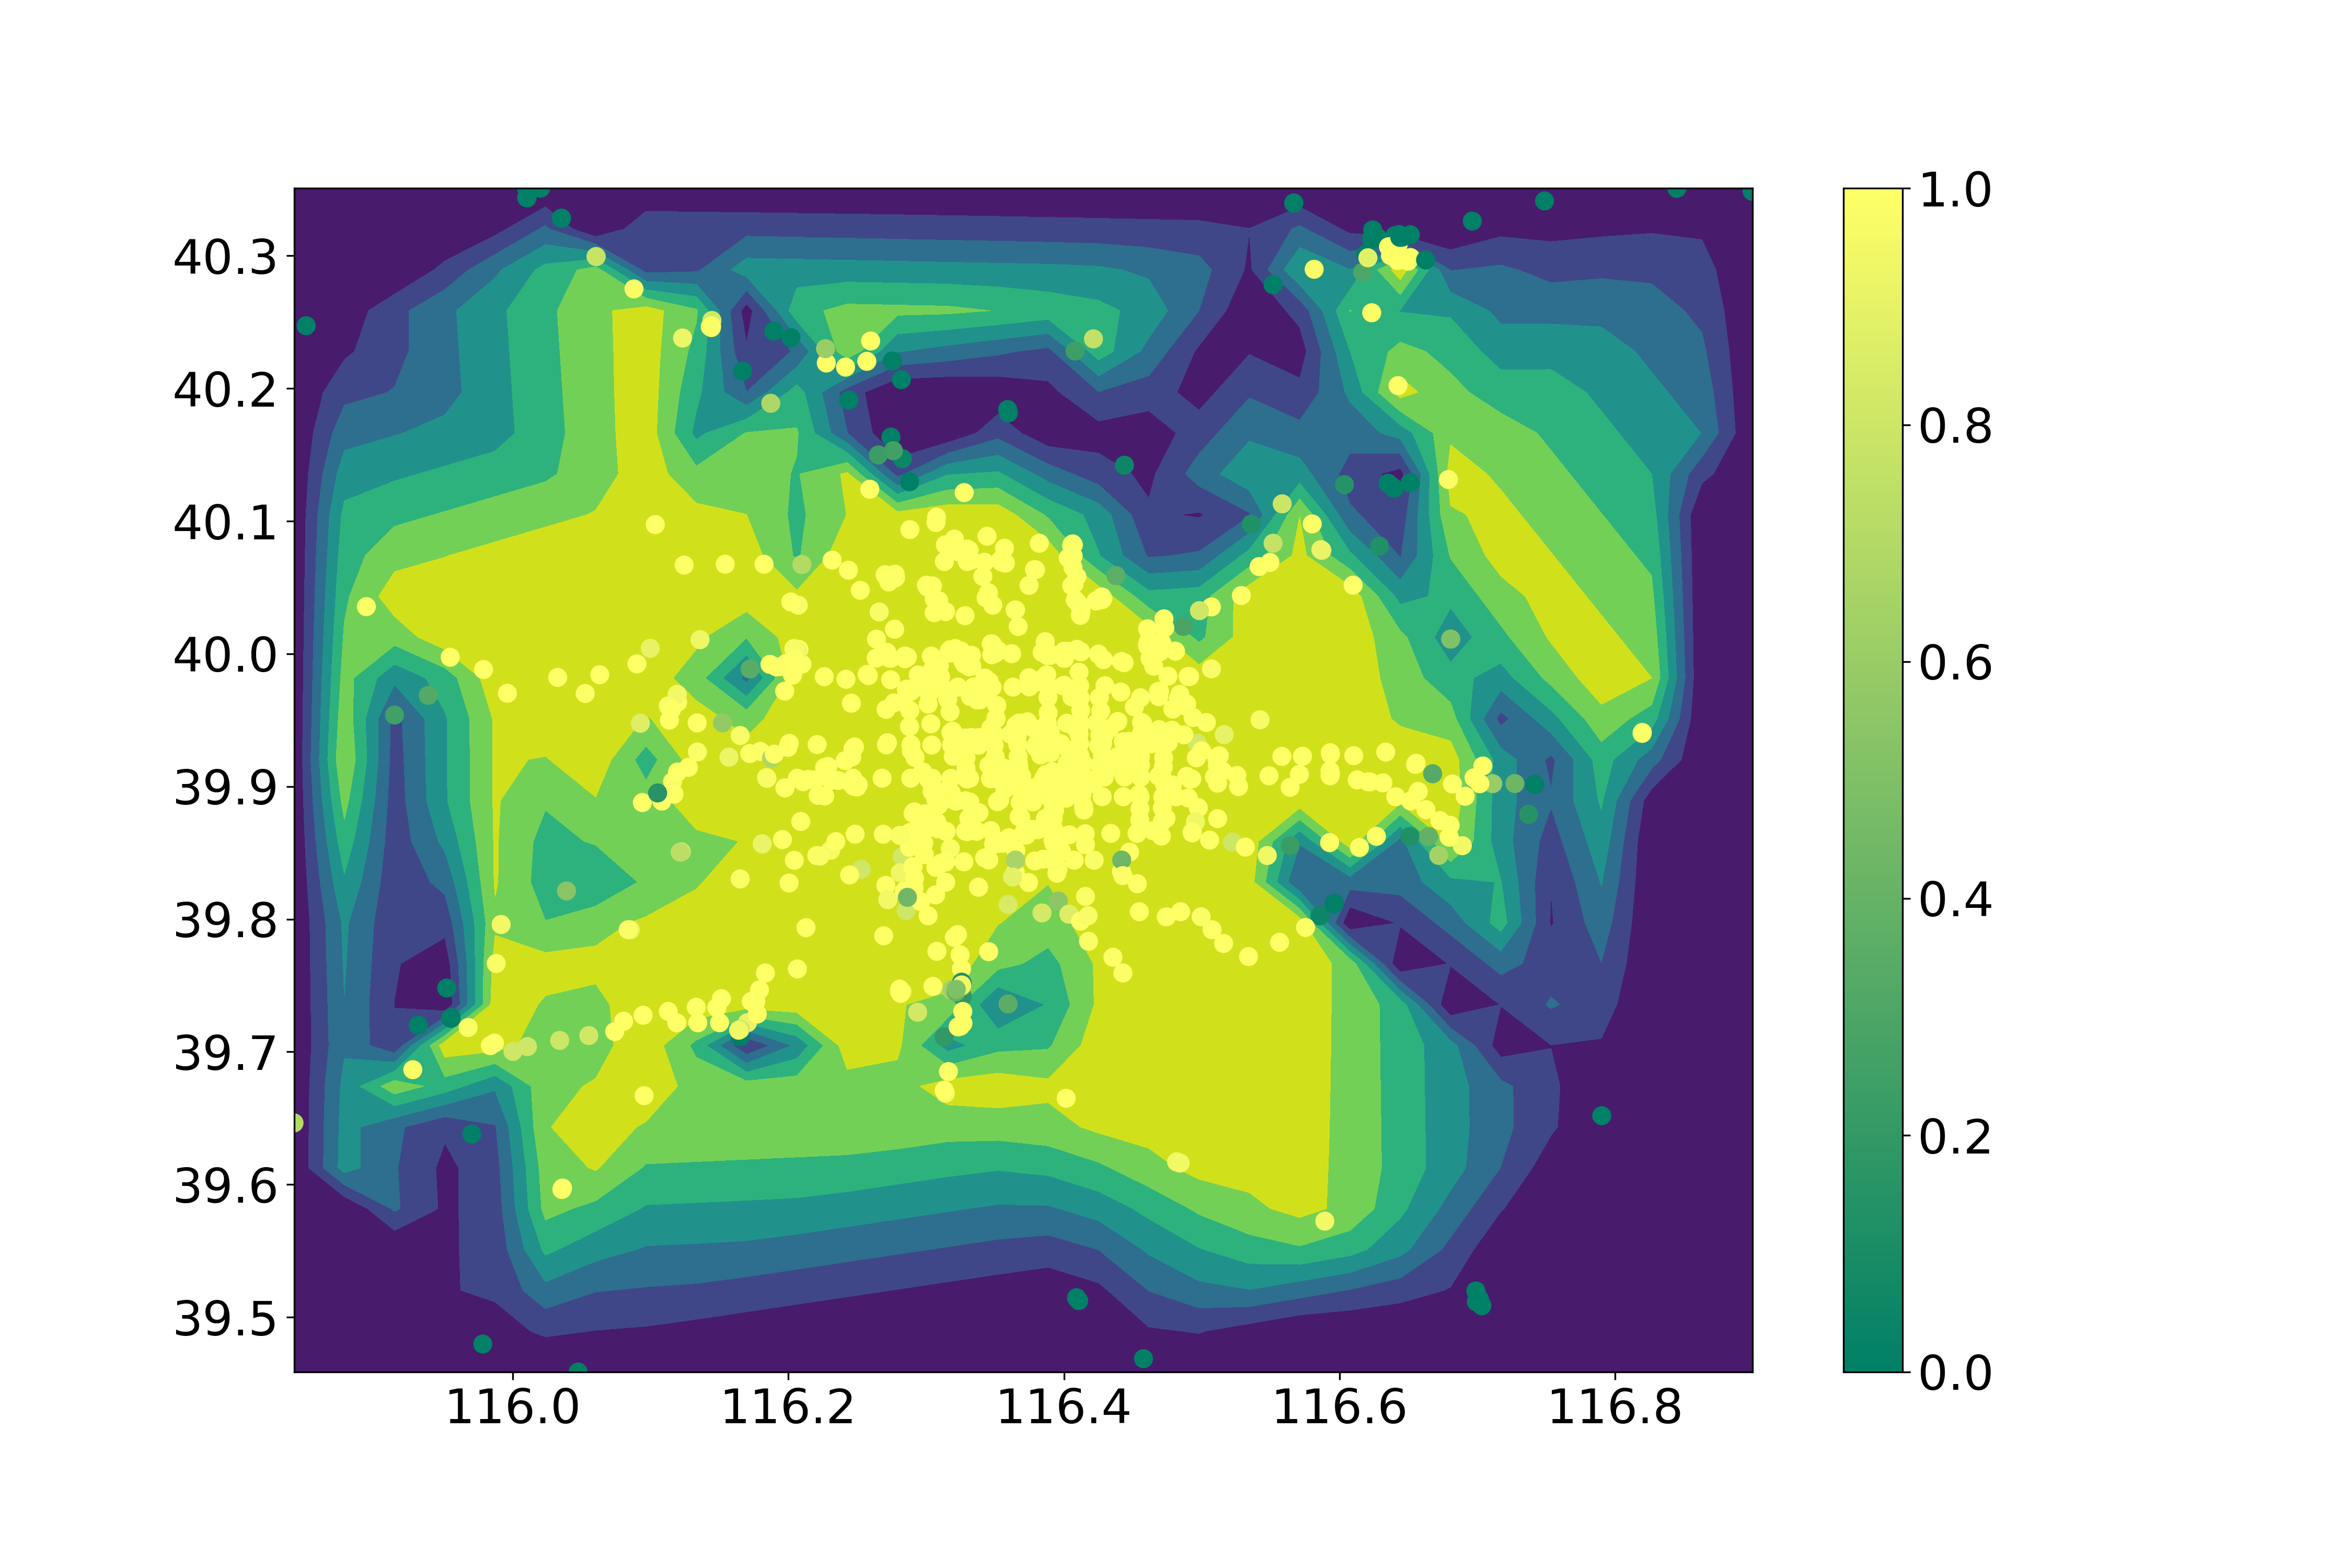
\includegraphics[width=\linewidth]{POIs_coverages_0,00142857_lambda_heatmap.png}
		\caption{Mappa di calore ottenuta per $\lambda = 1/700$}
	\end{subfigure}
	\caption[Risultati POIs, $\lambda = 1/700$]{I risultati ottenuti applicando il modello ai punti di interesse con $\lambda = 1/700$}
	\label{fig:POIs_coverage3}
\end{figure}

\section{Analisi dei risultati ottenuti}

Procediamo adesso con una analisi dei risultati ottenuti per ciascuno scenario e, più in generale, per tutta la sperimentazione.

Le meshgrid e le mappe di calore mostrano la Data Coverage in relazione alle diverse locazioni di raccolta dati. 
La differente scelta delle locazioni ha chiaramente influenzato la mappa di Data Coverage risultante; questo è particolarmente evidente nel caso degli scenari sui flussi di traffico e sui punti di interesse, in cui la relativa sparsità delle locazioni, e la loro assenza nelle zone periferiche della città, porta a dei risultati peculiari.
Ciononostante è bene ricordare che, per i fini specifici del monitoraggio dei flussi di traffico e dei punti di interesse, non siamo interessati a zone con assenza di traffico umano, di conseguenza il risultato ci sembra soddisfacente, ed in linea con le aspettative per ciascuno scenario.
Nelle mappe di calore riguardanti lo scenario di monitoraggio ambientale, si riescono a distinguere bene zone periferiche affatto trafficate, poiché la natura delle locazioni, posizionate a griglia equispaziata, ci permette di valutare con efficacia la Data Coverage in tutta la zona di sensing. Il centro di Pechino ha una Data Coverage praticamente certa e ben distribuita, come si nota dalle figure. 

Fatte queste considerazioni, risulta normale che, ove le locazioni diventino più sparse e distanti dalle traiettorie, la Data Coverage decresca molto rapidamente fino ad arrivare a valori nulli, nelle zone in cui non sono presenti locazioni.
Nei grafici sono evidenti zone con picchi negativi di Data Coverage racchiusi all'interno di aree con una Data Coverage pressoché perfetta.
Questi picchi negativi sono dovuti alla mancanza di traiettorie in quelle specifiche zone, e ci suggeriscono la possibilità di ampliare la strategia di raccolta con piani ad hoc per le suddette zone.

In tutti e tre gli scenari si nota una differenza minima al variare di $\lambda$. Questo è dovuto probabilmente al fatto che le traiettorie, pur aumentate, risultano essere insufficienti a modellare con precisione i pattern di spostamento di persone reali. Per aggiungere realismo alle traiettorie si potrebbero introdurre dei punti di fermata intermedi tra il punto di partenza e quello di arrivo di ciascuna traiettoria sintetica.

Infine, ci sembra opportuno soffermarci brevemente sui limiti del modello.
Poiché $\lambda$ deve modellare il valore di collaboratività degli utenti, è evidente che tale parametro debba essere necessariamente una semplificazione della realtà: con i dati forniti da GeoLife \cite{zheng1, zheng2, zheng3} non possiamo sapere veramente se un utente sarebbe disposto o meno ad accettare una deviazione.
Un altro limite degno di nota è l'aver usato una distribuzione esponenziale nel modello di coverage. Nulla vieta che la probabilità di Data Coverage segua un andamento di tipo diverso, per questo sarebbe interessante provare il modello con altri tipi di distribuzione.
Un'ultima considerazione riguarda le barriere architettoniche e fisiche: nel modello utilizziamo la distanza da una locazione per calcolare la probabilità che un utente sia disposto a raggiungerla e raccogliere i dati, ma  glissiamo sull'esistenza di eventuali barriere architettoniche e fisiche che potrebbero impedire all'utente di raggiungere agilmente la locazione.
Si pensi ad esempio ad una locazione che si trova sulla riva sinistra di un fiume senza ponti: il modello restituirebbe una probabilità di copertura per l'utente che si trova sulla riva destra, tuttavia la raccolta dati sarebbe impossibile, poiché l'utente non avrebbe modo di attraversare il fiume. La Figura \ref{fig:no_coverage_example} mostra questo tipo di problematica.

\begin{figure}
	\centering 
	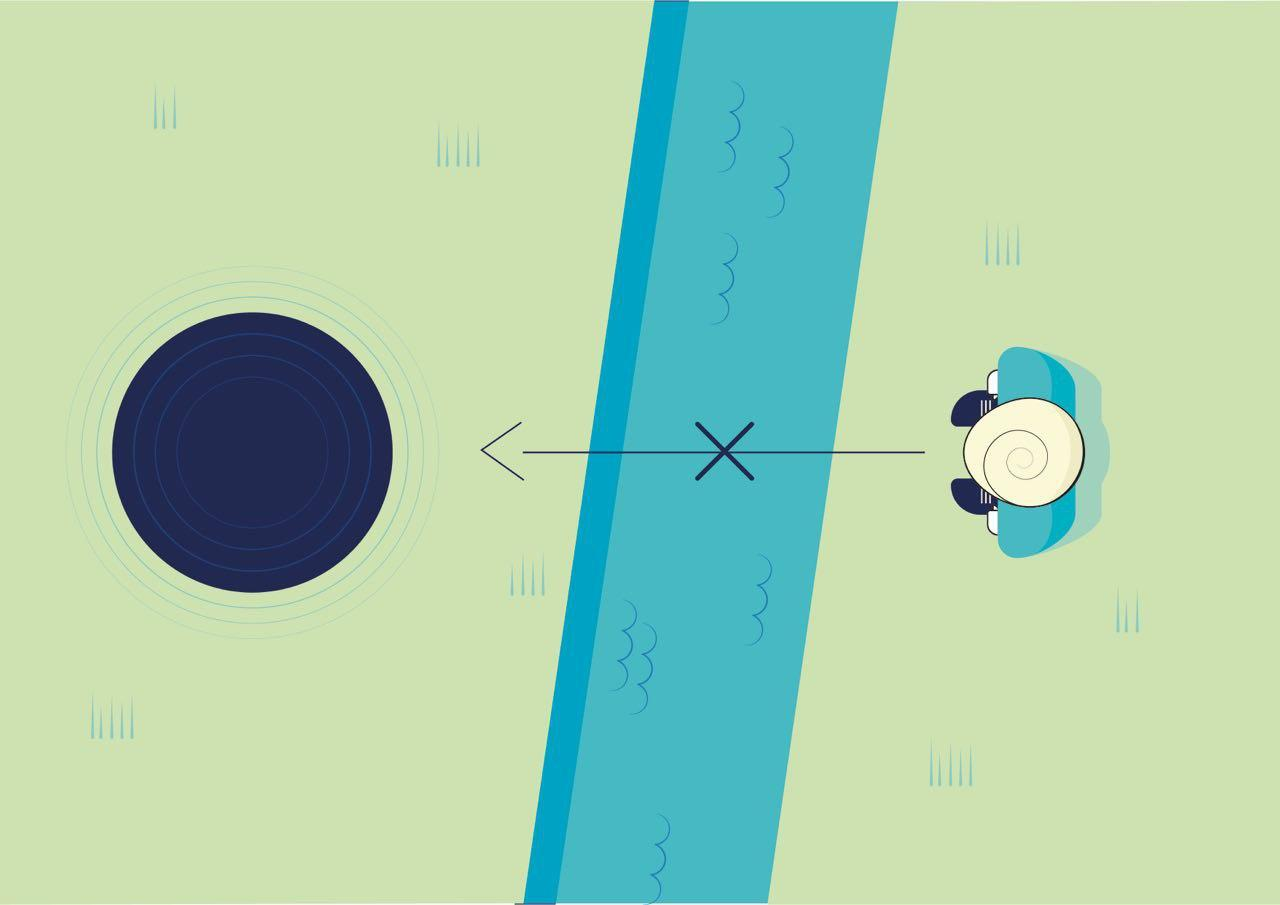
\includegraphics[width=0.7\linewidth]{no_coverage_example.jpg}
	\caption[Esempio di barriera fisica]{Una barriera fisica, in questo caso un corso d'acqua, impedisce all'utente di raggiungere la zona di sensing.}
	\label{fig:no_coverage_example}
\end{figure}

Pur con tutte le semplificazioni citate, i risultati dell'applicazione del modello ci sembrano soddisfacenti, soprattutto in vista di ulteriori sviluppi nella tecnologia del MCS e del miglioramento dei dataset disponibili.